\documentclass[
  fontsize=12pt,
  titlepage=firstiscover,
  paper=letter,
  %twoside,
  oneside,
  cleardoublepage=plain,
  parskip=half-,
  DIV=10,
  parindent,
  appendixprefix,
  chapterprefix,
  listof=totoc,
  %final
]{scrbook}

\usepackage[utf8]{inputenc}

\usepackage[acronym, toc, numberedsection=nolabel, section=chapter]{glossaries}
\setacronymstyle{short-long}
\makeglossaries
\newacronym{os}{OS}{Operating System}
\newacronym{bpf}{BPF}{Berkeley Packet Filter}
\newacronym{ebpf}{eBPF}{Extended \glsentryshort{bpf}}
\newacronym{cbpf}{cBPF}{Classic \glsentryshort{bpf}}
\newacronym{btf}{BTF}{\glsentryshort{bpf} Type Format}
\newacronym{jit}{JIT}{Just-In-Time}
\newacronym{core}{CO-RE}{Compile Once Run Everywhere}
\newacronym{dac}{DAC}{Discretionary Access Control}
\newacronym{acl}{ACL}{Access Control List}
\newacronym{mac}{MAC}{Mandatory Access Control}
\newacronym{mls}{MLS}{Multi-Level Security}
\newacronym{lsm}{LSM}{Linux Security Modules}
\newacronym{krsi}{KRSI}{Kernel Runtime Security Instrumentation}
\newacronym{usdt}{USDT}{User Statically Defined Tracepoints}
\newacronym{pid}{PID}{Process ID}
\newacronym{tid}{TID}{Thread ID}
\newacronym{tgid}{TGID}{Task Group ID}
\newacronym{uts}{UTS}{Unix Timesharing System}
\newacronym{uid}{UID}{User ID}
\newacronym{gid}{GID}{Group ID}
\newacronym{euid}{EUID}{Effective \glsentrylong{uid}}
\newacronym{egid}{EGID}{Effective \glsentrylong{gid}}
\newacronym{tcb}{TCB}{Trusted Computing Base}
\newacronym{cots}{COTS}{Commercial Off-The-Shelf}
\newacronym{ipc}{IPC}{Inter-Process Communication}
\newacronym{ip}{IP}{Internet Protocol}
\newacronym{toctou}{TOCTOU}{Time of Check to Time of Use}
\newacronym{isa}{ISA}{Instruction Set Architecture}
\newacronym{fpga}{FPGA}{Field-Programmable Gate Array}
\newacronym{abi}{ABI}{Application Binary Interface}
\newacronym{api}{API}{Application Programming Interface}
\newacronym{aslr}{ASLR}{Address Space Layout Randomization}
\newacronym{kaslr}{KASLR}{Kernel \glsentryshort{aslr}}
\newacronym{mmu}{MMU}{Memory Management Unit}
\newacronym{tlb}{TLB}{Translation Lookaside Buffer}
\newacronym{vm}{VM}{Virtual Machine}
\newacronym{lxc}{LXC}{Linux Containers}
\newacronym{cpu}{CPU}{Central Processing Unit}

\usepackage{findlay}
\usepackage{langs}
\usepackage{epigraph}

% for changing margins in titlepage
\RequirePackage{geometry}

% for 1.5 line spacing
\RequirePackage{setspace}
\doublespacing%
% single spacing for table of contents
\AfterTOCHead{\singlespacing}

% recompute page layout based on the above
\recalctypearea%

% Use rmfamily for chapters, sections, etc.
\addtokomafont{disposition}{\rmfamily}

% Fix top and bottom margins
%\newgeometry{margin=1in}

% Uncomment this to help debug layout
%\usepackage{showframe}

\setcapindent{0pt}

\newcommand{\bpfbox}{\textsc{BPFBox}}
\newcommand{\bpfcontain}{\textsc{BPFContain}}

\addbibresource{refs.bib}

\title{A Practical, Light-Weight, and Flexible Confinement Framework in eBPF}
\author{William P.~Findlay}
\date{August, 2021}

\hyphenation{App-Armor}

% Remove spurious dot in figure/table captions
\renewcommand*{\figureformat}{%
  \figurename~\thefigure%
}
\renewcommand*{\tableformat}{%
  \tablename~\thetable%
}

\begin{document}

% ==============================================================================
% Cover Page, Abstract and TOC
% ==============================================================================

% Title page
\makeatletter
\begin{titlepage}
    \newgeometry{margin=0.8in}
    \begin{center}
      \vspace*{1cm}
      {\LARGE\bfseries \@title}

      \vspace{1cm}
      by
      \vspace{1cm}

      {\itshape\large \@author\/}

      \vfill

      A thesis submitted to the Faculty of Graduate and Postdoctoral Affairs\\
      in partial fulfillment of the requirements for the degree of

      \vspace{3cm}
      {\bfseries Master of Computer Science}
      \vspace{3cm}


      {\@date}
      \vspace{0.5cm}

      Carleton University\\
      Ottawa, Ontario
      \vspace{0.5cm}

      \copyright{}~2021 \@author%
    \end{center}
\end{titlepage}
\makeatother


\frontmatter%

\chapter*{Abstract}%
\addcontentsline{toc}{chapter}{Abstract}%
\todo{ABSTRACT HERE}
\cleardoublepage%

\chapter*{Acknowledgements}%
\addcontentsline{toc}{chapter}{Acknowledgements}%
\todo{ACKNOWLEDGEMENTS HERE}
\cleardoublepage%

\chapter*{Prior Publication}%
\addcontentsline{toc}{chapter}{Prior Publication}%
\todo{PRIOR PUBLICATION HERE}
\cleardoublepage%

% TOC
\begingroup
\hypersetup{linkcolor=black}
\tableofcontents
\begingroup
\listoffigures
\listoftables
\endgroup

\mainmatter%

% ==============================================================================
% Main Chapter Content Here
% ==============================================================================

\chapter{Introduction}%
\label{c:introduction}
Virtualization is not confinement. To security experts, this may be an obvious statement,
but these two concepts are often conflated, leading to dangerous assumptions about
security in practice. To see why virtualization and confinement are disparate concepts,
consider the goals of each. \textit{Virtualization} describes the goal of providing
a unique, private mapping of shared system resources to a particular subject~\todo{CITE}
(be it a process, a virtualized operating system, or something else).
\textit{Confinement}, on the other hand, describes the goal of restricting a subject's
access to system resources or other subjects~\todo{CITE}. In other words, virtualization
is about \textit{what we can see}, whereas confinement is about \textit{what we can do}.
It should now be abundantly clear not only that virtualization and confinement are two
entirely different concepts, but that virtualization must be combined with confinement to
offer any practical security guarantees.

Container technologies on Linux offer a motivating example of the difference between
virtualization and confinement and how conflating the two can result in problematic
misunderstandings about the security of a system. From first principles, a container is
nothing more than a group of associated processes (and system resources) managed by some
container management engine (e.g.~Docker or \textit{lxc}). While often used for dependency
management, containers also offer lightweight virtualization and confinement using
a series primitives exposed by the operating system kernel. Namespaces and cgroups
virtualize system resources while confinement layers such as \texttt{seccomp(2)} provide
some degree of isolation from the rest of the system~\todo{CITE}. Unfortunately, while
virtualization primitives are widely used in container deployments, the use of confinement
primitives is often overlooked, oversimplified, or overly permissive (i.e.~misconfigured)
in practice~\todo{CITE}.

Despite their name, containers do a very poor job of actually \textit{containing}
a running process.  The Linux kernel already supports a set of strong virtualization
primitives, namespaces and cgroups, that can be used to provide a process with a fairly
compartmentalized view of its environment. But these virtualization primitives do little
to improve the \textit{security} of the applications that use them. Rather, such
virtualization serves much the same purpose as virtualization in other areas of computer
science\,---\,to allow two pieces of code to use the same name for different things and to
abstract away the complex details of the underlying system.

This thesis argues that the key to truly isolating containers from the rest of the system
lies in improving our confinement frameworks to work well in containerized applications.
The status quo of process confinement on Linux is a motley collection of unrelated
technologies, each designed for a specific purpose, often beyond the scope of simple
process confinement. Container management solutions cobble these technologies together,
applying over-permissive, coarse-grained defaults or compiling simple policies into
a complex entanglement. To rectify the status quo, we must rethink confinement from the
ground up, and build a confinement framework designed to be aware of the container model
of computation.

In particular, we posit that the root of the confinement problem in container security
lies in a semantic gap between the containers themselves and the confinement primitives
that are used to secure them. Many academics have recognized this semantic gap. Some have
attempted to rectify it by introducing mechanisms for automatic policy derivation based on
container images (e.g.~the Docker image manifest) or observed behaviours at
runtime~\todo{CITE ALL EXAMPLES}. Others have attempted to introduce new layers of
abstraction to security policies~\todo{CITE Snap et al} or into the kernel
itself~\todo{CITE security namespaces}. \todo{WHY ARE THESE BAD IN ONE SENTENCE?} We
propose that the heart of the problem lies in the fact that the Linux kernel itself has no
single representation of \textit{what exactly a container is} from a security standpoint.

One approach would be to extend the container with a container-aware LSM, but maintaining
out-of-tree kernel modules is challenging, as such a module would need to be continually
updated as the kernel evolves. Further, end-users may be reluctant to adopt and
out-of-tree solution, particularly in production environments with low risk-tolerance.
Even worse, a static security mechanism is unlikely to work well for all use
cases\,---\,some users (e.g.~operators of multi-tenant container clouds) would like to
totally isolate containers from each other, while use cases (e.g.~microservices
deployments) may require individual containers to communicate and cooperate with each
other. Thus, our solution should be practical, light-weight, and flexible such that we can
define a container-level policy enforcement mechanism that can be readily adopted in
production use cases. A relatively new Linux technology, \textit{Extended Berkeley Packet
Filter} (eBPF), offers the opportunity to design such a system.

To improve the status quo of confinement on Linux, we present two research prototypes,
\bpfbox{} and its successor, \bpfcontain{}. The former is a novel application sandboxing
framework, and the latter extends that framework to work well in the context of container
security. Both research systems are implemented using eBPF, a new Linux kernel mechanism
for dynamically attaching simple filter programs to various system events and aggregating
data from these events in kernelspace~\cite{gregg2019_bpf, starovoitov2014_ebpf}.
Specifically, we use the new LSM program type~\cite{singh2019_krsi}, introduced in Linux
5.7, to attach eBPF programs to Linux Security Module hooks. Using eBPF, we can safely
extend the kernel at runtime, building a new confinement model that suits the container
use case without detracting from existing confinement implementations or tying the kernel
down to one particular model.


\section{Motivation}%
\label{s:motivation}

\subsection{Contextualizing the Problem}%
\label{ss:contextualizing-the-problem}

Containers are \textit{everywhere}. In the cloud, containers form the backbone of
cloud-native computation. Kubernetes~\todo{CITE} clusters drive the microservices that
power scalable web applications. In devops, Docker~\todo{CITE} containers often form the
backbone of continuous integration workflows, providing reproducible environments for
development, testing, and debugging. On the desktop, containerized package managers like
Snap~\todo{CITE}, FlatPak~\todo{CITE}, and AppImage~\todo{CITE} offer self-contained,
isolated software bundles, facilitating a smooth software installation process (mostly)
free of dependency management concerns.

Despite a steadily increasing prevalence, containers face major adoptability challenges in
deployments where they are expected to outright replace virtual machines. Unlike virtual
machines, which are abstracted away from the host and interact with a hypervisor,
containers interact directly with the host operating system kernel. This means that, while
much lighter-weight than hypervisor-based virtualization, containers are inherently less
isolated from each other and from the host system in
general~\cite{sultan2019_container_security, xin2018_container_security,
mullinix2020_security_measures, bui2015_docker_analysis}.  In order to have truly secure
containers, we must take great care to ensure that a container is properly
\textit{confined}. In practice, this means restricting the processes that run within the
container from performing certain actions that can negatively impact or damage the system.
As we have already discussed, virtualization primitives alone are not enough to achieve
proper isolation. These primitives \textit{must} be combined with confinement mechanisms
and these confinement mechanisms \textit{must} be applied properly. Otherwise, we risk
overprivilege, resulting in potential violations of our security model.

Container security issues are widely studied in the
literature~\cite{sultan2019_container_security, xin2018_container_security,
mp2016_hardening, mullinix2020_security_measures, bui2015_docker_analysis}.  Given that
containers offer weaker isolation guarantees than alternatives like hardware virtual
machines (HVMs)~\todo{CITE} or even paravirtualization~\todo{CITE}, one might be inclined
to assume that container security would be of paramount importance. Contrary to this
assumption, container management frameworks take a lax attitude towards the enforcement of
least-privilege, provisioning overly-permissive blanket default policies and relying on
a complex suite of ill-suited security mechanisms provided by the host system.

Docker, for instance, applies a default AppArmor policy revoking access to only the most
sensitive kernel interfaces like procfs and sysfs and disabling the ability to mount new
filesystem.  Beyond these basic controls, the container has full permission to access all
filesystem and resources, has access to several POSIX capabilities, and may unmount any
filesystem~\cite{docker_apparmor, docker_default_apparmor}. Even worse, a kernel that does
not support AppArmor or that is not properly configured is left totally bereft of this
protection to begin with.  Docker complements its default AppArmor profile with a set of
sensible seccomp rules, revoking access to many privileged system calls. While such
a policy \textit{does} help to harden the container, it remains
overly-generalized~\cite{sultan2019_container_security} and does not uniquely capture the
needs of every container deployment. Users who wish to grant additional permissions to
their container are left with the choice of either writing and auditing custom AppArmor
and seccomp policies or outright disabling protections altogether with the
\texttt{--privileged} flag.

Docker is but the most prominent example among many. In general, all existing container
management frameworks rely on a patchwork of isolation mechanisms, each enforcing its own
confinement policy and each with varying degrees of generalization. As a result, these
policies are often difficult to reason about, and thus difficult to effectively audit.
A vulnerability in any individual mechanism or a misconfiguration in any individual policy
opens the container or the host system itself up to attack. Blanket defaults are often
ineffective for specific use cases and result in situations where the end-user is forced to
either abandon all hope of security or muddle through the configuration of multiple policy
enforcement mechanisms.

\subsection{Why Design a New Confinement Framework?}%
\label{ss:why-new}

The process confinement problem dates back half a century~\cite{lampson1973_confinement}.
Since the advent of multi-processing \todo{IN WHAT YEAR? (e.g.~with Unix in 196X) CITE},
security experts have been concerned with designing systems in such a way that two running
programs minimally interfere with one another. Since then, an abundance of tools and
frameworks, some more practical than others, have been proposed to limit the damage that
untrusted software can do to the system as a whole~\cite{shu2016_security_isolation_study}.
These are covered in more depth in \Cref{c:background}. For now, we focus on why it might be
prudent to design yet another confinement framework amidst this veritable ocean of prior work.

The Linux kernel already provides a number of confinement primitives. Seccomp allows for
a process to confine itself by filtering the system calls it can make. Mandatory access
control solutions based on LSM (Linux Security Modules) hooks can be configured to define
and enforce powerful per-application policies, protecting system resources from unwanted
access. Unix DAC (discretionary access control) restricts access to system resources
according to resource owners, groups, permission bits, and access control lists. When
applied to container security, the common problem faced by these security mechanisms is
that they are being applied to solve a problem for which they were not originally
designed. To solve this problem, we seek to design a unifying security abstraction for
containers and apply this abstraction to enforce per-container policy in kernelspace.

From the kernel's perspective, a containerized process is just like any other. While it
may be virtualized under one or more namespace and process control groups, there is no
precise definition of what exactly constitutes a \textit{container}. This lack of a solid
abstraction widens the semantic gap between traditional policy enforcement mechanisms and
security policy designed to protect containers. In defining a new policy enforcement
mechanism focused specifically on containers, we have an opportunity to narrow this
semantic gap, simplify the resulting policies, and eliminate the need to combine several
security mechanisms together to do a job that could be accomplished by just one. Since our
proposed solution is based on eBPF, it requires no modification of the kernel and can be
dynamically loaded at runtime.  This means that we can provide such a unified abstraction
without sacrificing forward or backward compatibility with alternative approaches.

\subsection{Why eBPF?}%
\label{ss:why-ebpf}

An eBPF-based confinement mechanism provides several advantages over traditional
confinement models.  Firstly, eBPF is \textit{light-weight}. eBPF programs can monitor
many aspects of system behaviour, from userspace function calls to kernelspace function
calls, system calls, security hooks, and the networking stack. Data from these events can
be aggregated in real time in kernelspace, providing an extensible, performant, and
flexible framework for modelling relationships and enforcing policy decisions based on
these relationships.  A single security mechanism based on eBPF can combine the advantages
of several disparate mechanisms that would ordinarily need to be combined together to
provide full protection. This property precisely mirrors the way container security is
currently done on Linux. Rather than combining namespaces, cgroups, seccomp, and mandatory
access control together, eBPF provides the opportunity to design a single framework
providing the advantages of each.

A second advantage of eBPF for writing a security framework is that it is
\textit{dynamic}. eBPF programs can be loaded into the kernel dynamically and attached to
multiple events. Instrumenting a system event with eBPF can be done at runtime,
\textit{without} the need to modify the kernel in any way.  Similarly, eBPF maps, the
canonical runtime data store for eBPF programs, can be loaded, unloaded, modified, and
queried at runtime from both userspace and kernelspace, providing a rich substrate for
a dynamic model of system behaviour. These properties culminate in the ability to design
a flexible security mechanism without tying the kernel down to any one particular
abstraction. In the context of container security, this is a particularly important goal,
as containers are traditionally a \textit{userspace} concept, glued together with various
abstractions provided by the kernel.

\textit{Production-safety} is a third advantage provided by eBPF. All eBPF programs go
through a verification process before they are loaded into the kernel. The eBPF verifier
analyzes the program, asserting that it conforms to a number of safety requirements, such
as program termination\footnote{This property is enforceable due to the fact that eBPF
programs are not Turing complete~\cite{gregg2019_bpf}.}, memory safety, and read-only
access to kernel data structures. While itself not formally verified, the eBPF verifier
facilitates the adoption of new eBPF programs into production use cases, since an eBPF
program is far less likely to adversely impact a production system than other methods of
extending the kernel (e.g.~kernel patches and loadable kernel modules). In fact, eBPF is
already being used in production at large datacenters by Facebook, Netflix, Google, and
others to monitor server workloads for security and performance
regressions~\cite{gregg2019_bpf}. These factors make eBPF a promising choice for
designing an \textit{adoptable} security mechanism.

In summary, eBPF offers unique and promising advantages for developing novel security
mechanisms. Its light-weight execution model coupled with the flexibility to monitor and
aggregate events across userspace and kernelspace provide the ability to control and audit
nearly any aspect of the running system. eBPF maps, shareable across programs and between
userspace and the kernel offer a means of aggregating data from multiple sources at
runtime and using it to inform policy decisions across domains. A security mechanism based
on eBPF can be dynamically loaded into the kernel as needed, and eBPF's safety guarantees
combined with its increasing adoption in production use cases provide strong adoptability
advantages. This means that a security mechanism based on eBPF can be both adoptable and
effective.


\section{Contributions}%
\label{s:contributions}

This thesis offers three principle contributions to the field of computer science.
They are summarized as follows:
\begin{itemize}
  \item \todo{Enumerate contributions}
  \item \todo{Enumerate contributions}
  \item \todo{Enumerate contributions}
\end{itemize}

\section{Outline}%
\label{s:outline}

The rest of this thesis proceeds as follows. \Cref{c:background} presents background on
virtualization and process confinement, historical confinement techniques that have been
employed in Linux and other Unix-like operating systems, and eBPF and its applications to
performance and security monitoring. \Cref{c:bpfbox} describes the design and
implementation of \bpfbox, presents an initial performance evaluation, and~\todo{What
else?  Need to figure out how much I want to say about \bpfbox}. \Cref{c:bpfcontain}
presents \bpfcontain, an iteration on the original \bpfbox{} system designed
specifically for container security. We present its design and implementation, evaluate
its performance and effectiveness as a security mechanism in greater detail, and describe
how it can be applied to secure practical container deployments. \Cref{c:discussion}
presents a discussion on \bpfbox{} and \bpfcontain{} and discusses opportunities for
future work both in the context of container security and other potential security
applications of eBPF beyond the scope of confinement. \Cref{c:related} surveys existing
literature in the confinement space and compares \bpfbox{} and \bpfcontain{} to extant
approaches. \Cref{c:conclusion} concludes.


\chapter{Background and Related Work}%
\label{c:background}
This chapter presents technical background information required to understand this thesis
and discusses related work from the perspective of industry and academia.
\Cref{s:process-security-model} presents technical background on historical models for
process-level confinement, with a particular emphasis on Multics, Unix, and Unix
derivatives.  \Cref{s:security-extensions} focuses on subsequent extensions to the Unix
security model and covers related work in the confinement space. \Cref{s:virtualization}
examines process-level virtualization technologies in Unix-like operating systems.
\Cref{s:containers-bg} discusses the differences between hypervisor- and container-based
virtualization, container security, and presents related work in the container security
space. Finally, \Cref{s:ebpf-bg} presents a detailed history of \glsentryshort{ebpf},
describes its architectural components and features, and discusses use cases in security
and beyond.

\section{Classic Unix Process Security Model}%
\label{s:process-security-model}

This section reviews foundational concepts in \gls{os} (particularly Unix-like \gls{os}s
and Linux) security. In particular, we discuss the \textit{reference monitor concept},
\textit{virtual memory and user processes}, and \textit{discretionary access control} and
how these concepts interact to form the backbone of process-level security in Unix.  The
goal of this section is to help the reader build a mental model of how operating systems
isolate and protect processes and system resources at the most fundamental level. Readers
familiar with these \gls{os} security concepts can skip this section in favour of
\Cref{s:security-extensions} which examines more advanced security mechanisms and
discusses related work.

\subsection{The Reference Monitor}%
\label{ss:refmon}

The \textit{reference monitor concept}, first introduced in the landmark 1972 Anderson
Report~\cite{anderson1972_report}, was among the earliest complete descriptions of a full
access control mechanism and remains influential in operating system design to date. The
reference monitor is an abstract model for a secure reference validation mechanism built
into the operating system. The model partitions the system into \textit{subjects} (users,
processes, etc.) and \textit{objects} (system resources).  Subjects request access to
objects and the reference monitor checks this access against a known list of allowed
accesses, parameterized by the subject, object, and requested access. The software
implementation of a reference monitor is known as the \textit{security kernel.}
\Cref{fig:refmon} depicts the reference monitor concept as it was first presented by
Anderson~\cite{anderson1972_report}.

\begin{figure}[htbp]
  \centering
  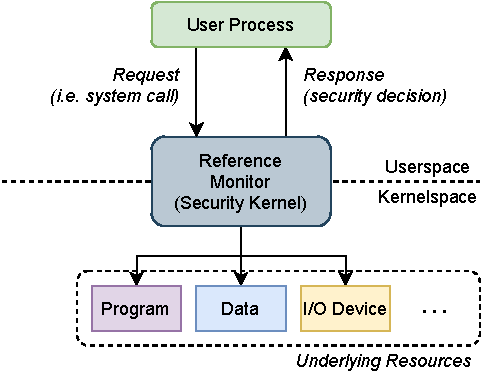
\includegraphics[width=0.6\linewidth]{figs/background/refmon.pdf}
  \caption[The reference monitor concept]{
    The reference monitor concept as outlined in the Anderson Report. Redrawn and adapted
    from Anderson~\cite{anderson1972_report}. User processes make requests (e.g.~via
    system calls to the operating system). The \gls{os} kernel invokes the reference
    monitor, which is implemented in software as a security kernel. The reference monitor
    queries its security policy taking the subject, object, and other parameters as input.
    As output, it returns a security decision (i.e.~whether the requested access should be
    \textit{allowed} or \textit{denied}).
  }%
  \label{fig:refmon}
\end{figure}

While the majority of modern operating systems do not include a security kernel as
described by Anderson, the reference monitor architecture has informed the design of
modern access control mechanisms and models the reference validation process that occurs
when the kernel is servicing userspace requests (i.e.~system
calls)~\cite{van_oorschot2020_tools_jewels}. In order for such a design to be considered
valid, Anderson enumerates three key properties: (i) Tamper Resistance; (ii) Complete
Mediation; and (iii) Verifiability. These properties facilitate reasoning about the
security of modern access control mechanisms, even if they do not strictly adhere to the
reference monitor model.

\paragraph*{Tamper-Resistance}

In order for the reference monitor to be considered \textit{tamper-resistant}, an unauthorized
party must not be able to alter the reference monitor's code or modify any data
(e.g.~memory, persistent storage) that the reference monitor relies on to enforce correct
reference validation~\cite{anderson1972_report}. This property follows from the fact that
unauthorized tampering with the reference monitor totally invalidates any security
guarantees.

\paragraph*{Complete Mediation}

The property of \textit{complete mediation} means that the reference monitor should be
invoked on all security sensitive events. It should be impossible for an attacker to
bypass the reference monitor in any way. Any software that is not subject to reference
validation should be considered a part of the reference
monitor~\cite{anderson1972_report}.

\paragraph*{Verifiability}

\textit{Verifiability} refers to the ability to reason about or prove the correctness of
the reference monitor (i.e. that the first two properties hold). Formal verification methods
are the best way of achieving verifiability, although this may not necessarily be practical
for highly complex systems. For this reason, it is recommended to design the reference monitor
in such a way that verifiability is maximized~\cite{anderson1972_report}.

\subsection{Virtual Memory and Memory Protection}%
\label{ss:virtual-memory}

Virtual memory~\cite{denning1970_virtual} is a mechanism for mapping \textit{virtual}
memory addresses to \textit{physical} machine addresses. First introduced in the 1950s,
the original goal of virtual memory was to make it easier for programmers to manipulate
memory without worrying about the underlying details of storage
configuration~\cite{denning1970_virtual}. With the advent of multi-processing systems,
virtual memory took on a new role\,---\,separation of memory resources between distinct
user processes. This separation is a fundamental notion for secure multi-processing; two
user processes should not be able to interfere with each other's memory, and a user
process should not be able to interfere with the \gls{os} kernel, resident in ring
0 memory.

By partitioning memory into virtual address spaces, virtual memory forms the most
fundamental isolation barrier between user processes. To accomplish this goal, a hardware
mechanism, the \gls{mmu}, translates virtual addresses to physical addresses using
a \textit{page table} maintained by the operating system in main memory. To accelerate the
translation of memory addresses, modern processors cache this mapping in a specialized
cache area called the \gls{tlb}.  In Unix, each user process gets its own virtual address
space by default, maintained in a per-process page table. Where necessary, this isolation
may be voluntarily broken using memory sharing mechanisms provided by the \gls{os} kernel
(e.g.~multi-threading or shared memory mappings). The kernel also gets its own address
space which maps the entirety of physical memory.

While virtual memory can help isolate user processes from each other and user process from
the kernel, additional protection mechanisms are required to strengthen this isolation. To
this end, the CPU \gls{isa} generally defines memory protection bits that can be applied
to physical pages and enforced in the \gls{mmu}. For instance, individual pages can be
marked as readable, writable, and/or executable depending on how the memory is to be used.
How these protections are used is generally up to the operating system; for instance,
modern operating systems often enforce a policy where pages marked writable and not
allowed to be marked executable and vice versa (this is often referred to as W$\oplus$X).
This helps to prevent the most baroque code execution attacks. Another important
protection mechanism employed by the operating system is \gls{aslr}, which slightly
randomizes virtual address space mappings, making them unpredictable and thus harder for
attackers to exploit consistently. A similar mechanism, \gls{kaslr}, protects the kernel.
The \texttt{grsecruity} patch suite~\cite{grsecruity} offers additional memory protection for the
Linux kernel, hardening the boundary between userspace and kernelspace and applying
additional mitigations to prevent return-oriented programming attacks.

Additional protections are afforded by \textit{memory protection rings}, a concept first
introduced by Multics~\cite{vyssotsky1965_multics, corbato1965_multics} in the mid-1960s.
In the original design, 64 protection rings were defined in hardware, numbered from 0--63.
A task running in a higher-numbered protection ring would be unable to access any memory
marked with a lower-numbered protection ring, effectively isolating sensitive code and
data from unprivileged tasks. Modern CPUs carry forward this notion of protection rings,
although a typical modern processor only defines \textit{four} protection rings rather
than 64. Modern \gls{os}s, including Linux, generally only use \textit{two} of these
rings, ring 0 and ring 3 for kernelspace and userspace respectively. \Cref{fig:rings}
depicts this design. Lee \etal~\cite{lee2018_lotr} have proposed using the remaining two
rings for finer-grained isolation on x86.

\begin{figure}[htbp]
  \centering
  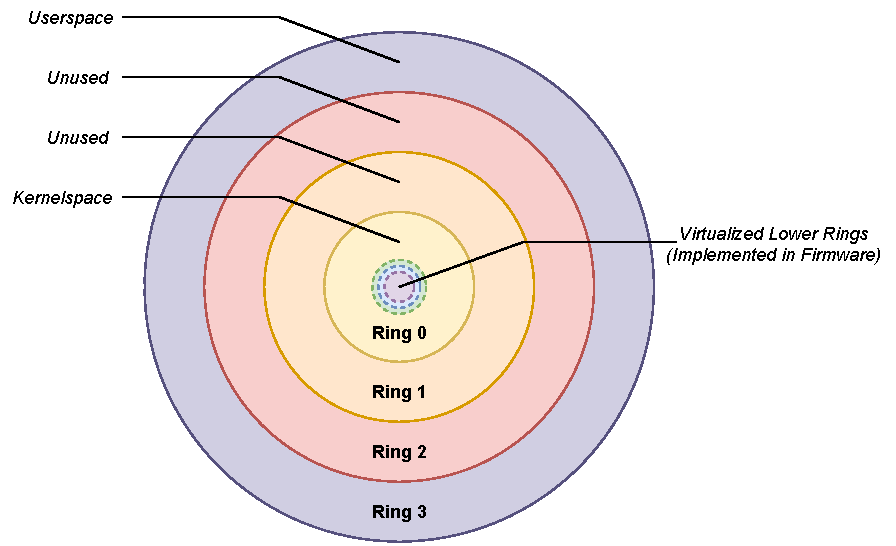
\includegraphics[width=0.8\linewidth]{figs/background/rings.pdf}
  \caption[Protection rings on modern CPUs]{
    A visualization of protection rings on modern CPUs. Ring 3 contains
    \textit{userspace}, the address space of ordinary applications that run in user mode.
    Ring 0 contains \textit{kernselspace}, the kernel's address space. Code running in
    ring 0 is said to run in \textit{supervisor mode}. Rings 1--2 are generally unused by
    \glsentryfull{cots} operating systems.  Modern CPUs often implement \enquote{lower}
    rings (-1, -2, etc.) by virtualizing ring 0 in firmware. These are typically reserved
    for the hypervisor and other hardware-backed features like Intel's System Management
    Mode~\cite{tereshkin2009_introducing}.
  }%
  \label{fig:rings}
\end{figure}

\subsection{Discretionary Access Control}%
\label{ss:dac}

\textit{Discretionary access control} (DAC) comprises the most basic form of access
control in many operating systems, including Linux, other Unix-like operating systems, and
Microsoft Windows. First formalized in the 1983 US Department of Defense
standard~\cite{orange_book}, a discretionary access control mechanism partitions and
labels system objects (i.e.~resources such as files) by the subjects (i.e.~actors such as
users and user processes) that \textit{own} them. The corresponding resource owner then
has full authority to decide which subjects have access to its owned objects. This notion
of ultimate authority over a subject's owned objects constitutes the primary difference
between discretionary access control and mandatory access control, which is covered in
\Cref{ss:mac}.

Classically, Unix-like systems have implemented discretionary access control in the form
of \textit{permission bits} and \textit{access control lists}. Each process on the system
runs under a specific user and group ID, which uniquely identify the user and group of the
process respectively, where each group is a collection of one or more users. Permission
bits and access control lists denote access permissions according to the user ID and group
ID of the process requesting the resource. These permissions can in turn be overridden by
the \textit{superuser} or \textit{root}~\cite{van_oorschot2020_tools_jewels,
jaeger2008_os_security}.

\subsubsection*{Permission Bits}

Permission bits in Unix are special metadata associated with a file that determine
coarse-grained access to the file according to a subject's \gls{uid} and \gls{gid}.
Permission bits are divided into three sections: \textit{User}, \textit{Group}, and
\textit{Other}. The \textit{User} bits apply to subjects whose \gls{uid} matches the
resource owner's \gls{uid}, while the \textit{Group} bits consider the \gls{gid} instead.
In all other cases (i.e.~when neither the \gls{uid} nor the \gls{gid} matches), the
\textit{Other} bits determine the allowed access. To determine which access should be
allowed, permission bits encode a coarse-grained \textit{access vector}, specifying read,
write, and execute access on a file or directory (in the case of a directory, execute
access implies the ability to \texttt{chdir(2)} into that directory).

While convenient, permission bits are generally insufficient to provide legitimate
security guarantees to modern systems~\cite{van_oorschot2020_tools_jewels,
jaeger2008_os_security}. In particular, permission bits encode coarse-grained permissions
and apply these permissions in a coarse-grained, all-or-nothing, manner. For instance,
consider the use case of granting read-only access to another user. Specifying such access
as part of the \textit{Other} bitmask implies granting access to any user on the system.
Specifying access to a particular \textit{Group} is slightly better, but the resource
owner has no direct control over which other users belong to this group, now or in the
future. Thus, we cannot say with certainty that we may specify such access without
violating our security assumptions.

\subsubsection*{Access Control Lists}

\Glspl{acl} offer a slightly more granular alternative to permission bits,
at the expense of increased complexity~\cite{jaeger2008_os_security,
van_oorschot2020_tools_jewels}. Unlike permission bits, which rely on three coarse-grained
subject categories (\textit{User}, \textit{Group}, and \textit{Other}), an access control
list defines a set of subjects and their corresponding permissions for every object. It
may be helpful to think of this as breaking up the \textit{Other} category into distinct
subjects rather than granting or revoking blanket access to all other users on the system.

Capability lists, complementary to access control lists, define a set of objects and
allowed access patterns for every subject. A capability list for a given subject can be
derived by taking the set of all access control lists for every object and vice
versa~\cite{van_oorschot2020_tools_jewels}. Together, the set of all access control lists
(or capability lists) forms an \textit{access matrix}, describing the \gls{dac} policy over
the entire system. \Cref{fig:acl} depicts this relationship.

\begin{figure}[htbp]
  \centering
  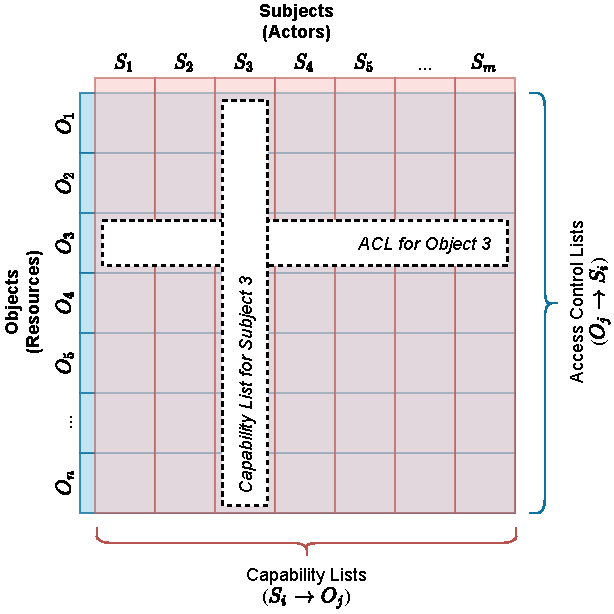
\includegraphics[width=0.8\linewidth]{figs/background/acl.pdf}
  \caption[The access matrix]{
    The access matrix and the relationship between \glspl{acl} and capability
    lists~\cite{anderson1972_report, van_oorschot2020_tools_jewels,
    jaeger2008_os_security}. \glspl{acl} define the set of subjects that have specific
    access rights on a particular object. Capability lists conversely define the access
    rights that a specific subject has on a set of objects. Note that an \gls{acl} may be
    derived by taking the set of all capability lists and vice versa. Taken together,
    these form the access matrix.
  }%
  \label{fig:acl}
\end{figure}

\subsubsection*{The Superuser and Setuid}

To facilitate system administration, many \gls{dac} schemes incorporate the notion of
a \textit{superuser} or \textit{administrator role} into their model. In Unix and
Unix-like operating systems, the superuser or \textit{root} user is denoted by the
\gls{uid} of zero. Any process running with the \gls{euid} of zero is said to be
\textit{root-privileged}. These root-privileged processes can then override the system's
\gls{dac} policy, bypassing permission bits and access control entries on system objects.

In many cases, a program requires additional privileges in order to function. For
instance, a \texttt{login} program would require the ability to read security-sensitive
password entries in \texttt{/etc/shadow}. To achieve such functionality, Unix provides
special \texttt{setuid} and \texttt{setgid} permission bits that implicitly set the
effective user and group IDs of a process to those of the file owner.
A sufficiently-privileged process may also change its own \gls{euid} or \gls{egid} at
runtime using the \texttt{setuid(2)} and \texttt{setgid(2)} family of system calls. The
example login program, for instance, could use these system calls to drop its privileges
to those of the user being logged in. While necessary under the Unix \gls{dac} model,
setuid and setgid binaries have long been the target of exploitation, particularly for
privilege escalation attacks~\cite{dittmer2014_setuid, van_oorschot2020_tools_jewels,
jaeger2008_os_security}.

\subsubsection*{User and Group Assignment}

To alleviate concerns with discretionary access control, systems often take the approach
of assigning a unique user and/or group to a specific application. Such applications are
typically security-sensitive, such as a privileged daemon or network-facing service. This
technique achieves a dual-purpose: firstly, the application can lock down any resources it
owns, simply by restricting any access to its own \gls{uid}; secondly, the resulting
process no longer needs to run under the same \gls{uid} as its parent. This effectively
limits the amount of outside resources that the application can access (so long as
permission bits are correctly configured).

The Android operating system takes this model a step further, assigning a unique \gls{uid}
and \gls{gid} to every application on the system, with optional \gls{uid} sharing between
applications that come from the same vendor. Under this model, no process' \gls{uid} ever
corresponds to a human user. While this arguably improves security, Barrera
\etal~\cite{barrera2012_android} found weaknesses in Android's \gls{uid} sharing model
that can reduce its security to the trustworthiness of an app's signing key.

\subsubsection*{DAC Security Assumptions and Attacks}

Although discretionary access control provides a convenient and intuitive user-centric
model for object ownership and permissions, it makes some dangerous assumptions about
security that can totally invalidate the model in
practice~\cite{shu2016_security_isolation_study}. In particular, DAC assumes that all
processes are benign and contain no exploitable vulnerabilities. The mere existence off
malware and exploitable vulnerabilities (e.g.~memory safety vulnerabilities) immediately
invalidates this assumption. For instance, consider an honest but vulnerable piece of
software running under a given \gls{uid} $X$. An attacker exploiting a vulnerability in
this application could perform arbitrary operations on any files owned by $X$. Similarly,
a Trojan horse\footnote{A Trojan horse is a piece of ostensibly benign software that
is designed to perform some malicious action or actions in addition to its ordinary
functionality~\cite{van_oorschot2020_tools_jewels}.}~\cite{shu2016_security_isolation_study,
van_oorschot2020_tools_jewels} can perform arbitrary malicious operations on $X$'s files
without needing to exploit any vulnerability. The fundamental issue with Unix \gls{dac} is
that these files need not necessarily have \textit{anything} to do with the program in
question.

Another fundamental issue with Unix \gls{dac} lies in the ultimate authority of the root
user. Any process running with \gls{euid}=0 is immediately part of the system's
\gls{tcb}\footnote{The \textit{trusted computing base} is the set of all hardware
and software that must be trusted in order for the system to be considered trusted.
Typically, this includes system hardware, the operating system itself, and a small subset
of userspace programs~\cite{jaeger2008_os_security}.}. The same applies to any executable
marked as setuid root. Processes that run with root privileges are prime targets for
attacker exploit, since a successful attack can effectively compromise the entire system.
For instance, confused deputy attacks~\cite{hardy1988_confused_deputy,
shu2016_security_isolation_study} can exploit privileged processes by tricking them into
performing some undesired action. The coarse granularity of Unix \gls{dac} renders it
particularly vulnerable against such attacks.

\subsubsection*{Proposals for Alternative Schemes}

Both industry and academia have long recognized that weaknesses in the Unix discretionary
access control model must be addressed. Many have turned to mandatory access
control~\cite{spencer1999_flask, smalley2001_selinux, wright2002_lsm, cowan2000_apparmor,
schaufler_smack, schreuders2012_towards, hu2013_fsf, harada2004_tomoyo, salaun_landlockio,
singh2019_krsi} (c.f.~\Cref{ss:mac}) to solve the fundamental issues in \gls{dac}, while
others have proposed improvements or alternative schemes for implementing discretionary
access control~\cite{mao2009_trojan_resistant_dac, solworth2004_layered_dac,
dranger2006_dac_complexity, dittmer2014_setuid, tsafrir2008_setuid, chen2002_setuid}. This
subsection focuses specifically on the latter.

Mao \etal~\cite{mao2009_trojan_resistant_dac} proposed IFEDAC (Information Flow Enhanced
\glsentryshort{dac}) as an alternative \gls{dac} model that is resistant to Trojan horse
attacks.  The insight behind their work was that \gls{dac}'s primary weaknesses lie in the
inability to distinguish requests involving multiple actors. Their mechanism proposes to
track information flows between subjects and use these flows to infer a list of subjects
that have influenced a request.

Under the traditional Unix \gls{dac} model, only the \gls{uid} and \gls{gid} of the
process are considered when making access control decisions; under IFEDAC, the \gls{uid}
and \gls{gid} of the owner of the underlying executable would also be considered, along
with any other parties that may have influenced the state of the running process. This
approach is similar in spirit to taint tracking mechanisms~\cite{livshits2012_dynamic}
(c.f.~\Cref{ss:taint-tracking}). To enable programs to function correctly, IFEDAC enables
the user to define \textit{exception policy} that specifies exceptions to IFEDAC
enforcement. Mao \etal~recommend that application authors and OS vendors should be
responsible for distributing such policies~\cite{mao2009_trojan_resistant_dac}.

Dranger, Solworth, and Sloan~\cite{solworth2004_layered_dac, dranger2006_dac_complexity}
presented a three-layered model of \gls{dac} mechanisms. The \textit{base layer} defines
the general access control model, while the \textit{parameterization layer} parameterizes
it according to deployment needs.  Finally, the \textit{local initialization layer}
comprises the set of subjects and objects along with their associated protections. The
authors showed that their model was generalizable and that it could be used to implement
any \gls{dac} mechanism.

Dittmer and Tripunitara~\cite{dittmer2014_setuid} examined the implementation and common
usage patterns of the POSIX setuid and setgid \gls{api} across multiple Unix-like operating
systems. They identified weaknesses in systems that do not implement the latest POSIX
standard revisions and suggested that mismatched semantics between various implementors
can be a source of developer error. Finally, they presented an alternative \gls{api} that
partitions \gls{uid} changes into permanent and temporary categories. Tsafrir
\etal~\cite{tsafrir2008_setuid} and Chen \etal~\cite{chen2002_setuid} identified the same
fundamental issues and proposed the adoption of similar mechanisms.


%\subsection{Role-Based Access Control}%
%\label{ss:rbac}
%
%\begin{inprogress}
%  \begin{itemize}
%    \item
%  \end{itemize}
%\end{inprogress}



\section{Extensions to the Unix Security Model}%
\label{s:security-extensions}

\todo{Add small introductory paragraph}

\begin{inprogress}
  \begin{itemize}
    \item The items discussed in 2.1 have been around for a long time
    \item To solve problems that crop up, this model has been update over time across multiple distributions
    \item This section presents a selection of key developments to the Unix security model
  \end{itemize}
\end{inprogress}

\todo{Maybe add Grsecurity (OpenWall, etc.) to this background?}

\subsection{POSIX Capabilities}

POSIX capabilities~\cite{posix_capabilities, corbet2006_capabities_a,
corbet2006_capabities_b} are highly related to Unix DAC in the sense that they were
originally designed to break up the multitude of privileges associated with the
\textit{root} user into more manageable pieces. In this sense, POSIX capabilities (when
properly used) are more conducive to the principle of least-privilege. A process need not
necessarily possess full root-level access to the system when only a small subset of those
privileges are actually required.

Originally specified in the (now withdrawn) 1003.1e POSIX standard, POSIX capabilities
were only ever (partially) implemented on Linux~\cite{anderson2017_comparison}. Other
Unix-like operating systems prefer alternative methods of restricting privileges, many of
which are discussed in \Cref{ss:syscall-filtering}. POSIX capabilities specify three
\textit{capability sets} for a given process: the \textbf{bounding set}, the
\textbf{inheritable set}, and the \textbf{effective set}. The bounding set determines the
set of all capabilities that a process is ever allowed to possess. The inheritable set
determines the set of all capabilities that can be inherited across \texttt{execve} calls.
Finally, the effective set determines the set of capabilities that a process can use
(i.e.~which capabilities a process currently possesses).

Linux exposes POSIX capabilities through extended filesystem attributes, much the same way
that \glspl{acl} are implemented~\cite{corbet2006_capabities_b}. These file-based
capabilities function in a similar manner to the setuid bit, implicitly setting the
bounding, inheritable, and effective capability sets on execution. In addition so
supporting capabilities as extended filesystem attributes, the kernel also supports
dropping specific capabilities from each of the three sets through the \texttt{ptrctl(2)}
system call. This enables a higher-privileged process (e.g.~running as root) to drop
elevated privileges while retaining those it needs to function. As of Linux 5.12, the
kernel supports 41 capabilities in total, including the all-encompassing
\texttt{CAP\_SYS\_ADMIN}~\cite{linux_capability_h}.

It is worth mentioning that the term \enquote{POSIX capabilities} does \textit{not}
describe capabilities as they are broadly defined by operating system security
researchers~\cite{anderson2017_comparison}. In particular, Dennis and Van
Horn~\cite{dennis1966_semantics} first defined the notion of capabilities as a means of
restricting access to \textit{pointers}, guarding references to system objects. Unlike the
capabilities defined by Dennis and Van Horn, POSIX capabilities are not associated with
any given system object. Dennis and Van Horn's capabilities more closely resemble that of
the access matrix introduced by Anderson~\cite{anderson1972_report} and similar mechanisms
have been implemented in other systems such as FreeBSD's
Capsicum~\cite{watson2010_capsicum} and the CHERI architecture~\cite{watson2015_cheri,
davis2019_cheriabi}. These are discussed in more detail in \Cref{ss:syscall-filtering}.

\subsection{Mandatory Access Control}%
\label{ss:mac}

In contrast with \gls{dac}, \textit{\gls{mac}} does not delegate permission assignment to
the resource owner~\cite{spencer1999_flask, van_oorschot2020_tools_jewels,
jaeger2008_os_security}. In the context of Unix, this means that \gls{mac} both overrides
traditional discretionary access controls \textit{and} applies access controls to all
users on the system, including root. Historical implementations of \gls{mac} have focused
primarily on \gls{mls}, an access control scheme that revolves around the \textit{secrecy}
of objects and \textit{access level} of subjects~\cite{bell2005_blp}. In a nutshell,
\gls{mls} prevents a subject from reading data with a higher secrecy level or writing data
with a lower secrecy level, preventing breaches in confidentiality and
integrity~\cite{jaeger2008_os_security}.

\subsubsection*{Historical Approaches}

Multics~\cite{vyssotsky1965_multics, corbato1965_multics} was the first operating system
to pioneer the use of an \gls{mls} access control scheme. Memory in Multics was
virtualized into \textit{segments}, each with a \textit{segment descriptor} that outlined
protections that should be applied to that memory. To define an \gls{mls} policy, these
protections included a secrecy level, enforced according to the subjects secrecy level.
These \gls{mls}-style protections were complementary to discretionary \gls{acl}s defined
for every segment along with memory protection rings (the first of their kind), enforced
in hardware~\cite{jaeger2008_os_security}.

While \gls{mls} is primarily applicable to military contexts, \gls{mac} has since evolved
into mainstream use through the advent of alternative implementations. The Flask
microkernel~\cite{spencer1999_flask} introduced a practical architecture for \gls{mac}
policy enforcement that was both scalable and effective. The non-discretionary components
of the Flask security model were hugely influential in the design and implementation of
subsequent \gls{mac} enforcement mechanisms, most notably
SELinux~\cite{smalley2001_selinux, loscocco2001_selinux}.

The basic notion behind flask is straight-forward; the security architecture is divided
into a security server, responsible for storing security policy, and a object manager that
serves requests to userspace applications. When an application requests a resource, the
object manager queries security policy from the security server and decides whether or not
to serve the request based on the resulting enforcement decision. By designing Flask to be
modular in this way, Spencer \etal~achieved a separation of concerns between policy
enforcement and policy decision-making, vital for scalability~\cite{spencer1999_flask,
smalley2001_selinux, loscocco2001_selinux}.

\subsubsection*{Linux Security Modules, SELinux, and AppArmor}

The NSA first introduced SELinux (Security Enhanced Linux)~\cite{smalley2001_selinux,
loscocco2001_selinux} as a Linux kernel patch, with the goal of providing an
implementation of the Flask security architecture~\cite{spencer1999_flask} for the Linux
kernel. Reluctant to restrict users to just one security architecture, the kernel
community eventually agreed that a generic security framework would provide more value
than a single implementation, allowing for multiple upstream security implementations that
could be selected based on the downstream use case. This effort culminated in the
introduction of the \textit{Linux Security Modules} (\gls{lsm})~\cite{wright2002_lsm} framework.

The \gls{lsm} framework consists of a set of security hooks, placed in strategic locations
throughout the kernel~\cite{wright2002_lsm}. Hooks can roughly be divided into
\textit{enforcement} hooks and \textit{bookkeeping} hooks. Enforcement hooks serve as
checkpoints for security enforcement over specific access categories, while bookkeeping
hooks enable a security module to maintain stateful information about subjects and objects
on the system.  \gls{lsm} hooks are not considered to be static, and often change between
kernel versions as new hooks are implemented and both new and existing hooks placed into
various kernel functions~\cite{zhang2021_lsm_file_overhead}. The eventual goal of the
\gls{lsm} framework is to provide complete mediation over kernel security events, however
this is an evolving process and no formal verification exists to prove the security of
\gls{lsm} hooks~\cite{ganapathy2005_lsm}. \Cref{fig:lsm} depicts the basic \gls{lsm} architecture.

\begin{figure}[htbp]
  \centering
  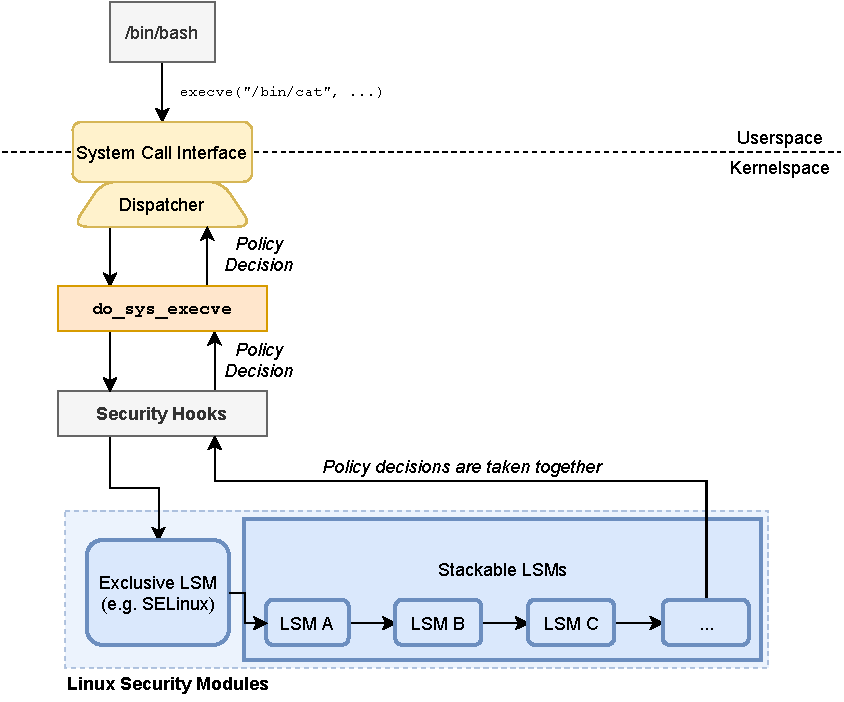
\includegraphics[width=0.8\linewidth]{figs/background/lsm.pdf}
  \caption[The LSM architecture]{
    The \gls{lsm} architecture. A single \textit{exclusive} \gls{lsm} may be loaded at a time,
    and complemented by zero or more \textit{stackable} \gls{lsm}s. When userspace
    requests a privileged operation (e.g.~through a system call), this operation causes one
    or more security hooks to be invoked. These hooks in turn call into the respective
    hook implementations provided by each loaded \gls{lsm}. Each hook returns a policy
    decision, and these decisions are then taken together to arrive at a final decision.
  }%
  \label{fig:lsm}
\end{figure}

After the introduction of the \gls{lsm} framework, SELinux was refactored into a Linux
security module~\cite{smalley2001_selinux} and subsequently merged into the mainline
kernel. SELinux supports three major types of mandatory access control: (i) role-based
access controls; (ii) type enforcement; and (iii) an optional \gls{mls} policy.
Fundamentally, SELinux policies are based on a notion of subject and object labelling.
A security policy assigns a specific label to subjects and objects, and then specifies
access patterns between these labels.

In an effort to simplify the SELinux policy language, a \textit{reference policy} was
introduced by PeBenito in 2006~\cite{pebenito2006_refpol}, providing a framework for
creating and managing reusable policy templates which can be integrated into new and
existing security policies. SELinux reference policies can be augmented with boolean
options, called \textit{tunables} that provide coarse-grained control over policy
behaviour to system administrators. Sniffen~\cite{sniffen06_guided} implemented a guided
policy generation system that walks application authors through the process of writing
SELinux policy. This framework was further augmented by
MacMillan~\cite{macmillan07_madison}, culminating in the eventual introduction of the
\texttt{audit2allow}~\cite{audit2allow} command line utility for automated policy
generation. Despite these usability improvements, the SELinux policy language is generally
considered to be quite arcane~\cite{schreuders2012_towards}, rendering it difficult for
non-expert users to write and audit security policy.

Since the introduction of SELinux, several alternative \gls{lsm}s have been proposed, many
of which have subsequently been merged into the mainline Linux kernel. AppArmor
(originally called SubDomain)~\cite{cowan2000_apparmor} takes an alternative approach to
SELinux, enforcing security policy based on \textit{pathnames} rather than security
labels.  AppArmor policies, called \textit{profiles}, are assigned on a per-executable
basis. Rather than being labelled, AppArmor policies identify system objects directly
(e.g.~through pathnames, \gls{ipc} categories, or network \gls{ip} addresses). Each system
object is associated with a particular access pattern, which determines the privileges for
a given AppArmor profile. Similar to SELinux, AppArmor offers a suite of userspace tooling
for automated and semi-automated policy generation based on enforcement
logs~\cite{aa_easyprof, aa_genprof, aa_logprof}.

\subsubsection*{Alternative Linux Security Modules}

Recognizing usability issues in the complexity of SELinux and AppArmor policies,
Schaufler~\cite{schaufler_smack} introduced SMACK (Simplified Mandatory Access Control
Kernel) to offer a simplified label-based enforcement scheme that focuses on expressing
a minimal set of permissions. Like SELinux, SMACK relies on labelling filesystem objects
using extended filesystem attributes. Policies then attach simple access specifiers to
these labels, based on canonical Unix permissions like \texttt{read}, \texttt{write}, and
\texttt{execute}. Some default labels are provided, which grant or revoke blanket
permissions for common tasks such as system daemons or the \texttt{init} process.

Schreuders \etal~\cite{schreuders2012_towards} designed FBAC-LSM (Functionality-Based
Access Control \gls{lsm}) with a similar goal of simplifying policy definition. Unlike
SMACK, which is based on labelling, FBAC-LSM specifies policy in terms of desired
\textit{functionality}. Specifically, FBAC-LSM policies define a set of high-level
functionalities that an application should exhibit. All other functionalities are
prohibited. Schreuders \etal~evaluated FBAC-LSM in terms of its usability and found that
it compares favourably against AppArmor and SELinux~\cite{schreuders2012_towards}.

Hu \etal~\cite{hu2013_fsf} proposed FSF (File System Firewall), which applies
firewall-like semantics to filesystem objects. Their goal was to create a more usable,
file-specific access control mechanism. FSF policies are defined in policy files,
comprised of simple rules that specify a file along with some combination of
\texttt{read}, \texttt{write}, and \texttt{execute} access. \textit{Redirection rules} are
primary differentiating factor between FSF and conventional file-based access controls.
Taking inspiration from similar functionality in network firewalls, a redirection rule can
be used to convert one file access into another, transparently to the target application.
Hu \etal~conducted a user study comparing their prototype to Unix \gls{dac} and SELinux
and found that FSF performed favourably in policy comprehensibility and accuracy.

The TOMOYO~\cite{harada2004_tomoyo} \gls{lsm} takes an alternative approach, emphasizing
policy generation and building generation functionality into the \gls{lsm} directly.
Rather than involving userspace helpers, TOMOYO generates policy by inferring
per-application profiles through the \gls{lsm} hooks they invoke. Programs can
additionally discard their privileges through a TOMOYO-specific system call, similar to
the notion of dropping privileges under the POSIX capabilities model. Like AppArmor,
TOMOYO relies on pathnames to identify resources rather than assigning security labels.
Users have the option to edit generated policies as required, but the intent is to require
as little user involvement as possible~\cite{harada2004_tomoyo}.

The Landlock~\cite{salaun_landlockio, salaun_landlock_patch} \gls{lsm} was recently
introduced into the mainline Linux kernel as a contemporary alternative to
\texttt{seccomp(2)} (covered in \Cref{sss:seccomp}). Landlock was originally intended to
allow unprivileged userspace processes to load highly restricted \gls{ebpf} programs into
the kernel to define security filtering logic~\cite{salaun_landlock_patch}. However, due
to concerns related to the security of unprivileged \gls{ebpf}, this functionality was
later reworked into a set of simple access rules and no longer has any association with
\gls{ebpf}~\cite{salaun_landlockio}. Under Landlock, a process creates a \textit{ruleset}
using the \texttt{landlock\_create\_ruleset(2)} system call, adds rules to that ruleset,
then confines itself by committing to that ruleset. Developers may add this confinement
logic directly into their software or may write specialized userspace wrappers to apply
generic confinement to applications.

Singh~\cite{singh2019_krsi} introduced the KRSI (Kernel Runtime Security Instrumentation)
framework for attaching \gls{ebpf} programs to \gls{lsm} hooks with the goal of defining
dynamic audit and policy enforcement filters. While similar in spirit to the original
Landlock proposal~\cite{salaun_landlock_patch}, KRSI differs fundamentally in that it
remains a \textit{privileged} \gls{lsm}; only root-privileged processes may load
\gls{ebpf} \gls{lsm} programs into the kernel. \bpfcontain{} and \bpfbox{} are both based
on the KRSI framework. \Cref{ss:bpf-programs-bg} examines the KRSI framework in more
detail.

%Radhakrishnan~\cite{radhakrishnan2006_kernelsec} \todo{DESCRIBE THIS OR DROP IT}



\subsection{System Call Filtering and Capabilities}%
\label{ss:syscall-filtering}

Since system calls define the canonical interface for communication between userspace
processes and the operating system kernel~\cite{jaeger2008_os_security}, they are
a natural fit for defining the protection interface of a confinement mechanism. In
particular, \textit{system call filtering} is a widely-used technique for application
sandboxing and self-confinement~\cite{anderson2017_comparison}. Indeed, \gls{lsm}s,
covered in the previous section, can be thought of as a form of system call filtering,
although security hooks are placed manually within system call implementations and do not
necessarily conform to the same semantics as the underlying system
calls~\cite{wright2002_lsm}.

Related to this notion of system call filtering are \textit{capabilities}\footnote{Here,
the term \enquote{capabilities} is a disparate term from \enquote{POSIX capabilities,} covered in
\Cref{ss:dac}.}, which guard access to a particular reference, associating privileges with
a handle to a given object on the system. For instance, the \texttt{open(2)} system call
returns a \textit{file descriptor}, which constitutes a reference to a particular
filesystem object. A capability associated with this file descriptor would then restrict
subsequent operations on the file descriptor, effectively restricting access to the
underlying file.

\subsubsection*{System Call Tracing}
\label{sss:ptrace}

In Unix, ptrace~\cite{ptrace, padala2002_ptrace} (short for process trace) is a mechanism
provided by the kernel that allows one process (the tracer) to attach itself to another
(the tracee), tracing and possibly manipulating nearly any aspect of its execution, system
calls, memory, and registers. Originally designed as a debugging interface~\cite{ptrace,
padala2002_ptrace}, ptrace has also been applied to implement system call
filtering~\cite{goldberg96_janus, wagner1999_janus, jain2000_filtering}. However, ptrace
has fallen out of favour, particularly in production use cases, due to its immensely high
overhead (on the order of several thousand percent~\cite{zinke2009_overhead}) and
propensity to introduce undefined behaviour when tracing even moderately complex
software~\cite{swiecki2017_promises}. Due to its invasive nature, a tracer process must
either be the direct parent of a tracee or must have sufficient privileges to trace the
child process\,---\,on Linux, this translates to either the \texttt{CAP\_SYS\_PTRACE}
capability or the all-encompassing \texttt{CAP\_SYS\_ADMIN}.

Janus~\cite{goldberg96_janus, wagner1999_janus} was an early exploration of how
\texttt{ptrace} could be applied to confine applications by filtering system calls.  The
original Janus prototype was designed for Oracle Solaris using its ptrace interface,
exposed through the \texttt{procfs} virtual filesystem~\cite{goldberg96_janus}.
A subsequent port of Janus was released for Linux~\cite{wagner1999_janus}, although it
required invasive modifications to Linux's ptrace implementation, dubbed ptrace++ by the
authors. Janus worked by attaching to the target process using ptrace, then tracing system
calls made by the target process and categorizing them into groups based on functionality.
A Janus policy could allow or deny specific categories of system call, confining the
application in a coarse-grained manner. The tracer process, called the \textit{supervisor
process}, would then be able to kill the offending process or inject failure into the
offending system call when it detected a policy violation.  Jain and
Sekar~\cite{jain2000_filtering} implemented a similar system call monitor, adding the
ability to modify system call arguments and using a different policy language design.

Provos' Systrace~\cite{provos2003_systrace} uses ptrace to analyze per-process system
calls and generate a system-call-level policy. Unlike Janus~\cite{goldberg96_janus,
wagner1999_janus} and Jain~\etal~\cite{jain2000_filtering}, Systrace supports intrusion
detection, policy generation, and audit logging, providing a mechanism to automatically
analyze process behaviour. Systrace also supports one highly unconventional feature, which
Provos calls \textit{privilege elevation}. The notion behind privilege elevation is to
allow a program to escalate its privileges selectively for specific system call access
patterns, preventing the need for coarse-grained privilege escalation such as setuid root.

Forrest, Somayaji, and Hofmeyr~\cite{forrest1996_sense_of_self} implement an intrusion
detection system, pH (process Homeostasis), based on system call sequences, although it
does not rely on ptrace and analyzes system call sequences instead of individual call
patterns. Rather than as a confinement solution, pH was strictly designed as a behavioural
anomaly detection system, although this approaches confinement as profile accuracy
improves.  Findlay~\cite{findlay2020_ebph} (the author of this thesis) later ported pH to
use \gls{ebpf} to analyze system call sequences.

\subsubsection*{OpenBSD Pledge and Unveil}
\label{sss:pledge}

OpenBSD's \texttt{pledge(2)} and \texttt{unveil(2)} system calls form the backbone of its
built-in sandboxing framework. A pledge~\cite{pledge} consists of a list of
\textit{promises}, high-level descriptions of what behaviours a program expects to exhibit
in the future, similar in spirit to Janus' high-level categories~\cite{goldberg96_janus,
wagner1999_janus}. The pledge system call takes two space-separated lists of promises, one
to be applied immediately and another to be applied upon making an \texttt{execve(2)}
call. To prevent privilege escalation, subsequent calls to \texttt{pledge(2)} take the
union of existing promises and new promises, precluding a process from escaping its
initial bounding set~\cite{pledge}.

Promises vary in granularity; the most coarse-grained promise, \texttt{stdio}, allows
a total of 69 distinct system calls, enabling the full suite of C standard library
stdio-family calls. Others, like \texttt{chown}, are more conservative, enabling only one
(albeit in this case very powerful) system call. In total, \texttt{pledge(2)} includes 33
distinct promises, as of OpenBSD 6.9~\cite{pledge}. Due to its coarse granularity and lack
of concern for specific system objects, pledge has been criticized as being
overly-permissive~\cite{anderson2017_comparison}.

Unlike pledge, \texttt{unveil(2)}~\cite{unveil, corbet2018_unveil} operates on specific
filesystem paths, making a promise about the kinds of operations the process will perform
on file descriptors associated with these paths. Specifically, unveil is concerned with
four kinds of permissions: read, write, execute, and create/delete. Unveiling a directory
unveils all files and directories underneath, recursively. Although this approach is
finer-grained than pledge, it is file-specific and offers a trade-off between granularity
and usability. The official manual page for unveil~\cite{unveil} recommends that
developers use it at the granularity of directories, despite the fact that this may result
in overpermission in practice. For instance, consider a hard link to the root of the
filesystem placed by an attacker within some unveiled directory. The unveiling process
would now have full access to the entire filesystem, constituting a sandbox escape.

\subsubsection*{Linux Seccomp and Seccomp-bpf}%
\label{sss:seccomp}

In Linux, the primary facility for direct system call filtering is
\texttt{seccomp(2)}~\cite{anderson2017_comparison, seccomp, prctl, edge2015_seccomp}.
Unlike OpenBSD's pledge and unveil~\cite{pledge, unveil}, seccomp filters directly over
system calls, without any blanket categorization. Initially, seccomp was highly limited,
restricting a process to only four system calls: \texttt{read(2)} and \texttt{write(2)}
for reading and writing open file descriptors, \texttt{sigreturn(2)} for handling signals,
and \texttt{exit(2)} to enable self-termination. Using any other system call would result
in an immediate SIGKILL delivered from the kernel, forcefully ending the offending
process.

Later, seccomp was extended to enable processes to define custom allowlists, denylists,
and enforcement actions using classic \gls{bpf} filters~\cite{edge2015_seccomp}. This new
incarnation was dubbed seccomp-bpf. While allowing for much finer-grained confinement
policy than pledge and unveil, seccomp-bpf has its own limitations which can result in
ineffective (and possibly dangerous) policies. In seccomp-bpf, filters are defined over
system call numbers and (optionally) arguments. Unless the developer takes great care to
correlate system call numbers with the specific target architecture, the resulting policy
may allow and deny incorrect system calls, resulting in broken policies that break
applications in the best case and expose security vulnerabilities in the worst case.

Another innate problem with seccomp arises due to its fine-granularity. Paradoxically,
avoiding system call categorization can expose vulnerabilities, due to system call
equivalence classes. For instance, the \texttt{openat(2)} system call can perform the same
functionality as the \texttt{open(2)} system call, with slightly different \gls{api} semantics.
A seccomp-bpf filter allowing one system call but denying the other is now totally broken
and vulnerable to sandbox escape.  Similarly, argument checking on pathnames or file
descriptors can be vulnerable to \gls{toctou} race conditions in practice, rendering such
policies ineffective~\cite{anderson2017_comparison}.

A final consideration for seccomp-bpf is that the development of seccomp-bpf policies
requires knowledge of the relatively arcane \gls{cbpf} syntax. This problem is somewhat
alleviated by the existence of library wrappers~\cite{libseccomp} around seccomp-bpf
functionality, although the usability of these solutions remains somewhat questionable,
particularly given the many pitfalls of seccomp-bpf policy
authorship~\cite{anderson2017_comparison}.

\subsubsection*{FreeBSD Capsicum and CHERI Capabilities}
\label{sss:capsicum}

Unlike the system call filters presented earlier in this section, FreeBSD's
\texttt{capsicum(2)} \cite{watson2010_capsicum, anderson2017_comparison} is a true
implementation of capabilities as they were originally described by Dennis and Van
Horn~\cite{dennis1966_semantics}. Specifically, capsicum capabilities are an extension on
top of Unix file descriptors, the canonical reference to files and file-like objects such
as network sockets and character devices. Capsicum adds an unforgeable access token to
each file descriptor, granting the corresponding process specific access rights over that
file descriptor. Whereas alternatives like seccomp-bpf~\cite{seccomp} and
pledge~\cite{pledge} restrict access at the system-call-level, capsicum restricts access
at the resource-level and enforces this access within the system call layer.

To confine processes, capsicum exposes a special \texttt{cap\_enter(2)} system call which
causes a process to enter \textit{capability mode}. A process in capability mode no longer
has access to global namespaces (e.g.~the PID namespace) and may only make a subset of
system calls which do not directly access these global namespaces. Other system calls are
constrained so that they may only operate under the context of an open capability
descriptor (a file descriptor which has been extended with capability
information)~\cite{watson2010_capsicum}. The end-result is an expressive and fine-grained
self-confinement framework for FreeBSD applications, which comes at a small usability cost
compared with coarser-grained alternatives like \texttt{pledge(2)}~\cite{pledge}.

In 2015, Watson \etal~designed CHERI~\cite{watson2015_cheri} as an extension to the MIPS
\gls{isa} enabling the capability-based protection of memory pages. Under CHERI, the
operating system kernel and userspace runtime extend the traditional memory model with
capabilities using the CHERI \gls{isa}. This enables generic capability-based protection at
the level of memory pages. While powerful, this extension requires dedicated hardware
support. Watson \etal~implemented their prototype on an \gls{fpga}~\cite{watson2015_cheri}
and later extended the FreeBSD \gls{abi} to work with CHERI capabilities~\cite{davis2019_cheriabi}.



\subsection{Taint Tracking}%
\label{ss:taint-tracking}

\textit{Taint tracking}~\cite{livshits2012_dynamic} describes the notion of tracking
changes to memory containing application data as it is mutated, copied, and moved by the
underlying application. Such data is considered \textit{tainted} when it is modified by
some external source in such a way as the data can no longer be trusted.  For instance,
a buffer might be populated by an external network connection or local user input. The
security benefits of such a mechanism are obvious. An active attack requires some user
input into a program in order to exploit a vulnerability; by tracking untrusted user input
and treating it as untrusted, developers can avoid attacker exploitation of sensitive code
paths. Beginning with Perl's \textit{taint mode}~\cite{hurst2004_perl}, taint tracking has
enjoyed a rich body of literature~\cite{livshits2012_dynamic, conti2010_taint,
bello2012_taint, ermolinskiy2010_towards, zavou2011_taint, yin2007_panorama,
zhu2011_taint_eraser, cheng2006_taint, clause2007_taint, chin2009_efficient} since its
inception.

In Perl's taint mode~\cite{hurst2004_perl}, a special command line flag triggers the
interpreter to flag untrusted user input and prevent it from being passed as input to
functions explicitly marked as \textit{unsafe}. To circumvent this restriction,
a developer could perform a pre-determined set of sanity checks on the data to
\textit{untaint} it. Rather than acting as an outright security mechanism, the goal was to
encourage developers to take care in processing untrusted data. Incorrect or insufficient
sanity checks on the data or running the Perl interpreter without the taint flag would
result in no additional security benefits whatsoever. After Perl, similar taint tracking
mechanisms have been added to other interpreters and language runtimes, including Ruby,
PHP, and Python~\cite{conti2010_taint}.

Conti, Bello, and Russo~\cite{conti2010_taint, bello2012_taint} implemented more advanced
taint tracking functionality for the Python programming language as a library that
developers could use directly. Their argument was that implementing such a taint mechanism
at the language-level rather than at the interpreter-level could enrich the traditional
taint-tracking approach with use-case-specific metadata and facilitate extensions to
support complex data types.

With the goal of creating a generic and reusable taint tracking mechanism, several
researchers have proposed application-transparent taint tracking. Many have turned to
virtualization or emulation runtimes~\cite{ermolinskiy2010_towards, zavou2011_taint,
yin2007_panorama} such as QEMU, KVM, or Xen, using built-in introspection features to
track the propagation of data within (and even between) running processes. Others have
proposed the adoption of static analysis or library
instrumentation~\cite{zhu2011_taint_eraser, cheng2006_taint, clause2007_taint} techniques
to reduce overhead and eliminate the need to run applications under expensive
virtualization monitors. Others have built taint tracking logic into existing language
runtimes, such as the Java Virtual Machine~\cite{chin2009_efficient}.



\section{Process-Level Virtualization}%
\label{s:virtualization}

We now step away from \textit{confinement} to focus on process-level
\textit{virtualization} primitives employed in Unix-like operating systems. Whereas
confinement primitives have the goal of restricting a process' behaviour, virtualization
primitives instead limit the process' ability to see the world around it. This property
should not be confused with \textit{isolation}. True isolation requires a mixture of both
virtualization and confinement mechanisms to restrict access to system resources and
prevent unwanted behaviour.

\subsubsection*{Chroots and Chroot Jails}

To virtualize the filesystem, Unix has classically supported the \texttt{chroot(2)} system
call~\cite{mcfearin2011_chroot_jails}, used to change the filesystem root (\texttt{'/'})
to some directory, specified as an argument. From the process' point of view, this
directory becomes its new filesystem root. However, chroot suffers from several issues
that render it totally ineffective as a security mechanism. Chroot escapes, path
traversals, spurious access to special filesystems and devices, and superuser privileges
all totally invalidate chroot as an isolation mechanism~\cite{mcfearin2011_chroot_jails}.

For instance, consider a call to \texttt{chroot("/my/new/root")}. Without a follow-up call
to \texttt{chdir(2)} to change the process' current working directory, a simple call to
\texttt{chdir("..")} is enough to escape the chroot jail. Even with the aforementioned
precautions, a process that has or is able to obtain superuser privileges can simply
create a new directory, re-invoke chroot, and perform the same escape as
before~\cite{mcfearin2011_chroot_jails}. Without the proper confinement mechanisms and
necessary precautions to prevent such escapes, chroot cannot be considered an effective
isolation technique. In fact, chroot escapes have been a source of many vulnerabilities
with container management engines like Docker in the past~\cite{combe2016_to_docker}.
McFearin~\cite{mcfearin2011_chroot_jails} proposed updates to the POSIX standard that fix
many of chroot's security flaws, but these have not been adopted.

\subsubsection*{FreeBSD Jails and Solaris Zones}

Kamp \etal~\cite{kamp2000_jails} presented FreeBSD's \texttt{jail(2)} as a more secure
alternative to \texttt{chroot(2)} jails. In particular, the jail system call is a heavily
extended wrapper around FreeBSD's chroot implementation. A call to jail begins by
allocating and populating a \texttt{prison} data structure that maintains metadata related
to the jailed process group, and finishes by simply invoking the standard chroot
implementation. Unlike chroot, Jails take care to avoid the standard pitfalls that may
result in a chroot escape and heavily limit the privileges of the root user within the
jail. In this respect, the jail system call can be seen as a hybrid between
a virtualization and confinement mechanism, approaching a full solution.

Jails take the approach of defining a clear security boundary around a collection of
processes, filesystem resources, and network resources~\cite{kamp2000_jails}. A process
existing within this boundary (i.e.~a member of the jail) enjoys the standard set of Unix
permissions on resources within the jail. Access to resources outside of the jail is
forbidden, including access by the root user. Visibility is similarly restricted by
remapping namespaces in such a way as outside resources are effectively invisible.
Defining a clear protection boundary enables the jail to enforce sensible security policy
without burdening the administrator with the details of writing such
a policy~\cite{kamp2000_jails}.

Solaris Zones~\cite{price2004_zones} later arose as a commercial solution for
process-level virtualization. The goal was to implement namespace remapping and security
isolation for commercial server deployments in (possibly multi-tenant) Solaris
environments. The implementation details of Solaris' Zones are similar to those of
FreeBSD's Jails; a per-task data structure manages the associate between tasks and Zones,
allowing the kernel to perform the necessary remapping and security checks.

\subsubsection*{Linux Namespaces and Cgroups}

Unlike FreeBSD~\cite{kamp2000_jails} and Solaris~\cite{price2004_zones}, Linux takes
a different approach to process-level virtualization. In particular, Linux's
virtualization strategy consists of two separate mechanisms, \textit{namespaces} and
\textit{cgroups} (short for process control groups). These mechanisms, in turn, can be
further subdivided into specific types, targeting different kinds of system resources.
Notably, namespaces and cgroups are \textit{not} confinement mechanisms in and of
themselves. This property is in stark contrast with Jails and Zones, which were designed
to offer strong confinement guarantees over their respective security boundaries.
As the canonical process-level virtualization building blocks in Linux, namespaces and
cgroups form the backbone of Linux containers (c.f.~\Cref{s:container-security-bg}).

Linux namespaces~\cite{biederman2006_namespaces, linux_namespaces} limit the visibility of
system resource by providing a virtual remapping of global resource identifiers to
a process or process group. Such identifiers include process IDs, user IDs, filesystem
mounts, IPC objects, and network interfaces, among others. Linux supports namespace
creation and entry via the \texttt{clone(2)} and \texttt{unshare(2)} system calls, for
isolating child processes and existing processes respectively. As of version 5.13, the
Linux kernel supports eight distinct namespaces, depicted in \Cref{tab:namespaces}. Other
namespaces have been proposed and/or planned for inclusion, including a security
namespace~\cite{sun2018_security_namespace} for virtualizing \gls{lsm} hooks.

\begin{table}
\begin{tabular}{lp{3in}}
    \toprule
    Namespace & Isolates \\
    \midrule
    \multirow{1}{*}{PID} & Process IDs (PIDs)\\
    \multirow{1}{*}{Mount} & Filesystem mountpoints\\
    \multirow{1}{*}{Network} & Networking stack\\
    \multirow{1}{*}{UTS} & Host and domain names\\
    \multirow{1}{*}{IPC} & Inter-process communication objects\\
    \multirow{1}{*}{User} & User IDs (UIDs) and group IDs (GIDs)\\
    \multirow{1}{*}{Time} & System time\\
    \multirow{1}{*}{Cgroup} & Cgroup membership\\
    \bottomrule
\end{tabular}
\caption[Linux namespaces]{
  Linux namespaces (as of kernel version 5.13) and what they can be used to isolate~\cite{linux_namespaces}.
}
\label{tab:namespaces}
\end{table}

Complementary to namespaces, cgroups~\cite{cgroups, gao2019_houdini} divide processes into hierarchical
groups, performing resource accounting and restricting access to quantifiable resources
such as memory, CPU clock cycles, block I/O, and device drivers. From a security
perspective, such restrictions are useful to prevent resource starvation attacks against
the host. However, Gao \etal~\cite{gao2019_houdini} found that this protection is
incomplete and often misleading, allowing up to 200$\times$ the allotted resource limits
by exploiting out-of-band resource consumption techniques. To interact with the cgroup hierarchy,
Linux exposes a virtual filesystem which encodes cgroup membership in its directory structure.
Cgroup membership visibility can be virtualized using the cgroup namespace~\cite{cgroups}.



\section{Containers and Virtual Machines}%
\label{s:containers-bg}

%This section introduces the concept of containers, examines how they compare with
%alternatives like hypervisor-based virtual machines, discusses the area of container
%security, and surveys related work in the container security space.

Classically, virtualization of a system has been accomplished by means of
a hypervisor~\cite{eder2016_hypervisor_container, sultan2019_container_security}.
Hypervisors implement an interface which overlays the underlying system hardware,
enabling one or more \textit{guest operating systems} to be installed on a single physical
host. These guest systems are then called \textit{virtual machines}. Due to the level of
indirection provided by the hypervisor and the guest operating system kernel, virtual
machines are generally considered to be quite \textit{strongly isolated} from each other,
but this isolation comes at the cost of much higher overhead, both in terms of storage and
performance~\cite{eder2016_hypervisor_container, sultan2019_container_security}.
\Cref{s:cp-rethinking} in \Cref{c:confinement-problem} discusses the differences between
virtual machines and containers in more detail and addresses some common misconceptions
about the levels of isolation they provide.

%Hypervisors can be classified into one of two types, depending on how they are deployed
%and implemented.  Type I hypervisors are implemented directly on top of hardware, whereas
%type II hypervisors run on top of a host operating system. This results in a further layer
%of indirection between the guest and the system hardware and thus a further degradation in
%performance.

% \todo{With HVMs, the security comes from the virtualization, well-defined barrier from one
% machine to another, opt in to whatever is going to cross it}

\textit{Containers} have emerged as a new unit of computation in recent years, providing
a lighter-weight alternative to full hypervisor-based
virtualization~\cite{sultan2019_container_security, eder2016_hypervisor_container}.
Unlike virtual machines, containers run directly on the host operating system, rather than
directly atop a hypervisor, and share the host operating system kernel with each other and
with ordinary host processes. In fact, a container is nothing more than a discrete
collection of processes (sometimes only one process) that share some common isolation from
the rest of the system by way of virtualization and confinement primitives. These
primitives typically include namespaces and cgroups, along with optional confinement
mechanisms like seccomp-\gls{bpf} and Linux \gls{mac} policy. Since they directly share
the host \gls{os} kernel and do not require a guest operating system, containers are
significantly lighter-weight and more performant than virtual machines, but at the cost of
weaker base isolation. \Cref{fig:virt} depicts the major differences between container and
hypervisor-based architectures.

% \begin{figure}[tbp]
%   \centering
%   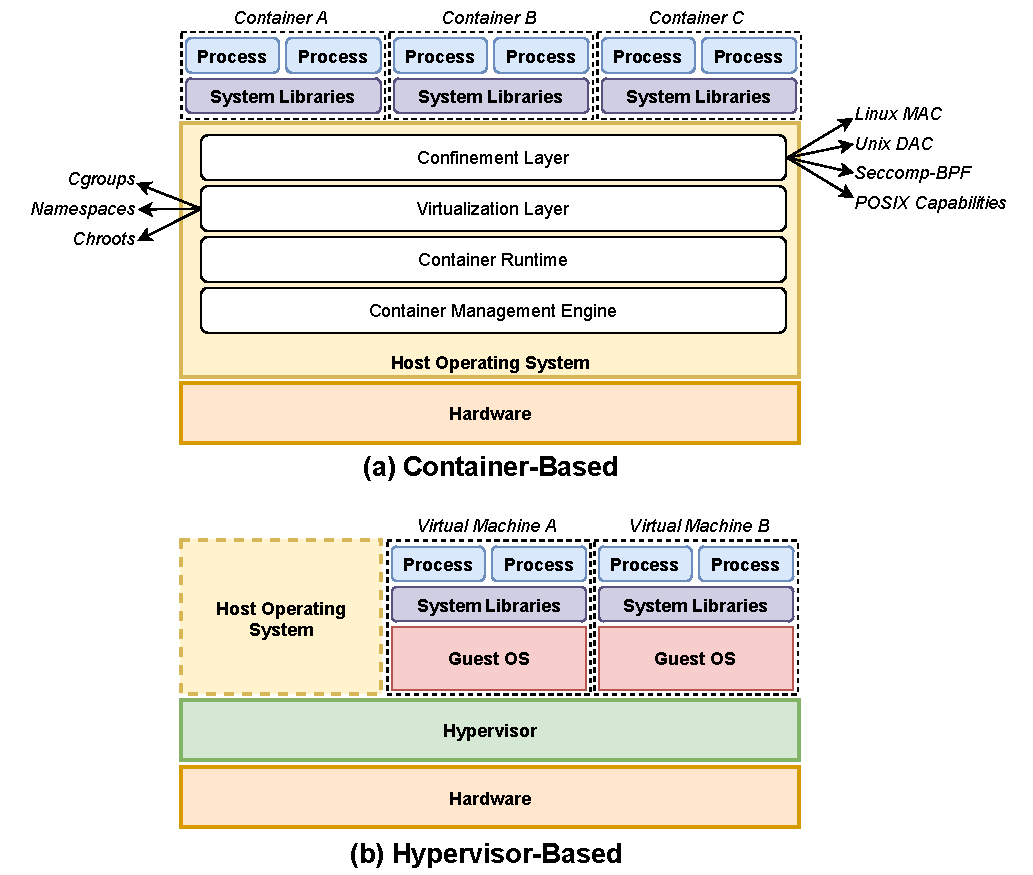
\includegraphics[width=0.8\linewidth]{figs/background/virtualization.pdf}
%   \caption[A comparison of virtual machine and container architectures]{
%     A comparison of virtual machine and container
%     architectures~\cite{sultan2019_container_security, eder2016_hypervisor_container}.
%     Containers \textbf{(a)} achieve virtualization using a thin layer provided by the host
%     \gls{os} itself. They share the underlying operating system kernel and resources,
%     requiring no guest \gls{os}. Type I hypervisors \textbf{(b)} virtualize and control
%     the underlying hardware directly, but require full guest operating systems on top of
%     the virtualization layer. Type II hypervisors \textbf{(c)} run on top of a host
%     operating system but still require full guest operating systems above the
%     virtualization layer.
%   }%
%   \label{fig:virt}
% \end{figure}

\begin{figure}[htbp]
  \centering
  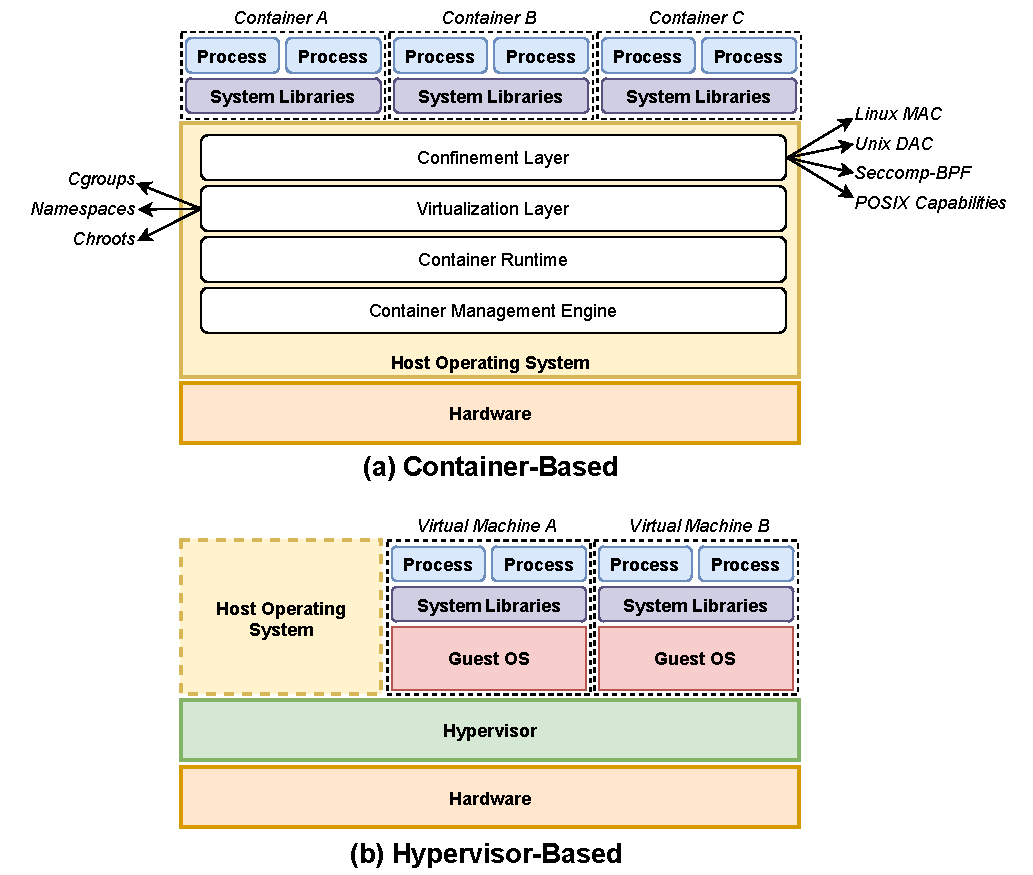
\includegraphics[width=1\linewidth]{figs/background/virtualization.pdf}
  \caption[A comparison of virtual machine and container architectures]{
    A comparison of virtual machine and container
    architectures~\cite{sultan2019_container_security, eder2016_hypervisor_container}.
    Containers \textbf{(a)} achieve virtualization using a thin layer provided by the host
    \gls{os} itself. They share the underlying operating system kernel and resources,
    requiring no guest \gls{os}. A hypervisor \textbf{(b)} virtualizes and controls the
    underlying hardware directly, but requires full guest operating systems on top of the
    virtualization layer.
  }%
  \label{fig:virt}
\end{figure}

% \begin{table}[htbp]
%   \centering
%   \caption[A high-level comparison of hypervisors and containers]{
%     A high-level comparison of hypervisors and containers. \fullc{} means property fully
%     satisfied; \halfc{} means property somewhat satisfied; and \emptyc{} means property
%     not satisfied.
%   }%
%   \label{tab:virt-comparison}
%   \begin{tabular}{lllcccp{1.6em}}
%   \toprule
%   & Deployment & Implementation & \rot{60}{1.6em}{Host-Isolated} & \rot{60}{1.6em}{Light-Weight} & \rot{60}{1.6em}{High-Performance} & \\
%   \midrule
%   Type I \glsentryshort{vm}  & Hardware & Guest \glsentryshort{os} & \fullc  & \halfc  & \halfc  & \\
%   Type II \glsentryshort{vm} & Host OS  & Guest \glsentryshort{os} & \halfc  & \emptyc & \emptyc & \\
%   Containers                 & Host OS  & Namespaces + Cgroups     & \emptyc & \fullc  & \fullc  & \\
%   \bottomrule
%   \end{tabular}
% \end{table}

\subsection{Container Security}%
\label{ss:container-security-bg}

Due to the nature of containers as specialized process groups, any notion of container
security is necessarily tightly coupled with the underlying security primitives exposed by
the host operating system. These include the virtualization primitives discussed in
\Cref{s:virtualization}, and the confinement primitives discussed in
\Cref{s:process-security-model,s:security-extensions}. Whereas the primary attack surface
of a virtual machine is comprised of the interface exposed on top of hardware, the attack
surface of a container is comprised of the system calls that it uses to interact with the
host operating system kernel. Every system call is an opportunity to exploit a kernel
vulnerability; over-zealous resource-sharing is an opportunity to establish a covert
channel, or perform a confused deputy attack~\cite{hardy1988_confused_deputy} against
a privileged application. The cost to mount such attacks rapidly decreases as isolation
from the host operating system decreases.

% While containers are lighter-weight than virtual machines, they are necessarily less
% secure, since they share and interact directly with the host operating system kernel.
% Although hypervisor escapes are not unheard of~\cite{dubrelle2015_hypervisor,
% eder2016_hypervisor_container}, they are far less common than container escapes,
% particularly given the fact that variabilities in container configuration can easily
% introduce holes in confinement~\cite{sultan2019_container_security}. Rather than going
% through a hypervisor (either directly to hardware or to a subsequent system call),
% containers directly make system calls to the host kernel. Not only does this make the
% probability of container escape more likely, but it also increases the host-to-container
% and container-to-host attack surface.

\Cref{fig:containersec} depicts a high-level threat model for containers from the
perspective of the host operating system. \todo{Connect each part of the figure to the
text.} This model comprises a number of attack vectors, each targeting a different part of
the system. A malicious container can target another container, a regular host process, or
the host operating system kernel. Similarly, a malicious host process can target
a container. To attack the \gls{os} kernel, a container must generally exploit
a kernel-level vulnerability, such as a memory safety error in a system call
implementation. To mitigate such attacks, the attack surface exposed by the kernel to the
container should be minimal. Other classes of attack rely on exploiting the intended
effects of system calls for in unintended ways.  For instance, a misconfigured security
policy might allow a containerized process to load a kernel module or perform interprocess
communication with an external daemon. Abusing shared resources can have a similar affect,
allowing a container to manipulate or tamper with an external process.

\begin{figure}[htbp]
  \centering
  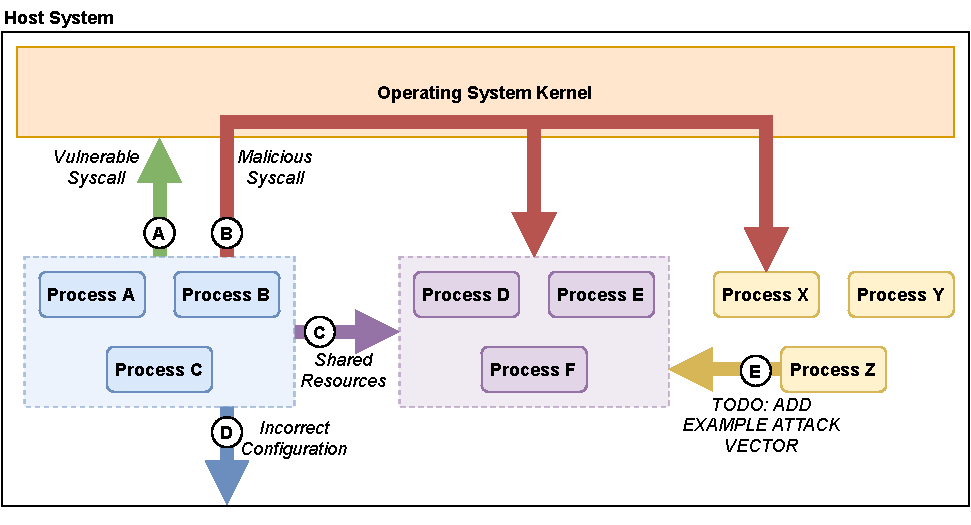
\includegraphics[width=0.8\linewidth]{figs/background/container_security.pdf}
  \caption[A sample threat model for container security]{
    A sample threat model for container security.
    \todo{Description here}
  }%
  \label{fig:containersec}
\end{figure}

\todo{Add a bulleted list of container escapes}
\begin{inprogress}
\begin{itemize}
  \item It's kind of leaky
  \item Even if you configure it perfectly, there are ways to misconfigure it
  \item The things you are subject to are the things you're subject to in the classic security model
  \item No different than software security in general... Because a container is just a set of processes
\end{itemize}
  \begin{itemize}
    \item Shared-resource attack
    \item Privilege escalation
    \begin{itemize}
      \item Exploiting a privileged process (e.g.~confused deputy)
      \item Exploiting kernel directly
    \end{itemize}
  \end{itemize}
\end{inprogress}

\subsubsection{Container Security in Industry}%
\label{sss:container-security-industry}

Existing container security on Linux is supported by a number of fundamental
virtualization and confinement mechanisms, covered in \Cref{s:process-security-model} and
\Cref{s:security-extensions}. Namespaces virtualize and limit the visibility of global
resource identifiers and cgroups virtualize and limit the available quantities of system
resources. Dropped POSIX capabilities allow the container to partition coarse-grained root
privileges into finer components. Seccomp-bpf filters limit the availability of system
calls to the container, while Linux \gls{mac} policies, enforced by an \gls{lsm} restrict
the container's access to system resources. Unix \gls{dac}, possibly accompanied by a new
user namespace, can limit the container's access as well, when properly configured.

\gls{lxc}~\cite{lxc_security} is a container runtime for Linux that directly exposes
low-level virtualization and confinement primitives. \gls{lxc} exposes namespaces and
cgroups to virtualize system resources and seccomp-bpf to filter system calls, reducing
the kernel's attack surface.

Docker~\cite{docker_security, bui2015_docker_analysis, combe2016_to_docker}, originally
based on \gls{lxc}, provides a high-level interface for creating, manipulating, and
running container images. Docker places containers in a new cgroup with sensible defaults
for resource virtualization. To isolate processes, the filesytem, and network interfaces,
Docker containers run in a new \texttt{pid}, \texttt{ipc}, \texttt{mnt}, and \texttt{net}
namespace by default.  Similarly, Docker uses the \texttt{uts} namespace for hostname
virtualization and the \texttt{cgroup} namespace to limit cgroup membership visibility. To
reduce the kernel's attack surface, Docker also includes a default seccomp-bpf profile
that blocks 51 system calls. Finally, Docker supports integration with the AppArmor
\gls{lsm} when it is enabled on the host, using a generic default profile that provides
modest protection~\cite{docker_apparmor, docker_default_apparmor}.

Unfortunately, Docker does not run in a new user namespace by default, making privilege
escalation from within a container significantly more likely~\cite{docker_security}.
However, it does offer the ability to opt-in to user namespace confinement with some
additional setup.  Docker also provides a \texttt{--privileged} flag which allows a user
to totally ignore all security defaults, essentially granting the container the same
access as a (often root-privileged) host process.

% \todo{Possibly discuss others: OpenVZ, OpenShift, more? Only talk in detail if they do
% something different}
% \todo{Possibly discuss containerized package managers: Snap, FlatPak, \etal?}
% \todo{be explicit about why we need}

\subsubsection{Container Security in Academia}%
\label{sss:container-security-academia}

Sultan \etal~\cite{sultan2019_container_security} published a comprehensive review of
container security, including a threat model and comparison with full-virtualization
solutions like type I and type II hypervisors. Their work outlined four distinct cases and
presented a survey of existing security mechanisms targeting each case: (i)
a containerized attacking the container; (ii) a container attacking other containers;
(iii) a container attacking the host; and (iv) the host attacking a container. Their
recommendations included an increased adoption of trusted computing technologies to solve
case iv and that work towards a container-specific \gls{lsm} would be necessary to harden
against cases i--iii. \bpfcontain{}, one of the two research systems presented in this thesis,
represents a step towards such a container-specific \gls{lsm}.

Lin \etal~\cite{lin2018_container_security} presented a measurement study on container
security measures and attacks. They hand-crafted an exploit data set consisting of 233
exploits and used it to test the security defaults employed by Docker. Their findings
indicated that inter-dependence and mutual-influence among several disparate kernel
security mechanisms resulted in weaknesses in protection. Motivated by their findings,
they developed a simple kernel patch hardening the \texttt{commit\_creds()} function
against simple privilege escalation attacks mounted from containers.

Combe \etal~\cite{combe2016_to_docker} and Bui~\cite{bui2015_docker_analysis} presented
informal security analyses of Docker's default security configurations and Docker security
in general. Combe \etal~\cite{combe2016_to_docker} found that Docker configurations are
weak to supply-chain attacks involving malicious images and configurations on Docker Hub.
Additionally, they found that, while Docker's default configuration is relatively secure,
container misconfiguration, or the absence of security mechanisms such as AppArmor on the
host leaves the host vulnerable to attack. They also found that the default mandatory
access control policies employed by Docker were overly-permissive and far too generalized
to provide practical protection.

Bui~\cite{bui2015_docker_analysis} found that, while Docker does offer inadequate
protection against many sophisticated attacks, it still yielded security benefits over
running applications natively on the host. Bui recommends that containers be run under
virtual machines to add an additional layer of isolation from the host system. These
findings, however, demonstrate a lax attitude toward container security, opting to rely on
additional layers of indirection to provide real security guarantees and positing that at
least some protection is better than none at all.
Eder~\cite{eder2016_hypervisor_container} compared hypervisor- and container-based
virtualization and found that hypervisors are naturally more secure due to increased
levels of independence and isolation.

Babar \etal~\cite{babar2017_understanding}, and Mullinix
\etal~\cite{mullinix2020_security_measures} studied the container security mechanisms
underlying the Linux container infrastructure. Their findings separately indicate that
existing security mechanisms provided by the kernel are insufficient to offer full
protection from container vulnerabilities, particularly given the unique nature of the
attack surface exposed by the container running directly on the host operating system.

To address limitations imposed by container security defaults and alleviate concerns about
poor security practices in default configurations, many researchers have turned to
automatic policy generation~\cite{loukidis2018_dockersec, ghavamania2020_confine,
lei2017_speaker}.  Dockersec~\cite{loukidis2018_dockersec} uses a combination of static
analysis techniques on existing security profiles and a dynamic training process to
automatically infer AppArmor profiles for containers.  These inferred profiles provide
greater protection than the generic default profile since they are finer-grained and
tailored to the container's access patterns. In addition to generating \gls{mac} policy,
others have focused on generating seccomp-bpf policy to reduce the kernel's attack surface
from within a container. Confine~\cite{ghavamania2020_confine} uses static binary analysis
and library call instrumentation to generate seccomp-bpf policy for container images.
Their results showed that they were able to significantly reduce the attack surface for
kernel exploitation in many of the most popular Docker images.
SPEAKER~\cite{lei2017_speaker} partitions application containers into two distinct
phases\,---\,the setup and execution phase\,---\, and generates a unique seccomp-bpf
policy for each phase, enabling a tighter bound on confinement for each phase.

Others have focused on promoting self-confinement for containerized applications. Sun
\etal~\cite{sun2018_security_namespace} proposed the inclusion of a security namespace
into the kernel, allowing individual containers to load their own independent \gls{mac}
policy. This approach enables a clear separation of concerns between host policy and
container policy, and provides a clear path toward unprivileged self-confinement. The
approach is also generic enough to enable the use of alternative \gls{lsm}-based
confinement solutions on a per-container basis. \bpfcontain{}, for instance, might work
cooperatively with security namespaces for more efficient per-container confinement.

Vulnerability analysis of container images~\cite{shu2017_image_vuln, kwon2020_divds,
brady2020_docker_cloud} can be an effective technique for identifying weaknesses in
container deployments. Unlike policy generation, vulnerability analysis is a strictly
informative tool, allowing security experts to identify weaknesses in production
deployments and fix them. Shu \etal~\cite{shu2017_image_vuln} presented DIVA, a framework
for analyzing vulnerabilities in images deployed from Docker Hub. They aggregated data
from over 350,000 container images and found that images contained an average of 180
security vulnerabilities. Kwon and Lee~\cite{kwon2020_divds} proposed DIVDS, which
extends prior work by providing an interface to compare and allow specific image
vulnerabilities.  Brady \etal~\cite{brady2020_docker_cloud} applied similar vulnerability
scanning techniques to a continuous integration pipeline, flagging and fixing image
vulnerabilities during development.

\gls{ebpf} is seeing increasing prominence within the container security space. Besides
\bpfbox{} (c.f.~\Cref{c:bpfbox}) and \bpfcontain{} (c.f.~\Cref{c:bpfcontain}), other
projects have arisen over the past few years, albeit with a general focus on observability
rather than policy enforcement. Tracee~\cite{tracee} is a container observability tool
developed by Aqua Security that can watch system calls made by a container, along with
other security-sensitive events, and generate audit logs for further analysis.
Cilium~\cite{cilium} is a popular security daemon for the Kubernetes container
orchestration framework, with a focus on network security for distributed container
deployments. Cilium provides observability metrics through a configurable audit framework
and allows the end-user to define network policy for telemetry, performance optimization,
and security.

\section{Extended BPF}%
\label{s:ebpf-bg}

\gls{ebpf} stands for \enquote{Extended \gls{bpf}}, though in reality it has very
little to do with Berkeley, packets, or filtering in its current
form~\cite{gregg2019_bpf}. In a nutshell, \gls{ebpf} is a Linux kernel technology that supports
dynamic system monitoring through the attachment of special \enquote{hooks} called \gls{bpf}
programs to specific kernel interfaces and userspace functions. In recent years, \gls{ebpf}'s
role has expanded, providing an interface to make extensions to the kernel as well as the
classic monitoring use case. In this section, we discuss the origins of \gls{ebpf}, its
components and how they work, its applications under the Linux kernel, and how it has
evolved over time.

\subsection{Origins of BPF\@: Efficient Packet Filtering and Beyond}%
\label{ss:origins-of-bpf-bg}

The original Berkeley Packet Filter, hereafter referred to as \gls{cbpf}\footnote{%
Throughout the rest of this thesis, we refer to extended \gls{bpf} using the terms
\enquote{\gls{ebpf}} and \enquote{\gls{bpf}} interchangeably. This is a matter of established
convention within the \gls{ebpf} community. Classic \gls{bpf} will be explicitly referred to by its
full name or the \gls{cbpf} acronym.}, arose out of a need to implement a more efficient packet
filtering mechanism for BSD Unix.  McCanne and Jacobson~\cite{mccanne1993_bpf} published
their work on \gls{cbpf} in 1993, marking an improvement over existing mechanisms in a number of
ways. Many of the reasons why classic \gls{bpf} was such an improvement over the status quo are
still relevant when discussing \textit{\gls{ebpf}}, and so we will briefly cover them here as
well.

In essence, classic \gls{bpf} is a \textit{register virtual machine} designed to take packets as
input and produce \textit{filtering decisions} as output. These filtering decisions could
then used to make decisions about whether a packet should be passed down to a more complex
pipeline for further analysis. The key insight behind \gls{cbpf} is that these filtering
decisions could be made more efficiently in \textit{kernelspace}, the part of the
operating system that runs in protection ring 0\footnote{Code that runs in ring 0 is said
to run with \textit{supervisor privileges} and is able to access all system memory. Ring
0 is the highest level of memory protection provided by the CPU~\cite{jaeger2008_os_security}.}
and which is most commonly associated with any parts of the operating system that do not
run in \textit{userland} (i.e.~the context of an ordinary user process). This provides
a considerable performance advantage over conventional approaches to network monitoring.
A typical network monitor runs in \textit{userspace}, meaning that packets need to be
copied over from kernelspace before they can be properly analyzed. This is an expensive
operation, requiring several context switches and potentially sleeping in the event of
a page fault~\cite{mccanne1993_bpf}.  By applying filtering logic in the kernel, this
expensive copying could be skipped for packets that would be discarded or ignored by the
network monitor anyway.

\begin{figure}[htbp]
  \centering
  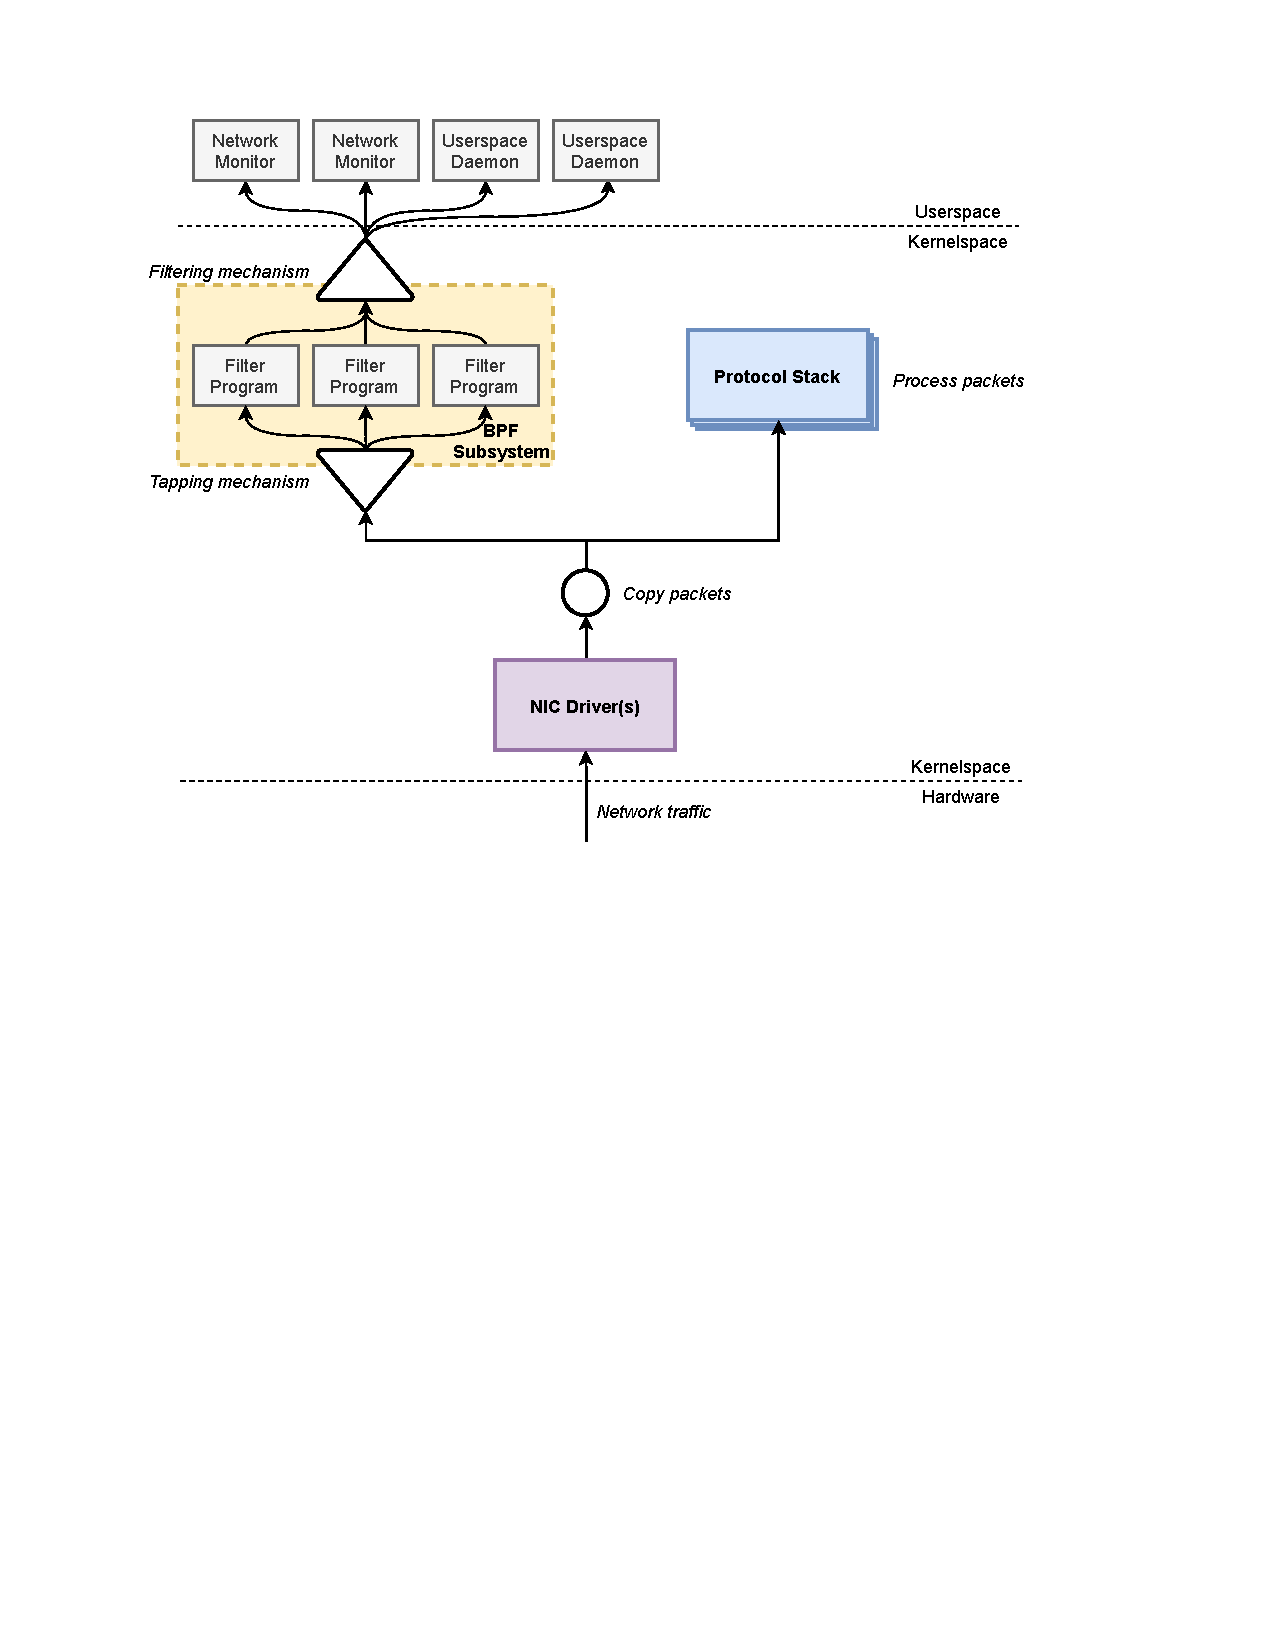
\includegraphics[width=0.8\linewidth]{figs/background/classic-bpf.pdf}
  \caption[The classic BPF architecture]{
    The classic \gls{bpf} architecture. Adapted from McCanne and Jacobson~\cite{mccanne1993_bpf}.
  }%
  \label{fig:classic-bpf}
\end{figure}

Classic \gls{bpf} can be divided into two major components: a \textit{tap} mechanism and a set
of one or more \textit{filter} programs. The cBPF architecture is depicted in
\Cref{fig:classic-bpf}. \gls{cbpf} programs are expressed as a control-flow graph (CFG)
over a set of abstract registers, backed by physical registers on the CPU. The tap
mechanism hooks into packets as they enter the networking stack, copying and forwarding
them to the filters. At runtime, the filter programs walk their control-flow graph, taking
the forwarded packets as input. As output, they return a filtering decision which controls
whether or not the packet should be forwarded to userspace~\cite{mccanne1993_bpf}.

Since its original introduction in 1993, classic \gls{bpf} has since been ported to
a number of Unix-like operating systems, including Linux~\cite{linux_bpf},
OpenBSD~\cite{openbsd_bpf}, and FreeBSD~\cite{freebsd_bpf}. Classic \gls{bpf} forms the
backbone of widely used traffic monitoring tools, most notably tcpdump~\cite{tcpdump,
mccanne1993_bpf}. In Linux, the \texttt{seccomp(2)} system
call~\cite{anderson2017_comparison} was enhanced to include classic \gls{bpf} filters,
allowing a user process to use classic \gls{bpf} programs to define allowlists and
denylists of system calls (c.f.~\Cref{sss:seccomp}).

In 2014, Alexei Starovoitov and Daniel Borkmann~\cite{starovoitov2014_ebpf} first proposed
a total overhaul of the Linux \gls{bpf} engine. Their proposal, dubbed \gls{ebpf}, expanded the
classic \gls{bpf} execution model into a full-fledged virtual instruction set. In particular,
the extensions included a 512 byte stack, 11 registers (10 of which are general-purpose),
the ability to call a set of allowlisted kernel helper functions, the ability to attach
programs to a variety of system events, specialized data structures (called \gls{bpf} maps) to
store and share data at runtime, and an in-kernel verification engine to check for program
safety. At runtime, programs can be dynamically attached to system events and are
just-in-time compiled into the native instruction set.  \Cref{fig:extended-bpf} depicts
the \gls{ebpf} architecture in detail. The reader is encouraged to compare this with the classic
BPF architecture, depicted in \Cref{fig:classic-bpf}.

Dtrace~\cite{cantrill2004_dtrace, gregg2001_dtrace} served as an early inspiration for the design of
\gls{ebpf} and related tooling. \todo{Say a bit more here.}

\begin{figure}[htbp]
  \centering
  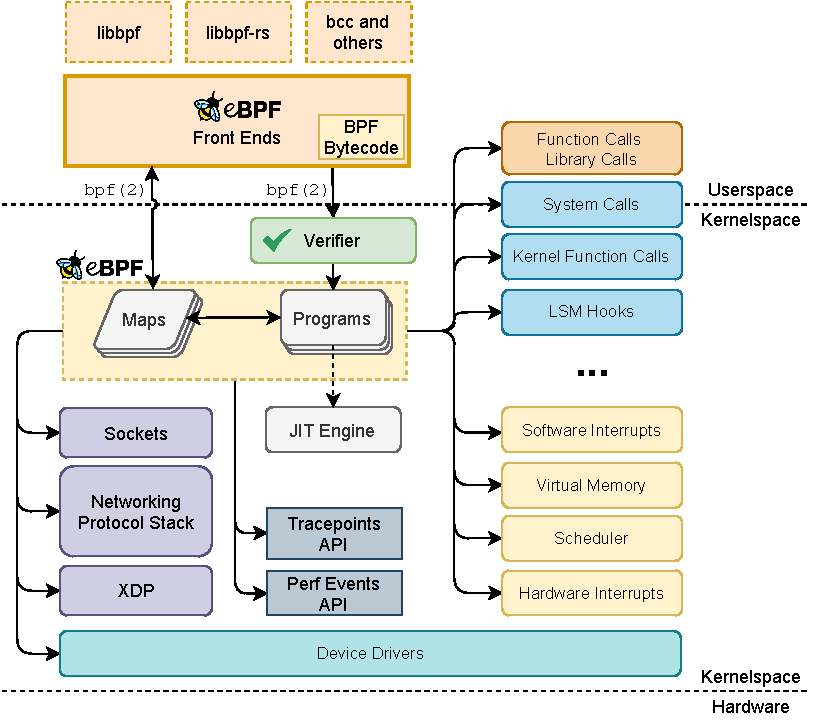
\includegraphics[width=0.8\linewidth]{figs/background/ebpf.pdf}
  \caption[The extended BPF architecture]{The extended \gls{bpf} architecture. Unlike classic
  \gls{bpf}, \gls{ebpf} programs are \gls{jit} compiled to the native instruction set, share data using
  specialized map data structures, and can be attached to many different kinds of system
  events. Programs can share data with each other and with the controlling userspace
  process using specialized map data structures. All \gls{ebpf} bytecode goes through
  a verification step before it can be loaded into the kernel.}%
  \label{fig:extended-bpf}
\end{figure}

While modern \gls{ebpf} has very little to do with the execution model of its older cousin, some
of the properties that made classic \gls{bpf} so performant still hold true today. In
particular, to notion of aggregating and processing data in kernelspace before
(optionally) handing it off to userspace is a key aspect of classic \gls{bpf} that has carried
over to \gls{ebpf}. What this means in practice is that \gls{ebpf} programs can be used to implement
very efficient monitoring software, harnessing the performance benefits of a pure
kernelspace implementation while maintaining the flexibility of a userspace
implementation.

\subsection{eBPF Programs}%
\label{ss:bpf-programs-bg}

\gls{ebpf} programs are expressed in a virtual RISC machine language called \gls{bpf} bytecode.  While
it is technically possible to write \gls{bpf} bytecode by hand, programs are most often compiled
from a restricted subset of the C programming language\footnote{Other languages may
eventually be used to write \gls{ebpf} programs as well.  For instance, an experimental \gls{ebpf}
target for the Rust programming language has recently been
proposed~\cite{decina2021_bpf_rust}. The important distinction here is that the set of all
possible \gls{ebpf} programs is a strict subset of the set of all possible programs.} using the
LLVM toolchain.Programs can be loaded and attached to system events using the
\texttt{bpf(2)} system call, at which point control passes to the \gls{ebpf} verifier, which
checks the programs to make sure they satisfy a set of safety
constraints~\cite{starovoitov2014_ebpf, gregg2019_bpf}.

In particular, \gls{ebpf} programs must consist of fewer than 1 million \gls{bpf}
instructions and must not call into any kernel functions outside of the allowlisted
helpers. The program is also constrained to a 512 byte stack size; any additional memory
required by the program must come from an \gls{ebpf} map (c.f.~\Cref{ss:bpf-maps-bg}). For
safety, memory accesses into allocated buffers must be properly bounds checked, pointers
must be null-checked before dereferencing, and any access to external memory
(e.g.~belonging to userspace programs or to the kernel itself) must be read-only. Since
\gls{ebpf} programs must provably terminate, no back-edges are permitted in their control
flow and all loops must be bounded by some fixed constant $i$ iterations.

To guard against data races, \gls{ebpf} programs always hold the kernel's RCU (read-copy-update)
lock while executing, gated by the \texttt{bpf\_prog\_enter} and \texttt{bpf\_prog\_exit}
functions in the kernel. In simple terms, the RCU lock allows concurrent reads, except in
the presence of updates, optimizing for read-mostly workloads (i.e.~precisely the sort of
workload \gls{ebpf} is designed for)~\cite{mckenney2007_rcu}. This implicitly enables \gls{bpf}
programs to read from many common kernel data structures without fear of data races and
simultaneously protects reads and updates to \gls{ebpf} maps, at a slight (albeit reasonable)
performance penalty~\cite{mckenney2007_rcu}. In addition to holding the RCU lock, \gls{ebpf}
programs are not considered \textit{preemptable} by default. In practice, this means that
\gls{ebpf} programs cannot sleep and must run to termination on their assigned core. This
property, while useful in many circumstances, enforces undesirable limitations on \gls{ebpf}
helpers, since it precludes any functionality that may cause the program to sleep (e.g.~a
page fault). To account for use cases where sleeping is unavoidable, Linux 5.10 introduced
sleepable versions of some \gls{ebpf} program types~\cite{starovoitov2020_sleepable}.

Once loaded into the kernel, \gls{ebpf} programs are represented as \gls{bpf} objects, each with its
own reference count. Loading a \gls{bpf} program and attaching it to a system event increments
the reference count, while detaching and unloading the program decrements the reference
count. The kernel also exposes a special filesystem, \textit{bpffs} , which allows \gls{bpf}
programs to be pinned. This also increments the reference count, allowing an attached
program to outlive its controlling process (i.e.~the process that loaded and attached
it)~\cite{gregg2019_bpf}.

\subsubsection*{Working with the Verifier}

In practice, the restrictions imposed by the verifier mean that \gls{ebpf} programs are not
\textit{Turing-complete}~\cite{gregg2019_bpf}.  This property is required, given that the
halting problem (i.e.~the decidability of program termination) is known not to be solvable
for Turing-complete programs. This notion of Turing-incompleteness means that the set of
all possible \gls{ebpf} programs is a strict subset of the set of all possible C programs. While
these limitations help to ensure program safety, they also naturally restrict some
operations which \textit{may} be safe but are not strictly verifiable. To overcome the
limitations imposed by the verifier and achieve this safe-yet-unverifiable behaviour, \gls{ebpf}
programmers have a few tools in their arsenal. For instance, a specific set of allowlisted
kernel helpers offers the ability to call into specific kernel functions, bypassing the
limitations imposed by the \gls{ebpf} verifier. As a simple example, the
\texttt{bpf\_probe\_write\_user()} helper allows an \gls{ebpf} program to write to a userspace
memory address, bypassing the read-only restrictions imposed by the verifier. While these
allowlisted helpers operate in a \textit{mostly} unrestricted context, their usage
\textit{is} restricted at the function call boundary, ensuring that the \gls{ebpf} program obeys
the safety contract specified by the helper function.  Another common design pattern is
using a dummy \gls{ebpf} map as a scratch buffer to reserve a larger amount of memory for the
\gls{ebpf} program.  Since \gls{ebpf} programs cannot sleep~\cite{gregg2019_bpf}, dynamic memory
allocation within the \gls{bpf} context is impossible. These dummy maps offer a way to access
additional memory from a pool reserved at the time the map was loaded into the kernel.

\subsubsection*{eBPF Program Types and Use Cases}

Each \gls{ebpf} program has a specific \textit{program type}, which determines both the set of
system events to which the program can attach and the set of allowed kernel helpers that
can be called from within the program context. Each program type roughly corresponds with
a distinct \gls{ebpf} use case. For the purposes of this thesis, we will primarily be dealing
with \textit{\gls{lsm} probes}, \textit{raw tracepoints}, \textit{fentry/fexit probes}, and
\textit{uprobes/uretprobes}, as they form the basis of \bpfbox{} and \bpfcontain{}'s
kernelspace implementations. \Cref{tab:program-types} summarizes the relevant program types
and their properties.

\begingroup\footnotesize
\begin{longtable}[c]{lp{4.2in}}
\caption[A selection of relevant eBPF program types for \bpfbox{} and \bpfcontain{}]{A selection of relevant \gls{ebpf} program types for \bpfbox{} and \bpfcontain{}.}%
\label{tab:program-types}\\
  \toprule
  Program Type & Description\\
  \midrule
  \textit{\gls{lsm} Probes}    & \gls{lsm} probes~\cite{singh2019_krsi} attach to the kernel's \gls{lsm} hooks and can be used to audit security events and make policy decisions.\\
  \textit{Raw Tracepoints}     & Raw tracepoint programs attach to a stable tracing interface exposed by the Linux kernel. Tracepoints are considered a stable \gls{api}, but are more limiting than alternatives such as Kprobes or Fentry probes.\\
  \textit{Kprobes/Kretprobes}  & Kprobe programs can attach to any kernel function, by replacing the function with a trap into the \gls{bpf} program. The \gls{bpf} program has read-only access to the function arguments. Kretprobes work in the same way, but handle function returns instead of function calls.\\
  \textit{Fentry/Fexit Probes} & A more efficient version of Kprobes and Kretprobes that directly trampolines into the \gls{bpf} program instead of trapping. These programs can also be used to modify the return value of specifically allowlisted kernel functions (e.g.~system call implementations).\\
  \textit{Uprobes/Uretprobes}  & The userspace equivalent of Kprobes and Kretprobes.\\
  \bottomrule
\end{longtable}
\endgroup

\subsubsection*{LSM Probes: Making Security Decisions with eBPF}

It is worth spending more time focusing specifically on \gls{lsm} probes, as these are used
extensively in \bpfbox{} and \bpfcontain{} to enforce policy over security-sensitive
events. Introduced by KP Singh in his \gls{krsi}
patch~\cite{singh2019_krsi}, \gls{lsm} probes define a canonical framework for attaching \gls{ebpf}
programs to the Linux kernel's \gls{lsm} security hooks (c.f.~\Cref{ss:mac}). Unlike
traditional \gls{lsm}s which are implemented as static kernel modules, \gls{lsm} probes are
\textit{dynamically attachable}, meaning that \gls{mac} and audit policy can be adjusted at
runtime, simply by loading a new \gls{ebpf} program.  \Cref{fig:bpf-lsm} depicts how \gls{lsm} probes
integrate with the \gls{lsm} framework.

\begin{figure}[htbp]
  \centering
  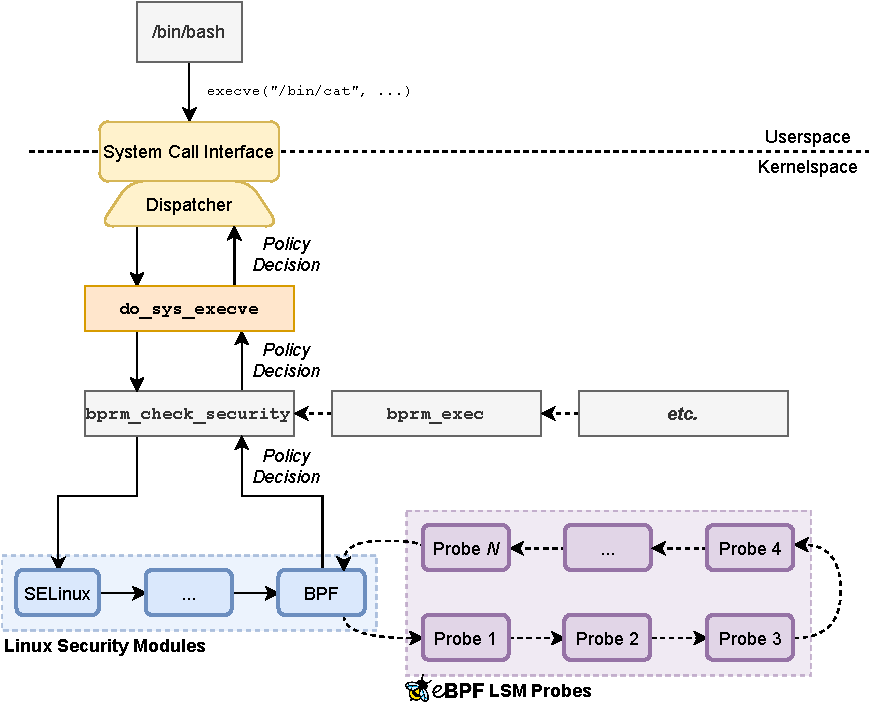
\includegraphics[width=0.8\linewidth]{figs/background/bpf-lsm.pdf}
  \caption[How eBPF LSM probes make policy decisions]{A simplified example of how \gls{ebpf} \gls{lsm} probes make policy decisions. Privileged userspace processes can attach one or more \gls{lsm} probes to a given hook. When a userspace process requests a privileged operation, the kernel implicitly calls into the corresponding \gls{lsm} hooks, which in turn invoke the logic associated with each \gls{lsm}. A shim \gls{lsm} is responsible for invoking each \gls{lsm} probe, and any resulting policy decisions are taken together to arrive at a final decision. As with ordinary \gls{lsm}s, the final decision is consensus-based. That is, if \textit{any \gls{lsm}s} or \textit{any \gls{bpf} \gls{lsm} probes} disagree on a policy decision, the privileged operation is denied.}%
  \label{fig:bpf-lsm}
\end{figure}

As with other \gls{lsm}s, \gls{lsm} probes implement a form of mandatory access control.
Each \gls{lsm} probe can be attached to one or more \gls{lsm} hooks defined in the kernel.
When the hook fires (i.e.~when a task requests a privileged operation form the kernel),
every attached probe fires as part of the normal \gls{lsm} pipeline. The body of the
\gls{bpf} program defines filtering and audit logic, optionally accessing maps to store
and query persistent state. The \gls{bpf} program then returns a security decision about
whether the requested operation should be allowed or denied.  In order for an operation to
be allowed, \textit{all} other \gls{lsm}s and \gls{lsm} probes must agree on the policy
decision and ordinary security checks performed by the operating system must also succeed.
In other words, it is not possible to grant additional privileges using an \gls{lsm}
probe.

Owing to the properties discussed earlier in this section, \gls{ebpf} confers a natural
flexibility to \gls{lsm} probes quite unlike that of traditional \gls{lsm}-based security
frameworks.  In particular, \gls{lsm} probes can be attached at runtime and can cooperate
with other \gls{ebpf} program types using \gls{ebpf} maps (c.f.~\Cref{ss:bpf-maps-bg}).
This notion of cooperating programs presents an opportunity to design modular policy
enforcement mechanisms that operate beyond the scope of the \gls{lsm} hooks framework
itself.  Another key advantage of \gls{lsm} probes over traditional \gls{lsm}s lies in
their adoptability.  While industry actors may be understandably reluctant to adopt
\enquote{yet another out-of-tree \gls{lsm}}, a security mechanism based on \gls{ebpf} does
not carry the same technical baggage.  \gls{ebpf} programs are safe to use in production
and can be deployed at runtime on an unmodified kernel.  This makes \gls{ebpf}
a particularly attractive target for developing new security solutions.

\subsection{eBPF Maps}%
\label{ss:bpf-maps-bg}

\gls{ebpf} maps serve as both a runtime data store for \gls{ebpf} programs and the
canonical method of communication between \gls{ebpf} programs and other \gls{ebpf}
programs, and \gls{ebpf} programs and userspace applications. Like \gls{ebpf} programs,
maps can be pinned to \textit{bpffs} to increment their reference count in the kernel.
Concurrent access to \gls{ebpf} maps from within kernelspace is protected by an implicit
RCU lock, and a spinlock concurrency primitive is exposed via a helper function to guard
map accesses between kernelspace and userspace.  From the \gls{ebpf} side, maps can be
accessed using a set of provided helper functions.  Userspace applications can access maps
using the \texttt{bpf(2)} system call or through direct memory-mapping (only available for
arrays) via \texttt{mmap(2)~\cite{gregg2019_bpf}}. While many \gls{ebpf} maps are designed
to be generic, others are highly specialized for specific use cases. \bpfcontain{} and
\bpfbox{} make use of several \gls{ebpf} map types, which are summarized in
\Cref{tab:map-types}.

\begingroup\footnotesize
\begin{longtable}[c]{lp{3.9in}}
\caption[A selection of relevant eBPF map types for \bpfbox{} and \bpfcontain{}]{A selection of relevant \gls{ebpf} map types for \bpfbox{} and \bpfcontain{}.}%
\label{tab:map-types}\\
  \toprule
  Map Type & Description\\
  \midrule
  \textit{\gls{bpf} Hashmap}           & A key-value hashmap. Keys and values can be arbitrary data structures.\\
  \textit{\gls{bpf} Array}             & A fixed-size array with integer indices. Values can be arbitrary data structures.\\
  \textit{\gls{bpf} Array/Map of Maps} & A \gls{bpf} array or map that stores handles into \textit{other maps}.\\
  \textit{\gls{bpf} Per-CPU Array/Map} & Like a \gls{bpf} hashmap or \gls{bpf} array but with a separate copy per logical CPU\@. This enables concurrent access across CPUs, but without synchronization.\\
  \textit{\gls{bpf} Local Storage}     & A dummy \gls{bpf} map that provides a handle into local storage for a given kernel data structure. For instance, task local storage provides storage per-task-struct. Values can be arbitrary data structures.\\
  \textit{\gls{bpf} Ringbuf}           & A concurrent circular buffer that passes event handles from kernelspace to userspace. To communicate, \gls{ebpf} programs submit events and userspace applications poll events.\\
  \bottomrule
\end{longtable}
\endgroup

\subsection{Userspace Front-Ends}%
\label{ss:bpf-userspace}

Although \gls{ebpf} programs and maps can exist on their own after being pinned to
\textit{bpffs}, the more common approach is to manage their lifetime using a controlling
process. Userspace applications implementing such a controlling process typically use an
\gls{ebpf} front-end framework to facilitate loading and interacting with programs and maps.
A number of such front-ends exist~\cite{gobpf, bcc, libbpf, libbpf-rs, libbpfgo,
cilium-ebpf, redbpf}, some more practical than others.
\textit{bcc}~\cite{bcc} was the first \gls{ebpf} framework to offer high-level userspace tooling
around \gls{ebpf}, providing an LLVM backend for compiling \gls{ebpf} programs and a Python library
for loading and interacting with them. \textit{libbpf}~\cite{libbpf} offers a pure
C alternative to bcc and has since been upstreamed into the Linux kernel.
\textit{libbpf-rs}~\cite{libbpf-rs} and \textit{libbpfgo}~\cite{libbpfgo} offer Rust
and Golang bindings for libbpf respectively. Other tooling~\cite{cilium-ebpf, redbpf}
bypasses libbpf entirely, providing fully native \gls{ebpf} bindings for Rust and Golang.

\subsubsection*{Libbpf and BPF CO-RE}%

Among the myriad of userspace front-ends available for \gls{ebpf}, libbpf stands out as the only
one with official upstream support from the Linux kernel. Recent improvements to libbpf
have solidified its position as the dominant framework. In particular, libbpf supports
a new way of compiling and loading \gls{bpf} programs into the kernel, \gls{bpf}
\gls{core}~\cite{gregg2020_core, nakryiko2020_core}. \gls{bpf} \gls{core} uses \gls{btf}
debugging information exposed by the kernel, along with load-time relocation logic to
support loading the same compiled \gls{ebpf} bytecode across multiple target kernels. The
precise technical details of how \gls{core} works are beyond the scope of this thesis.

With libbpf and \gls{core}, \gls{ebpf} programs can now be compiled once and run on any target kernel
that supports the required \gls{bpf} features. This provides a powerful advantage over other
\gls{ebpf} frameworks and even alternatives to \gls{ebpf}, such as loadable kernel modules. A \gls{core}
program that runs on one kernel will be guaranteed to run on another of the same version
or higher, barring any \gls{api} incompatibilities like changes in a hooker function signature.
Such incompatibilities can be resolved with the use of built-in kernel configuration
checks.

\bpfcontain{} (c.f.~\Cref{c:bpfcontain}) leverages libbpf and \gls{core} through libbpf-rs, the
canonical Rust bindings for libbpf, providing adoptability advantages over the original
\bpfbox{} prototype (c.f.~\Cref{c:bpfbox}), which uses bcc.

\subsection{Comparing eBPF with Loadable Kernel Modules}%
\label{ss:bpf-vs-modules}

Before \gls{ebpf}, the primary means of modifying the Linux kernel at runtime was through the
use of \textit{loadable kernel modules}~\cite{corbet1998_device_drivers}. A kernel module
can be thought of as a discrete bundle of code that can be loaded into the kernel (or
compiled into its binary image). Like other kernel code, including \gls{ebpf}, modules are
event-based and run in ring 0, responding to and handling system events as they occur.
Since kernel modules and \gls{ebpf} can serve similar (but not strictly equivalent) purposes,
comparing the two can offer some insight about how they differ and which technology is
better fit for a specific purpose.

At a first approximation, \gls{ebpf} differs from kernel modules in the following meaningful ways~\cite{gregg2019_bpf}:
\begin{enumerate}
  \item \gls{ebpf} programs \textbf{must pass verification checks} before they can be loaded into the
  kernel. This verification step provides assurances about program safety. For instance, \gls{ebpf}
  programs are guaranteed not to deadlock the kernel, and are far less likely to suffer from
  memory safety issues. In contrast, misuse of kernel \gls{api}s in a kernel module can have dangerous
  implications for system safety and security.

  \item An implicit advantage provided by \gls{ebpf} is that \gls{bpf} programs can be \textbf{easier
  to reason about} than other kernel code. \gls{ebpf} abstracts away much of the complex
  functionality required to make kernel code operate correctly by providing implicit
  guarantees about program execution. Even helper functions, which offer functionality
  beyond the scope of verifiability, must obey a predetermined contract with the verifier
  in order to be considered safe. Thus, when an \gls{ebpf} program passes verification, there is
  a much higher likelihood that it will \enquote{just work.}

  \item \gls{ebpf} \textbf{exposes map-like data structures} to facilitate runtime data storage,
  communication between \gls{ebpf} programs, and communication with userspace applications. In
  the case of kernel modules, data structures often must be implemented by hand, taking
  great care not to introduce potential bugs or security vulnerabilities, particularly in
  the case of memory management. Communication with userspace from a kernel module might
  be done via netlink sockets, file operations, or similar
  means~\cite{corbet1998_device_drivers}. These modes of communication are often less
  streamlined and, in the case of file operations, must be implemented by hand, increasing
  the likelihood of programmer error.

  \item \gls{ebpf} programs are \textbf{not Turing-complete}. Intuitively, this means that
  the set of operations a kernel module can perform is a strict superset of \gls{ebpf}. While
  this may appear to be a hugely limiting factor, in practice \gls{ebpf} programs are often
  sufficient to implement sophisticated tracing, filtering, and policy enforcement logic.
  Where the verifier gets in the way, the programmer can reach for a number of helper
  functions provided by the kernel to achieve more complex behaviour.

  \item \gls{ebpf} is \textbf{not suitable for implementing device drivers} or other complex
  functionality that requires ad-hoc access to various kernel facilities and write access
  to arbitrary memory locations.
\end{enumerate}

In summary, \gls{ebpf} is useful for observability use cases, or cases in which the functional
requirements of the kernel code are not expected to be complex or might be expected to
change frequently. \gls{ebpf} programs and maps are particularly good at separation of concerns,
composability, and modularity. \gls{ebpf} maps facilitate easy communication between kernelspace
and userspace, and provide the ability to build relationships between data from different
program types. Kernel modules should be preferred for the implementation of more complex
kernel functionality, such as device drivers.

\todo{A summary table here would be nice}


\chapter{The Confinement Problem}%
\label{c:confinement-problem}
\begin{inprogress}
Researchers have been studying confinement for decades~\cite{lampson1973_confinement}, and
have been designing and applying confinement primitives since the early days of
time-sharing computers and multi-tenant systems~\cite{shu2016_security_isolation_study}.
Despite decades of research into the confinement problem, the status quo of confinement on
Linux, particularly from the perspective of containers, is in a sorry state. This chapter
outlines the difficulties that arise in the Linux confinement ecosystem due to its
inherent complexity, inflexible and interdependent components, and the difficulties that
arise in adopting newly-proposed alternatives. These insights represent the key
motivating factors behind the design of \bpfbox{} and \bpfcontain{} and can potentially
inform the way we think about new confinement mechanisms going forward.
\end{inprogress}

\section{Rethinking the Virtualization Narrative}%
\label{s:rethinking-virtualization}

Hypervisor-backed virtualization is commonly considered more secure than container-based
virtualization~\cite{sultan2019_container_security, eder2016_hypervisor_container}.
Intuitively, this makes sense. Containers run directly on the host operating system,
whereas a virtual machine runs on top of a hypervisor, separated by at least one layer of
indirection from the host system. However, this intuition does not strictly stand up to
scrutiny. A virtual machine running on top of a hypervisor makes requests to the
hypervisor's \gls{api} (via hypercalls), in much the same way as a container running on
a host operating system makes requests to the kernel's \gls{api} (via system calls).
\Cref{fig:syscall-hypercall} illustrates this parity.

\begin{figure}[htbp]
  \centering
  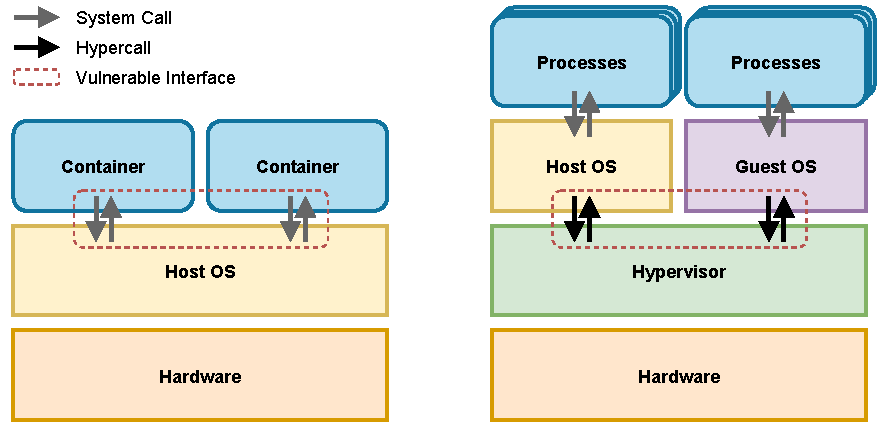
\includegraphics[width=0.8\linewidth]{figs/confinement-problem/syscall-hypercall.pdf}
  \caption[]{
    \todo{Caption here}
  }%
  \label{fig:syscall-hypercall}
\end{figure}

The isolation guarantees provided by a virtual machine come almost entirely from a sense
of obfuscation over a semantic gap, created as the hypervisor virtualizes system
resources.  There is no notion of centralized policy in a virtual machine; rather,
security is an emergent phenomenon, a form of \enquote{policy through mechanism}. With the
right tools, we can and have poked holes everywhere in this
policy~\cite{dubrelle2015_hypervisor, thongthua2016_analysis, shahzad2017_systematic}.

The central argument of this thesis is that there is no fundamental reason why containers
cannot be as\,---\,if not more\,---\,secure than virtual machines.
\begin{inprogress}
  \begin{itemize}
    \item The point is that we just need to define a clear protection boundary
    \item \bpfbox{} lays the foundation for this, and \bpfcontain{} brings it home
    \item In \bpfbox{} policies are defined in a centralized, flexible policy file, and
          integrate a variety of possible behaviours together in a simple and clear way
    \item In \bpfcontain{}, we build a container abstraction into \bpfbox{}, and use this
          to inform an \textit{implicit policy}. This defines a very clear boundary for
          operations that can impact the container vs operations that can impact the system as
          a whole. Behaviour \textit{within} the container is unrestricted, whereas behaviour
          that can impact the world outside the container is implicitly denied. Policy then
          defines \textit{exceptions} to this implicit policy, rather than \textit{rules}.
    \item The key insight is that \gls{ebpf} allows us to get this container abstraction
          in a flexible and adoptable way, rather than forcing it into the mainline kernel.
          Yet we still have the flexibility to incorporate various aspects of system state
          into our enforcement decisions, beyond simple \gls{lsm} hooks.
  \end{itemize}
\end{inprogress}

\begin{inprogress}
  \begin{itemize}
    \item To accomplish something like this, we need a way to define a single, clear,
          protection boundary into containers
    \item This requires a fundamental change in the way containers are handled on the kernel side
    \item Specifically, we need a good abstraction for containers in order to be able to enforce
          a clear and effective policy for then
    \item Lead into the next section: Given the existing state of confinement on Linux,
          this may not seem like a feasible task, but we assert that new kernel technologies
          are making this possible (i.e.~eBPF and \bpfbox{}/\bpfcontain{}).
  \end{itemize}
\end{inprogress}

\begin{inprogress}
  \begin{itemize}
    \item Just like the word container makes people think about security
    \item Type I and Type II hypervisor, the way it's depicted, makes people think something else is happening
    \item The representation and terminology
    \item This makes sense to talk about it if we connect it to containers
    \item Why can't containers give as good or better security than hypervisors
    \item Can we just get our enforcement clear
    \item Virtual machines seem like they define a clear boundary, but it isn't actually
          so clear in practice because all these things are being shared across boundaries
    \item People think of virtual machines as being inherently more secure, the security
          benefit is more of an obfuscation thing related to the semantic gap but with the right
          tools you can still cross it freely
    \item VMs have all these little holes everywhere and the policy is not centralized\,---\,we
          have policy through mechanism
    \item There's no reason why containers can't be as (if not more) secure than virtual machines
    \item Because we can make this boundary very clear
    \item \bpfcontain{} can be seen as a step towards this
  \end{itemize}
\end{inprogress}

\section{Fundamental Issues with Linux Confinement}%
\label{s:cp-confinement-issues}

\begin{enumerate}
  \item \textbf{Complexity and Interdependence.}
    Existing confinement primitives are overly complex and designed for use
    cases beyond simple process confinement. This results in a pattern of
    abusing existing mechanisms
  \begin{inprogress}
    \begin{itemize}
      \item Existing confinement solutions are overly complex
      \item Based on a number of low-level primitives that were originally designed for
            totally different tasks.
      \item Namespaces were designed to virtualize resources. They provide a form of
            isolation but not confinement; need a way to deal with namespace escapes
      \item Cgroups, similarly, were designed to virtualize the availability of system
            resources, not to directly confine.
      \item Unix \gls{dac} is far too coarse-grained and easy to bypass to be practically useful for confinement.
      \item POSIX capabilities can be used to reduce overprivilege by portioning root privileges, but do not
            implement confinement by themselves.
      \item Seccomp-bpf works well to reduce the availability of system calls, but writing
            classic \gls{bpf} filters is complex and error-prone. Anything beyond basic system call
            filtering quickly becomes untenable, particularly considering race conditions when
            checking arguments.
    \end{itemize}
  \end{inprogress}

  \item \textbf{Inappropriate Defaults.}
  \begin{inprogress}
    \begin{itemize}
      \item
    \end{itemize}
  \end{inprogress}

  \item \textbf{Difficulty Adopting New Solutions.}
  \begin{inprogress}
    \begin{itemize}
      \item Motivated by the above difficulties, academics are often tempted to propose new confinement solutions.
      \item Many try to solve the problem by simply recombining and reusing these existing primitives in new ways.
      \item This isn't really a step forward, as we are still subject to limitations introduced in item 1 and item 2.
      \item To really solve the problem, we need kernel-level support for something new.
      \item The issue is that new solutions based on kernel support are not necessarily
            adoptable. New kernel code can introduce bugs and security vulnerabilities, and
            needs to be thoroughly tested before it can be considered production-ready.
      \item Another problem arises when we consider container-specific confinement as an
            end goal; not everyone can agree on what the definition of a \enquote{container}
            even is, so how can we hope to reach agreement on what a new abstraction for
            container-based confinement would even look like.
      \item To solve this problem, we need a way to add new abstractions to the kernel in
            a way that is neither binding nor limited by the lack of adoptability associated
            with traditional kernel-based solutions.
    \end{itemize}
  \end{inprogress}
\end{enumerate}




\section{Confinement in Container Management Frameworks}%
\label{s:cp-containers}

\begin{inprogress}
Linux containers have three broad goals. In order of perceived prioritization in existing
container implementations, they are:
\begin{enumerate}
  \item \textbf{Dependency Management / Reproducibility.}
    Containers should provide an easy and robust framework for creating reproducible
    development environments. Dependencies should be maximally self-contained such that
    a containerized environment \enquote{just works} to the maximum possible extent. We
    can see examples of this property in Docker, the predominant container framework to
    date. Docker Hub~\cite{docker_hub} allows container images to be pulled from the
    Internet, recombined, and used to create further images. The end result is a flexible
    framework for creating and distributing reproducible development environments.

  \item \textbf{Virtualization.}
    Containers should virtualize system resources, creating the illusion of running on
    a separate physical machine. Where possible, resources should be transparently reused
    between multiple containers (e.g.~sharing a single base copy of the same shared
    library between two container images). To achieve virtualization, containers generally
    rely on the namespaces and cgroups primitives provided by the Linux kernel. Overlay
    filesystems~\cite{overlayfs} combined with the mount namespace aid containers one-way
    sharing of filesystem resources.

  \item \textbf{Confinement.}
    Containerized processes should be confined by default. That is, a containerized
    process should have access to the minimal set of privileges required for it to operate
    normally. The extent to which this property is achieved by conventional container
    frameworks varies greatly, both by framework and by individual
    deployment~\cite{sultan2019_container_security, lin2018_container_security,
    bui2015_docker_analysis}.
\end{enumerate}

Unfortunately, the aforementioned goals are not only ordered by their decreasing
prioritization in extant container management frameworks, but they are also ordered by
increasing relevance to container security. That is to say, existing frameworks generally
prioritize goals unrelated to security and leave security as an afterthought. Since
containers are necessarily less isolated from the host system than virtual
machines~\cite{sultan2019_container_security, eder2016_hypervisor_container}, one might
expect container security to be of paramount importance. This motivates the need to
revisit container security and approach it from a confinement-first perspective.
\end{inprogress}

\begin{inprogress}
  Container security policies are often overly-generic and ill-suited to fine-grained
  confinement. To achieve confinement in the first place, container frameworks cobble
  together existing confinement technologies and apply them in confusing and
  difficult-to-audit ways, overlapping and recombining default and generated policies. The
  end result is a complex security soup with little room for policy customization or
  auditability. \todo{Examples here}

  Even worse, many container management systems operate under a fail-open approach when the
  necessary security mechanisms are not supported. This results in low-security deployments,
  often without even notifying the user that there may be such a configuration. Since the
  end-user generally doesn't even participate in the policy authorship process, they may not
  even be aware of the level of protection that is being applied, resulting in a dangerous
  false sense of security. \todo{Examples here}
\end{inprogress}




\section{Design Goals}%
\label{s:design-goals}

Using the above analysis of the confinement problem, we can derive a clear set of design
goals for \bpfbox{} and \bpfcontain{}, such that they approach a solution to issues that
plague the status quo. In particular, we derive the following three design principles.
Note that these design principles are each the polar opposite of the three major problems
identified at the beginning of this chapter (c.f.~\Cref{s:cp-confinement-issues}).

\begin{enumerate}
  \item \textbf{Simplicity and Flexibility.}

  \item \textbf{Sensible Defaults.}

  \item \textbf{Adoptability.}
\end{enumerate}



\section{The \bpfbox{} and \bpfcontain{} Threat Model}%
\label{s:threat-model}


\chapter{\bpfbox: A Prototype Process Confinement Mechanism}%
\label{c:bpfbox}
This chapter presents the design and implementation of \bpfbox{}, an initial research
prototype of an \gls{ebpf}-based confinement framework. \bpfbox{} is the first
full-fledged confinement framework to leverage \gls{krsi}'s \gls{lsm} programs to enforce
high-level policy. Using \gls{ebpf}, it combines various behavioural aspects of the
sandboxed application from both userspace and kernelspace to enforce a simple, yet
fine-grained policy defined in a domain-specific policy language. This chapter was a part
of a previously published paper at CCSW'2020, co-authored with Anil Somayaji and David
Barrera~\cite{findlay2020_bpfbox}.



\section{\bpfbox{} Overview}

At a high level, \bpfbox{} is a confinement mechanism based on \gls{ebpf}. As outlined in
\Cref{s:cp-design} of \Cref{c:confinement-problem}, our primary design goals are
simplicity, flexibility, suitability for containerized applications, and flexibility. With
this in mind, \bpfbox{} attempts to be as light-weight as possible, with a simple policy
language that supports optional granularity. Perhaps the most important goal of \bpfbox{}
may be derived from the aforementioned goals: to make per-application security policy
accessible to end-users. To achieve these goals, we leverage \gls{ebpf} for \bpfbox{}'s
kernelspace implementation and rely on a number of its intrinsic properties.

In particular, we take advantage of multiple program and map types (outlined in
\Cref{ss:bpfbox-architecture}). This design enables us to trace multiple aspects of system
behaviour, including userspace and kernel function calls, and combine these with
\gls{lsm}-layer enforcement, thanks to the \gls{krsi} extension that enables \gls{bpf}
programs to be attached to \gls{lsm} hooks. By sharing data across program types in this
way, we enable \bpfbox{} to define extremely fine-grained \gls{lsm} policy at the
per-function-call level, something which no existing process confinement mechanism can do.

Since \gls{ebpf} programs may be loaded dynamically into a vanilla kernel and provide
implicit safety guarantees thanks to the verifier, we ensure that \bpfbox{} is both
light-weight and more adoptable than conventional solutions based in static \glspl{lsm}
like SELinux or AppArmor. Since all of \bpfbox{}'s kernelspace code is pre-verified, it is
also significantly less likely to adversely affect a production kernel than an alternative
solution implemented as a kernel patch or kernel module.

Whereas the kernelspace components are implemented using \gls{ebpf} programs written in C,
\bpfbox{}'s userspace components are implemented in Python3. In particular, this consists
of a privileged daemon loads \bpfbox{}'s \gls{ebpf} programs and maps into the kernel,
manages their lifecycle, and logs policy enforcement actions for later examination.

% This daemon is implemented in bcc~\cite{bcc}, a Python3 library that acts as
% a userspace \gls{ebpf} front-end.  bcc in turn is based on libbpf~\cite{libbpf} and uses
% the LLVM toolchain~\cite{llvm_bpf} to compile its \gls{bpf} programs at runtime before
% they can be loaded into the kernel.

\subsection{Policy Enforcement at a High Level}%
\label{ss:bpfbox-enforcement-overview}

To confine an application, a user first authors a high-level policy written in \bpfbox{}'s
domain-specific policy language (outlined in \Cref{s:bpfbox-policies}). The policy
language is designed in such a way as to permit the authorship of simple confinement
policies while offering the ability to augment them with specific context. Thus, the user
has full control over the balance between policy expressiveness and policy simplicity. We
expect that application authors may wish to take advantage of \bpfbox{}'s full
expressiveness, whereas end-users may wish to overlook advanced features in favour of
simple, light-weight confinement policy.

Once a policy has been written, the user places it in a pre-determined policy directory
and loads \texttt{bpfboxd}, the \bpfbox{} daemon. The daemon compiles and loads its
\gls{bpf} programs and maps into the kernel, then parses the user-supplied policy and
encodes it into policy maps. When a user launches the target application, \bpfbox{} begins
tracing the lifecycle of the corresponding processes and associates them with the correct
policy. As the application runs, \bpfbox{} continually updates security-critical aspects
of its state, stored in intermediary maps. As the application makes requests to sensitive
resources, \bpfbox{} queries policy maps and state maps and uses this information to come
to an enforcement decision. \Cref{fig:bpfbox-policy-overview} outlines this process in full.

\begin{figure}[htpb]
  \centering
  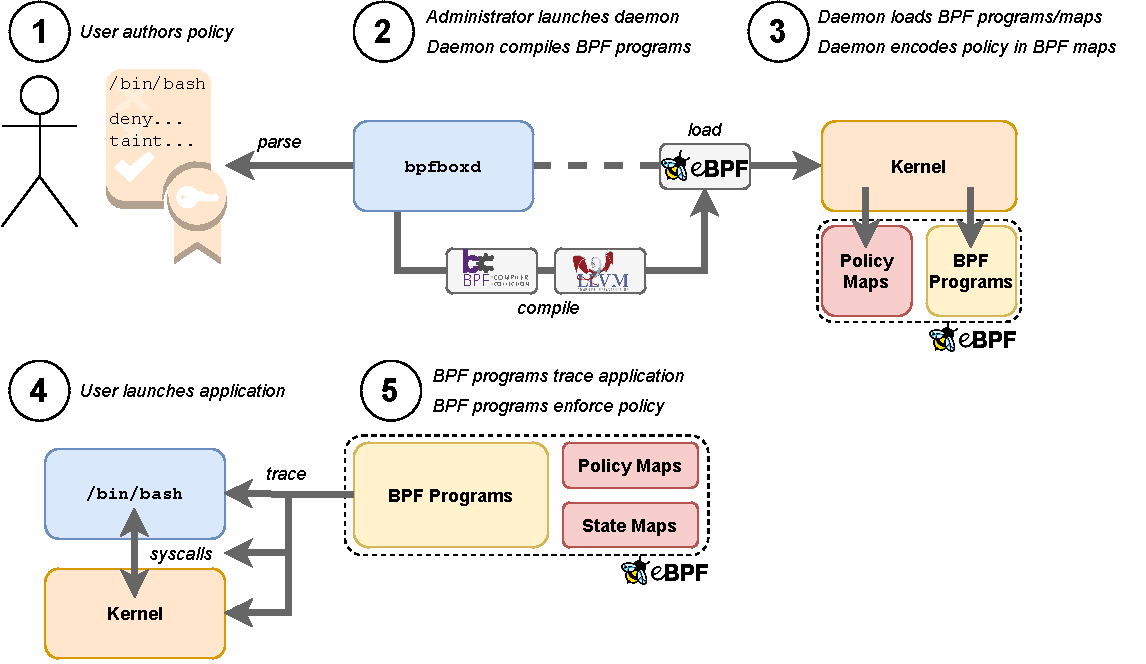
\includegraphics[width=0.8\linewidth]{figs/bpfbox/overview.pdf}
  \caption[A high-level overview of how \bpfbox{} confines applications]{
    A high-level overview of how \bpfbox{} confines applications. Users write policy files
    which the daemon encodes into \gls{ebpf} maps. The daemon loads these maps, along with
    policy enforcement and tracing programs into the kernel. At runtime, \bpfbox{}'s
    \gls{bpf} programs trace the application and enforce policy.
  }%
  \label{fig:bpfbox-policy-overview}
\end{figure}



\section{\bpfbox{} Implementation}%
\label{s:bpfbox-implementation}

This section presents the implementation details and full architecture of \bpfbox{}.  In
particular, we provide an architectural overview and discuss \bpfbox{}'s policy
enforcement implementation, along with how it tracks and manages the state and lifecycle
of sandboxed processes. We focus specifically on implementation details here, leaving
policy language design and documentation to \Cref{s:bpfbox-policies}.

\subsection{Architectural Overview}%
\label{ss:bpfbox-architecture}

In userspace, \bpfbox{} runs as a privileged daemon (\texttt{bpfboxd}), implemented in
Python3 using the bcc~\cite{bcc} userspace library for \gls{ebpf}. The daemon uses the
LLVM toolchain~\cite{llvm_bpf} to compile \gls{ebpf} programs which are then loaded into
the kernel using bcc-provided wrappers around the \texttt{bpf(2)} system call. The daemon
provides a userspace front-end to \bpfbox{}, managing the lifecycle of its \gls{bpf}
programs and maps and logging security-sensitive events as they occur. To load policy into
the kernel, \texttt{bpfboxd} implements a full parser and lexer for \bpfbox{}'s custom
policy language.  After parsing policy, \texttt{bpfboxd} encodes it into a format that can
be subsequently loaded into kernelspace through \gls{bpf} maps.

\bpfbox{}'s kernelspace components are implemented in \gls{ebpf} and based on several
\gls{bpf} program and map types, summarized as follows. Maps are outlined in
\textbf{\green{green}} and programs are outlined in \textbf{\purple{purple}}. The reader
is encouraged to revisit \Cref{ss:bpf-programs-bg,ss:bpf-maps-bg} in \Cref{c:background},
where necessary, for clarification on specific program and map types.

\begin{itemize}
  \item \bpfbox{} uses \textbf{\green{Hashmaps}} to store runtime state, share state
  between its \gls{bpf} programs, and communicate with the userspace daemon. In
  particular, \bpfbox{} maintains a set of hashmaps to store per-process state and a set
  of hashmaps to store policy. We call these \textit{state maps} and \textit{policy maps}
  respectively.  At runtime, \bpfbox{}'s \gls{lsm} programs query these state maps and
  policy maps to make enforcement decisions.

  \item \textbf{\green{Ringbufs}} provide \bpfbox{}'s \gls{bpf} programs with a canonical
  data store to push per-event audit data to userspace. In the kernel, the ringbuf map is
  implemented as a circular buffer that is efficiently shared across all \glspl{cpu}.
  In userspace, the \bpfbox{} daemon maps the ring buffer into memory and continually
  polls for new events over a fixed interval.
  % \item \textbf{State Maps} are \gls{ebpf} hash maps that associate a kernel \gls{tid}
  % with a specific task state. The task state holds information including policy
  % association, task liveness, and other metadata used for enforcement.

  % \item \textbf{Policy Maps} are \gls{ebpf} hash maps that encode \bpfbox{} policy for
  % various categories of access. Each map encodes an access vector and policy ID pair that
  % is mapped to the corresponding enforcement decision. At runtime, \bpfbox{} queries these
  % maps before making an enforcement decision on a specific access pattern.

  \item \textbf{\purple{Tracepoints}} enable \bpfbox{} to track the state of a process from the
  point where it forks or executes a new binary to when it exits. \bpfbox{} stores
  per-process state from its tracepoints in \textit{state maps} for later use.

  \item \textbf{\purple{\gls{lsm} Probes}} enforce policy by attaching to \gls{lsm} hooks in the
  kernel. These hooks are called by kernel functions such as system call implementations
  and trigger the corresponding \gls{bpf} program, which enforces a policy decision on the
  target application. To enforce policy, \bpfbox{}'s \gls{lsm} probes query \textit{policy
  maps} and \textit{state maps}.

  \item \textbf{\purple{Kprobes and Uprobes}} are used to enforce \textit{stateful policy},
  according to what function calls a process has made, in kernelspace and userspace
  respectively. A \bpfbox{} policy file may outline that certain rules should only apply
  within the context of a specific function call; when a process runs some code that
  results in such a function call, the corresponding kprobe or uprobe will make an update
  to the process' \textit{state map} to indicate this. \bpfbox{} then considers this state
  when making later enforcement decisions.

  \item \textbf{\purple{\gls{usdt} Probes}} form the backbone of \textit{libbpfbox},
  providing a kernel-side implementation for various \enquote{commands}. Commands are
  implemented in userspace as stub \gls{usdt} functions that trap to a kernelspace
  \gls{usdt} program. These are used to load policy into the kernel and perform various
  other interactions between the daemon and its \gls{bpf} programs and maps.
\end{itemize}

\subsection{\bpfbox{} Policy Enforcement}%
\label{ss:bpfbox-enforcement}

\bpfbox{} policies are written using a custom policy language.  \bpfbox{}'s policy
language supports three distinct policy decisions for a given rule; the operation may be
allowed, audited (logged), and/or tainted.  Any unspecified operations are denied by
default. Tainting is similar in spirit to Perl's classic taint mode~\cite{hurst2004_perl},
however, rather than marking data, it marks the entire process.  Tainting allows for more
restrictive policies to be enforced once a process has engaged in specific unsafe
operations, say by reading from a network socket.  We present the design and syntax of the
\bpfbox{} policy language in \Cref{s:bpfbox-policies}; here we discuss the functionality
it provides and how it is implemented.

\bpfbox{} policies are per-executable and are stored in an exclusively root-controlled
directory (by default, \texttt{/var/lib/bpfbox/}), written in \bpfbox{}'s policy language
(c.f.~\Cref{s:bpfbox-policies}). When an executable is loaded, \bpfbox{} loads the corresponding
policy file (if it exists) and translates it into a series of function calls to \gls{usdt}
stub functions.  These function calls trigger the corresponding \gls{ebpf} code, thus recording
the policy in the policy maps as a set of policy structures.  A policy structure consists
of three distinct access vectors: one to define tainting operations, one to define allowed
operations, and one to define audited operations.

In order to enforce policy, \bpfbox{} leverages the KRSI patch by KP
Singh~\cite{singh2019_krsi, corbet2019_krsi} which was upstreamed in Linux
5.7. This patch provides the necessary tools to implement MAC policies in \gls{ebpf} by
instrumenting probes on \gls{lsm} hooks provided by the kernel. The \gls{ebpf} program can then
audit the event and optionally enforce policy by returning a negative error value.
\bpfbox{} instruments several \gls{lsm} probes covering filesystem access, \gls{ipc}, network
sockets, \texttt{ptrace(2)}, and even \texttt{bpf(2)} itself.  When these hooks are
called in the kernel, they trigger the execution of the associated \gls{ebpf} program which
is, in general, composed of the following six steps:
\begin{enumerate}
\item Look up the current process state.  If no state is found, the process is
      not being traced, so \textbf{grant access}.
\item Determine the \textit{policy key} by taking the executable's inode
      number and filesystem device number together as a struct.
\item Look up the policy corresponding to the \textit{policy key} calculated in step (2). If the
      process is \textit{tainted} and no such policy exists, \textbf{deny access}.
\item If the process is \textit{not tainted} and the current access corresponds to
      a \textbf{taint rule}, \textbf{taint} the process and \textbf{grant access}.
\item If the current access matches an \textbf{allow rule}, \textbf{grant access}.
      Otherwise \textbf{deny access}.
\item If the current access matches an \textbf{audit rule} or access is \textbf{denied},
      submit an \textit{audit event} to userspace.
\end{enumerate}

%\Cref{fig:bpfbox-enforcement} depicts \bpfbox{}'s mediation of a request
%to a security-sensitive resource.

When a sandboxed application requests access, a corresponding \gls{lsm} hook is called which in
turn traps to one or more of \bpfbox{}'s \gls{lsm} probes. The probe queries the state of the
currently running process along with the policy corresponding to the requested access and
takes these factors together to come to a policy decision.

%% \begin{figure}[tpb]
%%     \centering
%%     \includegraphics[width=1\linewidth]{figs/bpfbox-enforcement.png}
%%     \caption{\bpfbox{}'s mediation of a security-sensitive operation.
%%     Security-sensitive operations by sandboxed applications trap to an
%%     \gls{lsm} hook which in turn invokes the corresponding BPF \gls{lsm} probe to
%%     query and enforce policy.
%%     }%
%%     \label{fig:bpfbox-enforcement}
%% \end{figure}

\bpfbox{} can optionally augment the information provided by the \gls{lsm} hooks themselves with
additional context obtained by instrumenting other aspects of process behaviour. For
instance, profiles may optionally define \textit{function contexts} which determine the
validity of specified rules; a rule could specify that a certain filesystem access must
occur within a call to the function \texttt{foo()} or that it must be audited within
a call to the function \texttt{bar()}. The ability to combine various aspects of system
behaviour, both in kernelspace and in userspace, is a key advantage of an \gls{ebpf}-based
solution over traditional techniques. This allows for the creation of extremely
fine-grained policies at the discretion of the policy author. The mechanisms by which this
is accomplished are discussed further in \Cref{ss:bpfbox-state}.

Due to \bpfbox{}'s strict resolution of filesystem objects at policy load time, a problem
arises when dealing with applications that read or write temporary files on disk or create
new files at runtime. In order to circumvent this issue, \bpfbox{} treats the creation of
new files as a special case. In order for a new file to be created, the process must have
write access to the directory in which the files will be created.  Supposing, for
instance, the temporary file would be written to \texttt{/tmp}, this means that, at
a minimum, the policy in question must specify that \texttt{/tmp} is writable.  When the
sandboxed application creates a new child inode of \texttt{/tmp}, \bpfbox{} dynamically
creates a temporary rule that grants the application full read, write, link, and unlink
capabilities on the created file. This rule is keyed using a combination of the standard
filesystem policy key and the PID (process ID) of the sandboxed process. This rule is then
automatically cleaned up when the process exits or transitions to a new profile.

Another important detail to consider is the possibility of other applications using the
\texttt{bpf(2)} system call to interfere with \bpfbox{}'s mediation of sandboxed
applications. For instance, another application might attempt to unload an \gls{lsm} probe
program or make changes to the policy or process state maps. To prevent this, \bpfbox{}
instruments an additional \gls{lsm} probe to mediate access to \texttt{bpf}. It uses this probe
to deny all calls to \texttt{bpf} that attempt to modify \bpfbox{}'s programs or maps that
do not directly come from \bpfbox{} itself. Further, all sandboxed applications are
strictly prohibited from making \textit{any} calls to \texttt{bpf}---a sandboxed
application has \textit{no business} performing the kind of powerful system introspection
that \gls{ebpf} provides.

Similarly to mandatory access control systems like SELinux~\cite{smalley2001_selinux} and
AppArmor~\cite{cowan2000_apparmor}, \bpfbox{} supports the ability to run in either a
\textit{permissive mode} or \textit{enforcing mode}.  When running in permissive mode,
\bpfbox{} continues to audit denied operations, but allows them to continue unobstructed.
This enables the user to debug policies before putting them into effect and also
introduces the possibility of creating new policy based on the generated audit logs.



\subsection{Managing Process State}%
\label{ss:bpfbox-state}

In order for \bpfbox{} to know what policy to apply to a given process, it must track the
lifecycle of processes through the instrumentation of key events within the kernel. For
this, \bpfbox{} uses three tracepoints exposed by the scheduler:
\texttt{sched:process\_fork}, \texttt{sched:process\_exec}, and
\texttt{sched:process\_exit}. \Cref{fig:bpfbox-process-lifecycle} shows the events that \bpfbox{}
instruments in order to track process state, along with their corresponding probe types.
These tracepoints are used to create, update, and delete per-task entries in a global
hashmap of \textit{process states}.  Each entry in the map is keyed by \gls{tid}. The
entries themselves consist of a data structure that tracks policy key association and
a 64-bit vector representing the \textit{state} of the running process.  This state vector
is used to track whether the process is currently tainted and what important function
calls are currently in progress.

\begin{figure}[htbp]
  \centering
  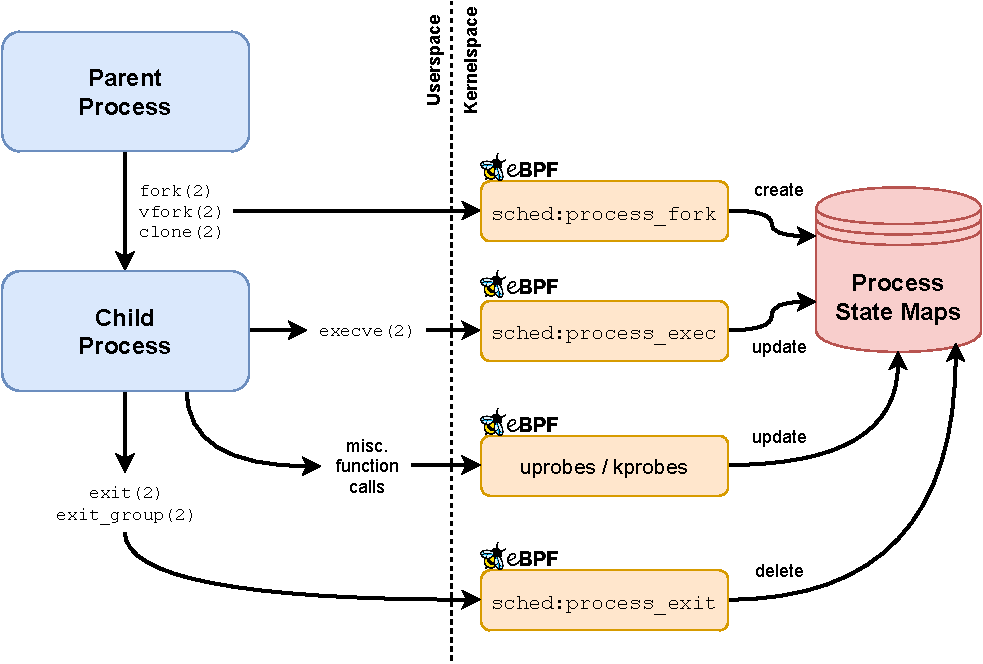
\includegraphics[width=0.8\linewidth]{figs/bpfbox/process-lifecycle.pdf}
  \caption[The various mechanisms that \bpfbox{} uses to manage process state]{
    The various mechanisms that \bpfbox{} uses to manage process state.
    Probes marked \texttt{sched:*} are tracepoints instrumenting scheduler events
    in the kernel. Uprobes and kprobes instrument userspace
    and kernelspace function calls respectively.
  }%
  \label{fig:bpfbox-process-lifecycle}
\end{figure}

%% \begin{lstlisting}[language=c, caption={The data structure stored in the \textit{process states} hashmap,
%% which \bpfbox{} uses to track the state of running tasks. The map is keyed by
%% thread ID.}, label={lst:process-state}]
%% struct bpfbox_process_t {
%%     /* Key of the profile associated with
%%      * this process. */
%%     u64 profile_key;
%%     /* A 64-bit vector representing
%%      * the current state of the process. */
%%     u64 state;
%% };
%% \end{lstlisting}

Instrumenting a tracepoint on \texttt{sched:process\_fork} allows \bpfbox{} to
detect when a new task is created via the \texttt{fork(2)}, \texttt{vfork(2)}, or
\texttt{clone(2)} system calls. This tracepoint creates an entry in the \textit{process
states} hashmap and initializes it according to the state of the parent process; if the
parent process is associated with a \bpfbox{} profile, its key is copied to the child
until such time as the child makes an \texttt{execve(2)} call.

The \texttt{sched:process\_exec} tracepoint is triggered whenever a task calls
\texttt{execve} to load a new program.  \bpfbox{} uses this tracepoint to manage the
association of \textit{policy keys} to a particular \textit{process state}.  \bpfbox{}
policy may optionally specify whether a transition from one profile to another may occur
in a given call to \texttt{execve}; this transition is disallowed by default.

Finally, the \texttt{sched:process\_exit} tracepoint allows \bpfbox{} to detect when
a task exits. This tracepoint deletes the corresponding entry in the \textit{process
states} map.

\subsection{Context-Aware Policy}
\label{ss:bpfbox-context-aware}

If the policy for a given executable defines specific function call contexts for
particular rules, \bpfbox{} instruments these function calls using uprobes (for userspace
functions) and kprobes (for kernelspace functions). Each instrumented function call is
associated with a unique bit in the process' \textit{state} bitmask.  A probe is triggered
on entry that causes \bpfbox{} to flip the corresponding bit to a \texttt{1}, and again on
return, flipping the corresponding bit back to a \texttt{0}.
\Cref{fig:bpfbox-function-calls} depicts how \bpfbox{} instruments userspace and
kernelspace function calls for policy enforcement.

\begin{figure}[p]
  \centering
  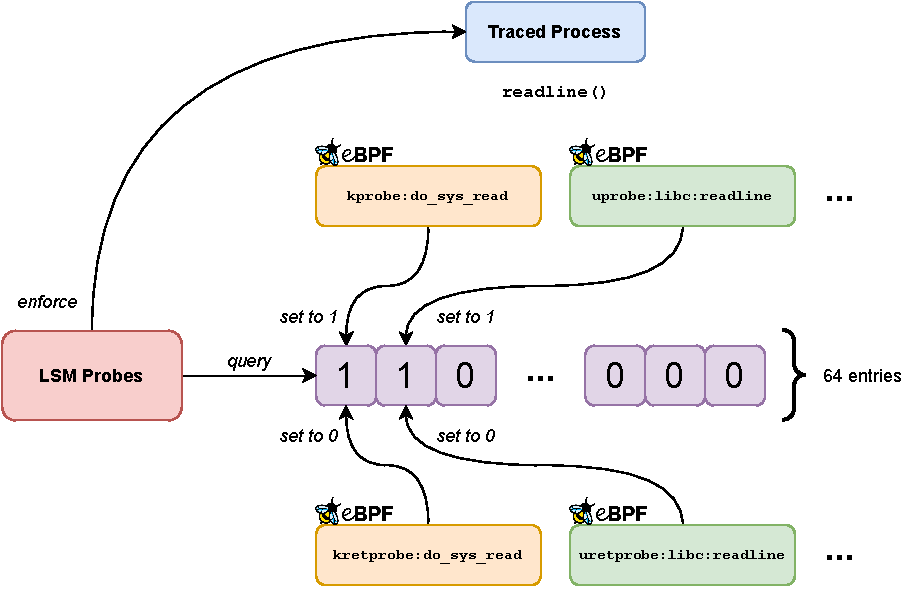
\includegraphics[width=1\linewidth]{figs/bpfbox/function-calls.pdf}
  \caption[How \bpfbox{} tracks function calls]{
    How \bpfbox{} uses kprobes and uprobes to track function calls.  If a policy
    identifies that a rule should apply within the context of a certain function call,
    \bpfbox{} instruments a probe on function entry and return. These probes flip the
    corresponding bit in the process' state vector, indicating to policy enforcement
    probes whether or not the process is in the middle of making the function call.
  }%
  \label{fig:bpfbox-function-calls}
\end{figure}

This approach is subject to a few inherent limitations.  Firstly, compile-time
optimizations such as function in-lining can invalidate the probe by removing the
corresponding symbol in the target object file. Secondly, a recursive call that is not
tail-optimized will break enforcement by prematurely signalling to \bpfbox{} that
a process has exited a given function context.  The first limitation may be trivially
worked around by hinting to the compiler that a given function should not be in-lined;
although this sacrifices some application transparency and incurs a slight performance
penalty, the potential security benefits from such a fine-grained policy are arguably
worth the trade-off.  The second limitation \textit{could} be worked around by maintaining
a reference counter for each function call rather than a flat vector. \bpfbox{} currently
does not do this, since it would incur a larger memory overhead for each active process,
but it would be possible to extend a future version of \bpfbox{} with this workaround. In
case working around these limitations is impractical, the policy author would simply fall
back to specifying ordinary rules rather than context-specific ones.



\subsection{Collecting and Logging Audit Data}%
\label{ss:bpfbox-audit}

When an operation is denied or matches with an audit rule, \bpfbox{} submits an event to
userspace for logging. To accomplish this, we leverage the new ringbuf map type added in
Linux 5.8. The \gls{ebpf} ringbuf map implements an efficient ring buffer that is shared
across all \glspl{cpu}. This new map type comes with a number of optimizations for fast
reads and writes and in-order guarantees for asynchronous events across multiple
\glspl{cpu}, allowing per-event data to be efficiently shared with userspace in near
real-time.

In userspace, the \bpfbox{} daemon uses \texttt{mmap(2)} to map the corresponding memory
region and polls for new data at regular intervals. As events are consumed in userspace
they are removed from the ring buffer to make room for new events.  Since the ringbuf map
provides strong order guarantees and high performance under contention, we can ensure that
\bpfbox{} always provides highly reliable and performant per-event auditing.



\section{\bpfbox{} Policy Language}%
\label{s:bpfbox-policies}

\bpfbox{} policies are a series of rules and accompanying decorators. A decorator may
annotate either individual rules or blocks of rules denoted by braces and is used to
specify additional context or policy actions. The first line in a \bpfbox{} policy is
always a special \enquote{profile decorator}, written as
\lstinline[language=bpfbox]{#![profile "/path/to/exe"]}, which marks the executable to
which the policy should be associated.  Other than the profile decorator, all others take
the form of \lstinline[language=bpfbox]|#[decorator] { rule() }|. Multiple decorators may
be specified before a set of rules, meaning that all decorators apply to each rule.

Profile assignment occurs when a process makes an \texttt{execve(2)} call that results in
loading the specified executable.  Once a process has been assigned a profile, this
profile cannot change again, unless an \texttt{execve(2)} occurs which has been explicitly
marked with the \lstinline[language=bpfbox]{#[transition]} decorator. This ensures that
policy transitions only occur when expected and prevents malicious \texttt{execve(2)}
calls from changing \bpfbox{}'s treatment of a process.

The sections that follow describe the rule categories supported by \bpfbox{}
(\Crefrange{ss:bpfbox-filesystem-rules}{ss:bpfbox-ptrace-rules}) and the decorators that
may optionally be used to augment them (\Crefrange{ss:bpfbox-allow}{ss:bpfbox-kfunc}).
\Cref{lst:bpfbox-policy-example} depicts a simple example \bpfbox{} policy.

\begin{lstlisting}[language=bpfbox, gobble=4,
  caption={[An example \bpfbox{} policy]
    An example \bpfbox{} policy for a simple remote login program. This example offers
    a fairly complete idea of the \bpfbox{} policy language's various features.
  },
  label={lst:bpfbox-policy-example}, float]
    /* This policy applies to the /usr/bin/mylogin
     * executable */
    #![profile "/usr/bin/mylogin"]

    /* Taint process state upon binding to
     * any IPv4/IPv6 network socket */
    #[taint] {
      net(inet,  bind)
      net(inet6, bind)
    }

    /* Allow network connections/operations */
    #[allow] {
      net(inet,  accept|listen|send|recv)
      net(inet6, accept|listen|send|recv)
    }

    /* Allow the check_login function to read
     * /etc/passwd and /etc/shadow */
    #[func "check_login"] {
      fs("/etc/passwd", read)
      fs("/etc/shadow", read)
    }

    /* Allow the add_user function to read
     * and append to /etc/passwd, but log such
     * events to the audit logs */
    #[func "add_user"]
    #[audit] {
      fs("/etc/passwd", read|append)
    }

    /* Read and append to any immediate child
     * of the /var/log/mylogin/ directory */
    fs("/var/log/mylogin/*", read|append)

    /* Allow the execution of /bin/bash, transitioning
     * profiles to bash's profile after the execve(2)
     * and untainting the process */
    #[transition]
    #[untaint] {
      fs("/bin/bash", read|exec)
    }
\end{lstlisting}



\subsection{Filesystem Rules}%
\label{ss:bpfbox-filesystem-rules}

Filesystem rules in \bpfbox{} govern what operations a process may perform on filesystem
objects such as files and directories. They are written as
\lstinline[language=bpfbox]{fs("pathname", access)} where
\lstinline[language=bpfbox]{"pathname"} is a string containing the pathname of the file
and \lstinline[language=bpfbox]{access} is a list of one or more file access permissions
joined by the vertical bar symbol.  For instance, to represent read and
append permissions on \texttt{/var/log/my\_log}, the corresponding \bpfbox{} rule would be
\lstinline[language=bpfbox]{fs("/var/log/my_log", read|append)}.  In total, \bpfbox{}
supports nine distinct filesystem access flags as shown in \Cref{tab:fs-access}.

\begin{table}[htpb]
    \centering
    \caption{The filesystem access flags supported in \bpfbox{}.}
    \label{tab:fs-access}
    \begin{tabular}{lp{0.7\linewidth}}
    \toprule
    Flag & Meaning \\
    \midrule
    \texttt{read}    & The subject may read the object. \\
    \texttt{write}   & The subject may write to the object. \\
    \texttt{append}  & The subject may append to the object. \\
    \texttt{exec}    & The subject may execute the object. \\
    \texttt{setattr} & The subject may change the object's filesystem attributes. \\
    \texttt{getattr} & The subject may read the object's filesystem attributes. \\
    \texttt{rm}      & The subject may remove the object's inode. \\
    \texttt{link}    & The subject may create a link to the object's inode. \\
    \texttt{ioctl}   & The subject may perform an ioctl call on the object. \\
    \bottomrule
    \end{tabular}
\end{table}

\bpfbox{} supports a limited globbing syntax when defining pathnames, allowing multiple
rules matching similar files to be combined into one.  Although filesystem rules are
specified using pathnames, \bpfbox{} internally uses inode and device numbers rather than
the pathnames themselves. When loading policies, \bpfbox{} automatically resolves the
provided pathnames into their respective inode-device number pairs. This information is
then used to look up the correct policy whenever a sandboxed application attempts to
access an inode.  Since \bpfbox{} does not check the pathnames themselves when referring
to files, it is able to defeat \glsentryfull{toctou} attacks, where an
attacker quickly swaps out one file with a link to another in an attempt to circumvent
access control restrictions in a privileged (most often setuid)
binary~\cite{bishop1996_checking}.  In such a situation, \bpfbox{} would simply see
a different inode and deny access.

In addition to regular filesystem rules, \bpfbox{} provides a special rule type for
\texttt{/proc/pid} entries in the \texttt{procfs} virtual filesystem. \texttt{procfs}
rules, written as \lstinline[language=bpfbox]{proc("exe", access)} where
\lstinline[language=bpfbox]{"exe"} is a string containing the pathname of another
executable and \lstinline[language=bpfbox]{access} is the desired access. For example,
read-only access to the \texttt{procfs} entries of executables running
\texttt{/usr/bin/ls} may be specified with \lstinline[language=bpfbox]{proc("/usr/bin/ls", read)}.
Access to any \texttt{procfs} entry may be specified using the special keyword
\lstinline[language=bpfbox]{any}.



\subsection{Network Rules}%
\label{ss:bpfbox-network-rules}

\bpfbox{} implements networking policy at the socket level, covering both Internet sockets
as well as Unix domain sockets. Networking rules are specified using
\lstinline[language=bpfbox]{net(protocol, access)}, where
\lstinline[language=bpfbox]{protocol} is a networking protocol like \texttt{inet},
\texttt{inet6}, or \texttt{unix} and \lstinline[language=bpfbox]{access} is a list of
socket operations (\Cref{tab:net-access}) separated by vertical bars. For example, a rule
targeting \texttt{bind}, \texttt{accept}, and \texttt{connect} operations on an
\texttt{inet6} socket would look like \lstinline[language=bpfbox]{net(inet6, bind|connect|accept)},
while a rule targeting \texttt{create} operations on a \texttt{unix} socket would look
like \lstinline[language=bpfbox]{net(unix, create)}.

\begin{table}[htpb]
    \centering
    \caption{The socket operation flags supported in \bpfbox{}.}
    \label{tab:net-access}
    \begin{tabular}{lp{0.7\linewidth}}
    \toprule
    Flag & Meaning \\
    \midrule
    \texttt{connect}  & Subject may connect a socket to a remote address. \\
    \texttt{bind}     & Subject may bind a socket to a local address. \\
    \texttt{accept}   & Subject may accept an incoming socket connection. \\
    \texttt{listen}   & Subject may listen for incoming socket connections. \\
    \texttt{send}     & Subject may send messages over a socket. \\
    \texttt{recv}     & Subject may receive messages over a socket. \\
    \texttt{create}   & Subject may create new sockets. \\
    \texttt{shutdown} & Subject may shut down a socket connection. \\
    \bottomrule
    \end{tabular}
\end{table}



\subsection{Signal Rules}%
\label{ss:bpfbox-signal-rules}

Specifying signal behaviour in \bpfbox{} is done using the
\lstinline[language=bpfbox]{signal("exe", access)} where
\lstinline[language=bpfbox]{"exe"} is the pathname of another executable and
\lstinline[language=bpfbox]{access} is a list of signals allowed to be sent, separated by
vertical bars. Normally, only processes running the executable
\lstinline[language=bpfbox]{"exe"} are allowed to be signalled, but the special keyword
\lstinline[language=bpfbox]{any} may be used instead to specify the ability to signal
\textit{any} process on the system. Two additional keywords,
\lstinline[language=bpfbox]{parent} and \lstinline[language=bpfbox]{child}, allow parent
and child processes to be signalled instead.  The \lstinline[language=bpfbox]{access}
argument supports any Linux signal, in addition to a few helper keywords that can be used
to specify broad categories, such as \lstinline[language=bpfbox]{fatal} for fatal signals
and \lstinline[language=bpfbox]{nohandle} for signals that cannot be handled.  For
example, to specify the ability to send fatal signals to any process running
\texttt{/usr/bin/ls}, the corresponding \bpfbox{} rule would be
\lstinline[language=bpfbox]{signal("/usr/bin/ls", fatal)}.  To narrow permissions such
that only \texttt{SIGTERM} and \texttt{SIGINT} are allowed,
\lstinline[language=bpfbox]{signal("/usr/bin/ls", sigterm|sigint)} could be used instead.



\subsection{Ptrace Rules}%
\label{ss:bpfbox-ptrace-rules}

Just like with signals, \texttt{ptrace} access is specified as
\lstinline[language=bpfbox]{ptrace("exe", access)}, where
\lstinline[language=bpfbox]{access} is a list of allowed \texttt{ptrace} modes separated
by vertical bars. The \lstinline[language=bpfbox]{child} keyword is also available for
\texttt{ptrace} rules to allow tracing of any child process, regardless of the child's
current profile. For instance, a rule that allows a process to read and attach to a child
process would be written as \lstinline[language=bpfbox]{ptrace(child, read|attach)}, while
a rule that allows only read access to processes running \texttt{/usr/bin/ls} would be
written as \lstinline[language=bpfbox]{ptrace("/usr/bin/ls", read)}.  Note that currently
\texttt{ptrace} rules do not override other \texttt{ptrace} restrictions, such as those
imposed by Yama~\cite{yama}.



\subsection{Allow, Taint, and Audit Decorators}%
\label{ss:bpfbox-allow}

\bpfbox{} supports three distinct decorators for defining \textit{actions} that should be
taken when a given access matches a rule. The \lstinline[language=bpfbox]{#[allow]}
decorator causes \bpfbox{} to allow the access; however, it is not typically necessary to
explicitly specify this as undecorated rules are assumed to be allowed by default.
Regardless, it may be desirable to decorate such rules with
\lstinline[language=bpfbox]{#[allow]} to improve the clarity of the policy.
\lstinline[language=bpfbox]{#[taint]} is used to mark a rule as a \textit{taint rule},
which causes the process to enter a tainted state when matched. These rules can be thought
of as gateways into the rest of the policy.  Once a process is tainted, this cannot be
reversed unless it makes an \texttt{execve(2)} call explicitly marked with
\lstinline[language=bpfbox]{#[untaint]}.  Finally, \lstinline[language=bpfbox]{#[audit]}
may be combined with \lstinline[language=bpfbox]{#[allow]} to cause \bpfbox{} to log the
matching operation to its audit logs. This can be useful for marking rare behaviour that
should be investigated or for determining how often a given rule is matched in practice.



\subsection{Func and Kfunc Decorators}%
\label{ss:bpfbox-kfunc}

One of the key features of \bpfbox{} is the ability to specify specific application-level
and kernel-level context for rules. In the policy language, this is done by decorating
rules with the \lstinline[language=bpfbox]{#[func "fn_name" ("filename")]} and
\lstinline[language=bpfbox]{#[kfunc "fn_name"]} decorators for userspace and kernelspace
instrumentation respectively. Here, \lstinline[language=bpfbox]{"fn_name"} refers to the
name of the function to be instrumented and \lstinline[language=bpfbox]{"filename"} refers
to the filename where the function symbol should be looked up --- this parameter is
optional and allows for the instrumentation of shared libraries.  These decorators provide
powerful tools for defining extremely fine-grained, sub-application level policy. For
instance, to declare that read access to the file \texttt{/etc/shadow} should only occur
during a call to the function \texttt{check\_password()}, the corresponding \bpfbox{} rule
would look like:
\begin{lstlisting}[language=bpfbox]
#[func "check_password"]
fs("/etc/shadow", read)
\end{lstlisting}
A process that is sandboxed using this policy would be unable to access
\texttt{/etc/shadow} except within a call to the specified function.



\section{Limitations and the Transition Toward \bpfcontain{}}%
\label{s:bpfbox-bpfcontain}

While \bpfbox{} certainly offers a new perspective on confinement and improves the status
quo, the extent to which it achieves the design goals outlined in \Cref{s:cp-design} is
arguably hampered by a few inherent limitations. We address these limitations in its
successor, \bpfcontain{}, the design of which is outlined in the next chapter. Before we
examine \bpfcontain{} in full, we first address the fundamental limitations of \bpfbox{}
as a confinement mechanism and offers some insights into how \bpfcontain{} addresses them.
\begin{enumerate}
  \item \textbf{Dependency Overhead and Runtime Overhead.}
    Due to its userspace implementation using bcc, \bpfbox{} has a high dependency
    overhead. This overhead is the combined result of a number of requirements imposed on
    the host system by the bcc toolchain. On the userspace side, bcc depends on Python as
    well as the entire LLVM toolchain for program compilation. Both of these are rather
    hefty requirements on their own. Python requires an entire language runtime, and
    a full LLVM toolchain can introduce gigabytes of additional code.

    Furthermore, Python and bcc incur significant runtime overhead. Python is an
    interpreted language with a much heavier runtime than compiled systems languages like
    C or Rust.  This runtime incurs additional performance disadvantages due to safety
    features like the global object lock, which impede concurrency. Since bcc compiles
    \gls{ebpf} programs at runtime, we incur additional compilation overhead for each
    program, sometimes resulting in significant startup delays depending on the complexity
    of the application. This runtime compilation also necessitates the availability of
    kernel headers as a compilation dependency in the target environment, adding further
    storage overhead.

    \bpfcontain{} solves these dependency and runtime overhead issues by leveraging Rust
    and libbpf \gls{core}~\cite{nakryiko2020_core} rather than Python and bcc.  Unlike
    bcc, libbpf \gls{core} enables \gls{bpf} programs to be compiled once and run
    anywhere, thanks to \gls{btf} information provided by the kernel and load-time symbol
    relocation. Program bytecode can then be embedded directly into the compiled object
    file, meaning the single pre-compiled \bpfcontain{} binary can be deployed on any
    target kernel that meets a minimal set of requirements. As a side effect,
    \bpfcontain{} requires neither a full LLVM toolchain nor kernel headers to be
    available in the target deployment, significantly reducing the dependency overhead.

    Moreover, implementing the \bpfcontain{} daemon in Rust allows \bpfcontain{} to take
    advantage of a myriad of benefits offered by the Rust language. In particular, Rust
    enables \bpfcontain{}'s userspace components to be safe, secure, and fast. Thread- and
    memory-safety guarantees provided by Rust ownership model eliminate many common
    security bugs including memory corruption vulnerabilities and race conditions between
    threads. These safety guarantees provide critical security advantages, particularly
    given the fact that the \bpfcontain{} daemon is a long-running, privileged
    process\,---\,a ripe target for attacker exploitation. Thanks to an emphasis on speed
    and zero-cost abstractions, Rust can provide these benefits at virtually zero
    overhead, in line with traditional systems programming languages like C and
    significantly better than languages with a bulky runtime such as Python.

  \item \textbf{Lack of Container Semantics.}
    Although \bpfbox{} exposes a light-weight policy language with high-level semantics to
    the user, it fails to consider container semantics, as outlined in design goal
    \ref{i:dg-suitability} in \Cref{s:cp-design}. While this marks an improvement over
    existing confinement solutions by offering a terse yet fine-grained and expressive
    policy language, it fails to fully address the container-specific use case; in other
    words, \bpfbox{} is more suitable to generic, ad-hoc application sandboxing than to
    container-specific applications. In improving the way the \bpfbox{} model handles
    containers, we can simultaneously simplify policies and improve security by defining
    a clear protection boundary around a container.

    \bpfcontain{} rectifies this gap by incorporating container semantics into the design
    of both its policy language and enforcement engine. This includes properties such as
    namespace and container membership, defining an implicit boundary around the container
    and related resources, similar in spirit to FreeBSD Jails~\cite{kamp2000_jails}. In
    this way, \bpfcontain{} policies can grant access to objects that exist within the
    container and revoke access to objects that exist outside the container. Policies then
    focus on defining exceptions to this boundary, exposing fine-grained interfaces into
    the container and locking down the rest by default.

  \item \textbf{Policy Language Simplification.}
    In addition to adding container semantics, other aspects of the \bpfbox{} policy
    language can also be improved and simplified. For instance, \bpfbox{} implements
    policy in a domain-specific policy language, designed specifically with \bpfbox{}'s
    enforcement engine in mind. While effective, this approach is tightly-coupled with
    policy enforcement and introduces additional cognitive overhead when making extensions
    to or modifying the policy language design. Furthermore, learning the syntax of
    a custom policy language can introduce an additional barrier-to-entry for new policy
    authors, to the detriment of \bpfbox{}'s original goal of making policy authorship
    available to end-users.

    To rectify these issues in the policy language design, \bpfcontain{} eschews the
    original policy language and instead reaches for a more modular approach.  Rather than
    defining an entire new policy language, \bpfcontain{} instead defines a policy
    language \textit{schema}. This schema can then be encoded in any number of available
    data serialization formats, including YAML~\todo{CITE}, JSON~\todo{CITE},
    TOML~\todo{CITE} and others. The end result is that the user is able to choose
    whichever policy encoding they are most comfortable with, using serialization
    languages that are both commonly available and that have stood the test of time across
    a variety of production use cases. Another implicit advantage of this approach is that
    it enables the future integration of \bpfcontain{} policy into existing container
    specification schemas, such as the \gls{oci} specification, which is encoded in
    JSON\@.
\end{enumerate}



\section{Summary}%
\label{s:bpfbox-summary}

This chapter has presented the design and implementation of \bpfbox{}, a prototype process
confinement mechanism leveraging \gls{ebpf} for dynamically loadable policies that balance
simplicity and flexibility. In particular, we outline \bpfbox{}'s architecture, the
implementation details of its \gls{ebpf}-based policy enforcement mechanism, and the
design of its custom policy language. Through a combination of \gls{ebpf}-based
enforcement and a light-weight yet fine-grained policy language, \bpfbox{} represents
a step towards the container-specific design outlined in \Cref{s:cp-design}. However, we
acknowledge some fundamental limitations with \bpfbox{}'s design, including dependency
overhead, lack of container semantics, and room for further simplification of its policy
language. In the next chapter, we outline \bpfcontain{}, an iteration of \bpfbox{} that
addresses these concerns.


\chapter{\bpfcontain: Extending \bpfbox{} to Model Containers}%
\label{c:bpfcontain}
In this chapter, we present \bpfcontain{}, an iteration on the original \bpfbox{} system
presented in \Cref{c:bpfbox}. \bpfcontain{} is a superset of \bpfbox. In particular, it is
a streamlined re-implementation that focuses on container-specific confinement policy, low
dependency overhead, and maximizing adoptability. Portions of this chapter are taken from
an upcoming paper, co-authored with David Barrera and Anil Somayaji, and planned for
submission at USENIX Security 2022. A draft of this paper is currently
available~\cite{findlay2021_bpfcontain}, although significant portions of this chapter
differ from the publicly available archive due to subsequent updates to \bpfcontain{}.



\section{\bpfbox{}'s Limitations and the Transition Toward \bpfcontain{}}%
\label{s:bpfcontain-bpfbox-limitations}

The previous chapter presented \bpfbox{}, a prototype process confinement mechanism and
precursor to \bpfcontain{}. While \bpfbox{} certainly offers a new perspective on
confinement and improves the status quo, the extent to which it achieves the design goals
outlined in \Cref{s:cp-design} of \Cref{c:confinement-problem} is arguably hampered by
a few inherent limitations. We enumerate and describe these limitations as follows.  The
goal is to examine these limitations as an early motivating factor for the development of
\bpfcontain{}, which will inform later comparisons between these two systems
(c.f.~\Cref{s:bpfcontain-improvements}).

\begin{enumerate}
  \item \textbf{Dependency Overhead and Runtime Overhead.}
    Due to its userspace implementation using bcc, \bpfbox{} has a high dependency
    overhead. This overhead is the combined result of a number of requirements imposed on
    the host system by the bcc toolchain. On the userspace side, bcc depends on Python as
    well as the entire LLVM toolchain for program compilation. Both of these are rather
    hefty requirements on their own. Python requires an entire language runtime, and
    a full LLVM toolchain can introduce gigabytes of additional code.

    Furthermore, Python and bcc incur significant runtime overhead. Python is an
    interpreted language with a much heavier runtime than compiled systems languages like
    C or Rust.  This runtime incurs additional performance disadvantages due to safety
    features like the global object lock, which impede concurrency. Since bcc compiles
    \gls{ebpf} programs at runtime, we incur additional compilation overhead for each
    program, sometimes resulting in significant startup delays depending on the complexity
    of the application. This runtime compilation also necessitates the availability of
    kernel headers as a compilation dependency in the target environment, adding further
    storage overhead.

  \item \textbf{Lack of Container Semantics.}
    Although \bpfbox{} exposes a light-weight policy language with high-level semantics to
    the user, it fails to consider container semantics, as outlined in design goal
    \ref{i:dg-suitability} in \Cref{s:cp-design}. While this marks an improvement over
    existing confinement solutions by offering a terse yet fine-grained and expressive
    policy language, it fails to fully address the container-specific use case; in other
    words, \bpfbox{} is more suitable to generic, ad-hoc application sandboxing than to
    container-specific applications. In improving how the \bpfbox{} model handles
    containers, we can simultaneously simplify policies and improve security by defining
    a clear protection boundary around a container.

  \item \textbf{Policy Language Simplification.}
    In addition to adding container semantics, other aspects of the \bpfbox{} policy
    language can also be improved and simplified. For instance, \bpfbox{} implements
    policy in a domain-specific policy language, designed specifically with \bpfbox{}'s
    enforcement engine in mind. While effective, this approach is tightly-coupled with
    policy enforcement and introduces additional cognitive overhead when making extensions
    to or modifying the policy language design. Furthermore, learning the syntax of
    a custom policy language can introduce an additional barrier-to-entry for new policy
    authors, to the detriment of \bpfbox{}'s original goal of making policy authorship
    available to end-users.
\end{enumerate}

\subsection{Motivating \bpfcontain{}}

The key insight behind \bpfcontain{} is that \bpfbox{} approached the confinement problem
(c.f.~\Cref{c:confinement-problem}) from a \textit{per-process} perspective. When dealing
with containers, we should instead approach the confinement problem from
a \textit{per-process-group} perspective. That is, we expand the unit of confinement from
an individual process to a collection of related processes. Specifically, our goal is to
define a clear boundary between the container and the outside world, while minimizing the
friction between two subjects that operate within this boundary.

Implementing confinement in this way requires some fundamental changes to both the
underlying policy language and policy enforcement mechanism. Specifically, we alter the
policy language to work with higher level semantics that support container-level
confinement. Moreover, \bpfcontain{}'s enforcement engine employs a more nuanced default
policy that considers the relationship between processes and resources that exist within
the context of a container. These changes from a policy and enforcement perspective enable
\bpfcontain{} to enforce simple container-level policies while reusing the initial ideas
from \bpfbox{}: namely, dynamic, light-weight enforcement based on \gls{ebpf}.

While implementing \bpfcontain{}, opportunities arose to improve how it handles
dependencies and manages the lifecycle of its \gls{bpf} programs and maps. Specifically,
we architect \bpfcontain{} based on Rust, libbpf-rs~\cite{libbpf-rs}, and \gls{bpf}
\gls{core}~\cite{nakryiko2020_core}. These changes totally eliminate the runtime overhead
introduced by \gls{bpf} program compilation and the dependency overhead from LLVM and
kernel headers. Further, \gls{core} enables \bpfcontain{} to work seamlessly across
multiple kernel versions and configurations. These changes improve the adoptability of
\bpfcontain{}, particularly in containerized environments, wherein heavy-weight
dependencies can critically impact deployments.

\todo{Maybe add a short paragraph here to lead into the next sections?}

\section{\bpfcontain{} Overview}%
\label{s:bpfcontain-overview}

\bpfcontain{} is a container security daemon for Linux that focuses on simple, high-level
confinement policies for container deployments. Although it is expressly designed to work
with container semantics in mind, \bpfcontain{} implements a superset of \bpfbox{}'s
capabilities (c.f.~\Cref{c:bpfbox}) and works for confining ordinary applications as well
as containers. To achieve confinement, \bpfcontain{} leverages \gls{ebpf} programs
attached to \gls{lsm} hooks in the kernel for security enforcement.

As a container-specific confinement solution, \bpfcontain{} has a number of important
design goals, some of which are shared with \bpfbox{}. First, we seek to design a simple
yet flexible policy language that supports ad-hoc confinement use cases, enabling an
end-user to write a custom confinement policy to suit their needs. We extend this goal by
seeking to make the policy language and enforcement engine \textit{container-specific}.
This means that \bpfcontain{} policies should conform to container semantics and work in
tandem with container virtualization primitives to improve policy enforcement and further
simplify the underlying policies. Finally, \bpfcontain{} should be readily adoptable in
production use cases and should be useful for confining existing container workloads.

At the surface level, \bpfcontain{}'s architecture is similar to that of \bpfbox{}, albeit
with significant differences in implementation and design details. In a nutshell,
\bpfcontain{} is implemented as a privileged userspace daemon that loads \gls{ebpf}
programs and maps into the kernel, which then enforce policy.
\Cref{ss:bpfcontain-enforcement-overview} provides a high-level overview of how
\bpfcontain{} enforces policy, whereas \Cref{s:bpfcontain-implementation} covers
\bpfcontain{}'s architecture and implementation details in full.

\subsection{Policy Enforcement at a High Level}%
\label{ss:bpfcontain-enforcement-overview}

\bpfcontain{} enforces confinement policy using \gls{ebpf} programs attached to \gls{lsm}
hooks in the kernel. Like \bpfbox{}, \bpfcontain{} leverages the
\gls{krsi}~\cite{singh2019_krsi} \gls{lsm} programs introduced in Linux 5.8 for this
purpose. Unlike \bpfbox{}, \bpfcontain{} generates \gls{bpf} bytecode at
\textit{compile-time} rather than at runtime. The bytecode is then embedded directly in
\bpfcontain{}'s binary object file, where it can subsequently be loaded into the kernel at
runtime.

To confine a container, a user authors a high-level confinement policy that specifies
which operating system interfaces and resources should be exposed to the container.
Thanks to a modular approach to encoding and decoding policies, \bpfcontain{} policies may
be written in a number of user-facing data serialization languages, including YAML, TOML,
and JSON. (For the rest of this thesis, we assume the YAML format for simplicity.) At
a minimum, \bpfcontain{} policies include a policy name, along with a few tunable
parameters.  From there, the user may specify zero or more policy rules over three
distinct categories: allow, deny, and taint. We cover \bpfcontain{} policy in more detail
in \Cref{s:bpfcontain-policy}.

\begin{figure}[htpb]
  \centering
  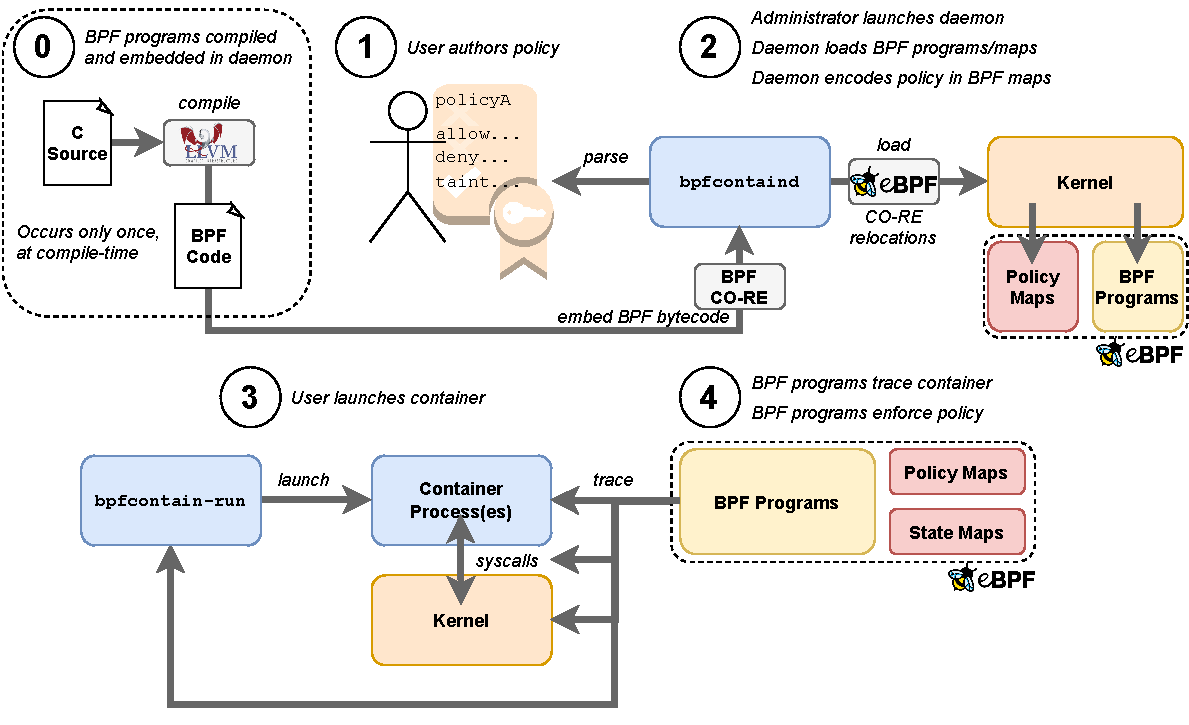
\includegraphics[width=1\linewidth]{figs/bpfcontain/overview.pdf}
  \caption[A high-level overview of how \bpfcontain{} confines applications]{
    A high-level overview of how \bpfcontain{} confines applications.  At compile-time,
    the object code for \bpfcontain{}'s \gls{bpf} programs is embedded directly into the
    resulting binary. To confine a container, the user first authors a high-level policy
    in their chosen data serialization language. The daemon parses this policy and loads
    it into the kernel by encoding it into \gls{ebpf} maps. The user then launches the
    container using the \texttt{bpfcontain-run} wrapper, at which point \bpfcontain{}
    begins tracing it and enforcing policy. Note the subtle differences between this
    figure and \Cref{fig:bpfbox-policy-overview} in \Cref{c:bpfbox}.
  }%
  \label{fig:bpfcontain-overview}
\end{figure}

The \bpfcontain{} daemon runs as a privileged process, parsing and loading user policy by
encoding it into a series of \gls{bpf} maps. The user then launches their container using
an unprivileged wrapper program, \texttt{bpfcontain-run}. The sole task of this wrapper
application is to invoke a stub function which does nothing more than pass the desired
policy ID as an argument. \bpfcontain{} traces this function call and uses it to confine
the container with the correct policy. Unlike \bpfbox{}, this technique enables the user
to associate any container with any policy, rather than a fixed one-to-one mapping.

At runtime, \bpfcontain{}'s \gls{bpf} programs trace the behaviour of processes running
under the container and confine it according to a mixture of default policy and policy
rules specified by the user. Like \bpfbox{}, enforcement is accomplished primarily through
\gls{bpf} programs attached to \gls{lsm} hooks in the kernel. The precise implementation
details of these programs vary significantly, and are covered in detail in
\Cref{s:bpfcontain-implementation}. \Cref{fig:bpfcontain-overview} illustrates
a high-level overview of the policy enforcement process described here.



\section{\bpfcontain{} Implementation}%
\label{s:bpfcontain-implementation}

This section presents the implementation details and architecture of \bpfcontain{}'s
policy enforcement mechanism. Specifically, we provide an initial overview of
\bpfcontain{}'s userspace and kernelspace components, then examine how \bpfcontain{}
enforces policy in the kernel using \gls{ebpf}. Whereas this section focuses specifically
on policy enforcement, \Cref{s:bpfcontain-policy} outlines and documents the details of
\bpfcontain{}'s policy language.

\subsection{Architectural Overview}%
\label{ss:bpfcontain-architecture}

Like \bpfbox{}, \bpfcontain{} is implemented as privileged daemon that runs in userspace
and loads \gls{ebpf} code into the kernel for policy enforcement. However, the precise
architecture and implementation details of this daemon are quite different. In particular,
the daemon is implemented in Rust and leverages the libbpf-rs crate\footnote{A crate is
a Rust package that can be added as a dependency to a project. For the purposes of this
thesis, we can consider the terms \enquote{crate} and \enquote{library} to be
equivalent.}~\cite{libbpf-rs} to load its \gls{ebpf} programs and maps into the kernel.
This results in a number of advantages, which we discuss in more detail in the following
section.

\bpfcontain{}'s kernelspace components are implemented in \gls{ebpf}. \gls{ebpf} programs
trace container lifecycle and enforce policy, while \gls{ebpf} maps store policy and pass
intermediary state between program invocations. This architecture is similar in spirit to
the design of \bpfbox{}, but with a few fundamental differences. Firstly, rather than
using the LLVM toolchain to compile programs at runtime, \bpfcontain{} pre-compiles and
embeds the \gls{bpf} object code into its binary object file. Using \gls{bpf}
\gls{core}~\cite{nakryiko2020_core}, these programs can then be dynamically loaded into
any supported kernel, regardless of the underlying configuration or architectural details.

\bpfcontain{} leverages several \gls{bpf} program and map types to implement container
tracing and confinement. While many of the major program types are shared with \bpfbox{},
there are a few distinct differences (c.f.~\Cref{ss:bpfbox-architecture} of
\Cref{c:bpfbox}). We enumerate these differences as follows. Map types are outlined in
\textbf{\green{green}} and program types are outlined in \textbf{\purple{purple}}.
\begin{itemize}
  \item \bpfcontain{} replaces many of \bpfbox{}'s \textbf{\green{Hash Maps}},
  particularly those used to track process state, with equivalent \textbf{\green{Local
  Storage Maps}}. Local storage is a new \gls{ebpf} map type supported in the latest
  kernels (Linux 5.11 and onwards). Local storage maps tether the underlying value to
  a kernel data structure, such as a task or inode, used as a key into the map. The result
  is a dynamically-allocated and garbage-collected per-structure storage blob.
  \bpfcontain{} leverages these for more memory-efficient storage of per-task and
  per-inode state.

  \item \bpfcontain{} replaces the use of scheduler \textbf{\purple{Tracepoints}} with
  equivalent \textbf{\purple{\gls{lsm} Probes}} that expose the same information. This
  reduces potential overhead from multiple \gls{bpf} program invocations on the same code
  path, most notably over \texttt{fork(2)} and \texttt{clone(2)} family system calls.

  \item \bpfcontain{} uses \textbf{\purple{Fentry and Fexit}} probes in place of
  \textbf{\purple{Kprobes}}. These use a more efficient trampoline technique for program
  entry and use \gls{btf} information exposed by the kernel for direct memory access,
  making them far more efficient than kprobes.
\end{itemize}

Aside from the aforementioned differences, \bpfcontain{} uses the same \gls{bpf} program
and map types as \bpfbox{}. However, the underlying implementation details of each
\gls{bpf} program will be quite different from \bpfbox{}, as \bpfcontain{} is dealing with
container semantics, new policy rules, and more nuanced policy defaults. We examine the
most important implementation details in the subsections that follow.



\subsection{Policy Deserialization and Loading}%
\label{ss:bpfcontain-serde}

\bpfcontain{} implements policy deserialization using the Serde data serialization
crate~\todo{CITE} for Rust. Serde leverages Rust's powerful type system and procedural
macros to derive serialization and deserialization logic for vanilla Rust structs and
enums. Rust crates that consume Serde's \gls{api} can then use the automatically generated
facade for serialization and deserialization. This design enables a plug-and-play
relationship between a data schema, defined as a Rust data structure and any data
serialization language supported through the Rust crates ecosystem. \bpfcontain{} uses
Serde to automatically generate the accompanying deserialization logic for
a \texttt{Policy} struct and several \texttt{Rule} structs, one for each supported rule
type. \Cref{lst:bpfcontain-serde} depicts a simplified example of how this works.

\begin{lstlisting}[language=Rust, gobble=2, caption={[A simplified example of \bpfcontain{}'s policy deserialization logic]
  A simplified example of \bpfcontain{}'s policy deserialization logic. Policy rules are
  specified declaratively using Rust structs and the corresponding deserialization logic
  is automatically generated by the Serde crate, using a simple decorator macro.
},
label={lst:bpfcontain-serde}]
  use serde::Deserialize;

  /// The policy data structure
  #[derive(Deserialize)]
  pub struct Policy {
    name: String,
    /* Other policy metadata would go here... */
    allow: Vec<Rule>,
    deny: Vec<Rule>,
    taint: Vec<Rule>,
  }

  /// An enum encompassing all rule types
  #[derive(Deserialize)]
  pub enum Rule {
    FileRule(FileRule),
    /* Other rule types would go here... */
  }

  /// A "file access" rule
  #[derive(Deserialize)]
  pub struct FileRule {
    pathname: String,
    access: String,
  }

  /* Other rule types would go here... */
\end{lstlisting}

To enable the daemon to encode policy as an \gls{ebpf} map, each rule type implements the
\texttt{LoadableRule} trait. The daemon uses this logic to convert a policy rule into
a canonical format that can be represented in the kernel and thus used to enforce security
policy. Implementing this trait is as simple as writing a \texttt{load()} function that
makes a series of map updates to load the rule into the kernel; we leverage
libbpf-rs~\cite{libbpf-rs} for this purpose. When loading a policy into the kernel, the
daemon simply invokes this \texttt{load()} function for each policy rule.

Implementing policy deserialization and loading logic in this way has a number of
advantages. Since the policy schema is simply encoded declaratively in vanilla Rust, it is
easy for a developer (even a new contributor to \bpfcontain{}) to implement a new rule
type and add it to \bpfcontain{}. Adding a new rule type is as simple as defining a new
Rust data type to represent the rule and implementing the \texttt{LoadableRule} trait,
enabling the daemon to encode the rule as an \gls{ebpf} map. Due to Serde's modular
design, supporting a new serialization language for \bpfcontain{} policies is trivial; we
simply pull in the corresponding consuming crate as a dependency. Currently, \bpfcontain{}
supports YAML, JSON, and TOML as policy language encodings, but this can easily be
extended in future versions.

\subsection{Policy Enforcement}%
\label{ss:bpfcontain-enforcement}

Policy enforcement under \bpfcontain{} can be thought of as a combination of
\textit{explicit policy} (the rules defined in the policy file) and a nuanced
\textit{default policy} (the set of sensible defaults that \bpfcontain{} enforces to
define a boundary around the container). \todo{Explain in more details}

\todo{Have a list of steps here, similar to that of \bpfbox{}.}
\begin{enumerate}
  \item
\end{enumerate}

\subsection{Default Policy}%
\label{ss:bpfcontain-default}




\section{\bpfcontain{} Policy Language}%
\label{s:bpfcontain-policy}

\todo{This section will present and document the policy language of \bpfcontain{}, taken from our paper.}

\subsection{Allow, Deny, and Taint Policy}

\subsection{File, Filesystem, and Device Rules}

\subsection{Network Rules}

\subsection{\glsentryshort{ipc} Rules}

\subsection{Capability Rules}




\section{Improvements Over \bpfbox{}}%
\label{s:bpfcontain-improvements}

\subsection{Minimizing Runtime Dependencies}%
\label{ss:bpfcontain-minimizing}

\begin{inprogress}
\bpfcontain{} solves \bpfbox{}'s dependency and runtime overhead issues by leveraging Rust
and libbpf \gls{core}~\cite{nakryiko2020_core} rather than Python and bcc.  Unlike bcc,
libbpf \gls{core} enables \gls{bpf} programs to be compiled once and run anywhere, thanks
to \gls{btf} information provided by the kernel and load-time symbol relocation. Program
bytecode can then be embedded directly into the compiled object file, meaning the single
pre-compiled \bpfcontain{} binary can be deployed on any target kernel that meets
a minimal set of requirements. As a side effect, \bpfcontain{} requires neither a full
LLVM toolchain nor kernel headers to be available in the target deployment, significantly
reducing the dependency overhead.

Moreover, implementing the \bpfcontain{} daemon in Rust allows \bpfcontain{} to take
advantage of a myriad of benefits offered by the Rust language. In particular, Rust
enables \bpfcontain{}'s userspace components to be safe, secure, and fast. Thread- and
memory-safety guarantees provided by Rust ownership model eliminate many common security
bugs including memory corruption vulnerabilities and race conditions between threads.
These safety guarantees provide critical security advantages, particularly given the fact
that the \bpfcontain{} daemon is a long-running, privileged process\,---\,a ripe target
for attacker exploitation. Thanks to an emphasis on speed and zero-cost abstractions, Rust
can provide these benefits at virtually zero overhead, in line with traditional systems
programming languages like C and significantly better than languages with a bulky runtime
such as Python.
\end{inprogress}

\subsection{Simplified Policy Language}%
\label{ss:bpfcontain-simplified}

\begin{inprogress}
To rectify these issues in the policy language design, \bpfcontain{} eschews the original
policy language and instead reaches for a more modular approach.  Rather than defining an
entire new policy language, \bpfcontain{} instead defines a policy language
\textit{schema}. This schema can then be encoded in any number of available data
serialization formats, including YAML~\todo{CITE}, JSON~\todo{CITE}, TOML~\todo{CITE} and
others. The end result is that the user is able to choose whichever policy encoding they
are most comfortable with, using serialization languages that are both commonly available
and that have stood the test of time across a variety of production use cases. Another
implicit advantage of this approach is that it enables the future integration of
\bpfcontain{} policy into existing container specification schemas, such as the \gls{oci}
specification, which is encoded in JSON\@.
\end{inprogress}

\subsection{Container-Specific Extensions}%
\label{ss:bpfcontain-extending}

\todo{This section will discuss how \bpfcontain{} extends \bpfbox{} to model containers.
Specifically, the idea is to enforce policy at the granularity of an entire container
rather than an individual process. This lets us get away with all sorts of default
policy\,---\,all operations within the confines of the container that do not affect the
rest of the system are permitted. Operations that impact the rest of the system, such as
those that modify kernel code, system parameters, or similar are denied. Everything else
can be specified as a rule. This basically allows us to get away with almost no policy
language whatsoever. A nice way to put it: \enquote{The policy language is used to define
the exceptions rather than the rules}.}

\begin{inprogress}
\bpfcontain{} rectifies this gap by incorporating container semantics into the design of
both its policy language and enforcement engine. This includes properties such as
namespace and container membership, defining an implicit boundary around the container and
related resources, similar in spirit to FreeBSD Jails~\cite{kamp2000_jails}. In this way,
\bpfcontain{} policies can grant access to objects that exist within the container and
revoke access to objects that exist outside the container. Policies then focus on defining
exceptions to this boundary, exposing fine-grained interfaces into the container and
locking down the rest by default.
\end{inprogress}




\section{Summary}%
\label{s:bpfcontain-summary}

\todo{Summary here.}



\todo{Add the three design goals here by fulfillment?}
\begingroup
\begin{longtable}[c]{llll}
\caption[Comparing \bpfbox{} and \bpfcontain{}]{
    Comparing \bpfbox{} and \bpfcontain{} by their properties and how well each satisfies
    the design goals outlined in \Cref{s:cp-design}.
}%
\label{tab:bpfcontain-comparison}\\
  \toprule
                 & Userspace        & Kernelspace & Dependencies \\
  \midrule
  \bpfbox{}      & Python + bcc     & bcc & High \\
  \bpfcontain{}  & Rust + libbpf-rs & \glsentryshort{bpf} \glsentryshort{core} & Minimal \\
  \bottomrule
\end{longtable}
\endgroup


\chapter{Evaluation}%
\label{c:evaluation}
This chapter presents an evaluation of \bpfbox{} and \bpfcontain{} in terms of their
performance and security. \Cref{s:eval-performance} presents the methodology and results
of a performance evaluation involving micro- and macro-benchmarking of \bpfbox{} and
\bpfcontain{}. Results are compared with AppArmor~\cite{cowan2000_apparmor}, a popular
\gls{lsm} framework for \gls{mac} security policy. Finally, \Cref{s:eval-security}
presents a security analysis of \bpfbox{} and \bpfcontain{} under the threat model
outlined in \Cref{s:cp-threat-model} of \Cref{c:confinement-problem}.

\section{Performance Evaluation}%
\label{s:eval-performance}

This section presents a performance evaluation of \bpfbox{} and \bpfcontain{}, measuring
their performance overhead using a variety of micro- and macro-benchmarking tests. In
particular, we leverage the Phoronix Test Suite~\cite{phoronix} to measure overhead across
a variety of computational tasks, workloads, and kernel interfaces. Each of these
benchmarks exercises a different subset of \bpfbox{} and \bpfcontain{}'s enforcement
engine, providing an approximation of their impact on the overall system. We also measure
the performance of the base system as a control, and the performance overhead of AppArmor
as a basis for direct comparison. The subsections that follow provide an overview of the
testing methodology and present the benchmark results.

\subsection{Methodology}%
\label{ss:eval-methodology}

As a test environment, we utilize a bare-metal system running Arch Linux with a stock
5.12.14-arch-1-1 kernel. The choice of a bare-metal system (rather than a virtual machine,
for instance) reduces the risk of introducing additional sources of variance into the
benchmarks. \Cref{tab:system-config} provides a detailed account of the test system
configuration.

\begin{table}[htp]
  \centering
  \footnotesize
  \caption[System configuration for benchmarking tests]{System configuration for benchmarking tests.}%
  \label{tab:system-config}
  \begin{tabular}{ll}
  \toprule
  Item & Description / Configuration \\
  \midrule
  CPU & Intel i7-10875H; 8 cores, 16 threads at 2.3GHz; 16MB cache\\
  GPU & Nvidia RTX 2060 with 6GB GDDR6 VRAM \\
  RAM & 2$\times$16GB DDR4 at 3.2GHz \\
  Disk & 1TiB Samsung NVME M.2 SSD \\
  \midrule
  \gls{os} & Arch Linux (Rolling) \\
  Kernel & Linux v5.12.14-arch-1-1 \\
  Libc & glibc v2.33-5 \\
  Phoronix & v10.4.0-1 \\
  \bottomrule
  \end{tabular}
\end{table}

To simulate the Docker container use case, we run all tests in a privileged Docker
container, using Docker volumes to mount the host filesystem in the benchmarking
directory. To improve benchmarking accuracy, we also perform the following setup before
each test. (1) We disable SMT hyperthreading by turning off each logical CPU core pair,
leaving only the physical cores active; (2) We disable turbo boost, capping the CPU at its
stock speed of 2.3GHz; (3) We set the CPU frequency scaling governor to
\enquote{performance} to limit the impact of thermal throttling and power saving features;
and (4) We globally disable \gls{aslr} by setting the appropriate kernel parameter. These
settings, consistent with best practices, improve benchmark accuracy by making the
environment more consistent and eliminating as many external factors as possible.

\begin{table}[htp]
  \centering
  \footnotesize
  \caption[List of benchmarking suites and what they measure]{
    A list of the benchmarking suites used to test performance overhead, and what each
    measures.
  }%
  \label{tab:suites}
  \begin{tabular}{llp{3in}}
  \toprule
  Test Suite & Test & Measures \\
  \midrule
  OSBench                    & Create Files       & Time to create and delete files \\
                             & Create Threads     & Time to create new threads \\
                             & Launch Programs    & Time to fork + execve \\
                             & Create Processes   & Time to create new processes \\
                             & Memory Allocations & Memory allocation throughput \\
  Kernel Compilation         & ---                & Time to compile Linux Kernel \\
  Apache Web Server          & ---                & Apache HTTP request throughput \\
  % \gls{ipc}                  & Unix Socket        & Unix socket throughput \\
  %                            & TCP Socket         & TCP socket throughput  \\
  %                            & Named Pipe         & Named pipe throughput  \\
  %                            & Unnamed Pipe       & Unnamed pipe throughput \\
  \bottomrule
  \end{tabular}
\end{table}

To measure the performance overhead of \bpfbox{} and \bpfcontain{} (compared with the base
system and with AppArmor) we leverage the Phoronix Test Suite~\cite{phoronix}, a popular
cross-platform benchmarking framework that has seen wide use for measuring system
performance. The Phoronix framework comprises a number of open source test suites, each
targeting a different aspect of system behaviour. For the purposes of this thesis, we
select three separate test suites, measuring a variety of \gls{os}-level functionality and
exercising multiple \gls{lsm} hooks. In particular, we select the OSBench suite, the
Kernel Compilation suite, and the Apache suite. \Cref{tab:suites} describes each test
suite and what it measures.

\begin{figure}[htp]
  \centering
  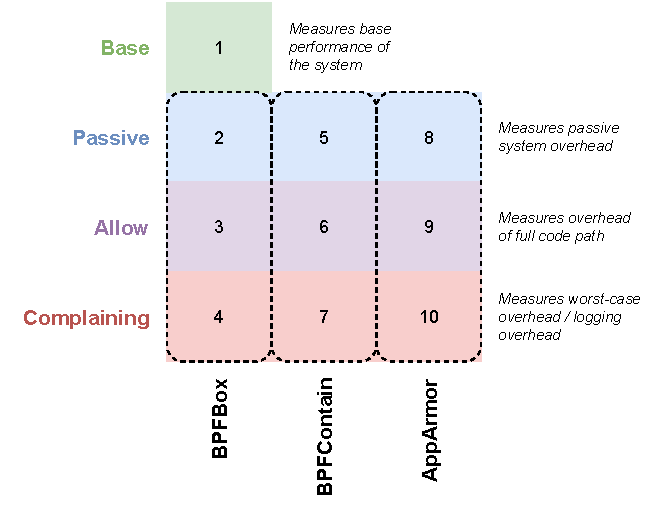
\includegraphics[width=0.8\linewidth]{figs/eval/configuration.pdf}
  \caption[Benchmarking system configurations]{
    The various system configurations used in the benchmarking tests.
  }%
  \label{fig:configuration}
\end{figure}

We consider ten system configurations in total (\Cref{fig:configuration}). The
\textbf{Base} configuration is the base system without any \glspl{lsm} or other
confinement primitives active or loaded in the kernel. The \textbf{\bpfbox},
\textbf{\bpfcontain}, and \textbf{AppArmor} configurations measure the performance
overhead of \bpfbox{}, \bpfcontain{}, and AppArmor, respectively. We then divide each of
these three configurations into three distinct test cases each. The \textbf{Passive} case
measures global system overhead without any active enforcement. The \textbf{Allow} case
measures active enforcement, allowing all security-sensitive operations. Finally, the
\textbf{Complain} case measures the worst-case overhead for each system, exercising the
full code path of each \gls{lsm} hook and logging every attempted access.

To ensure statistically valid results, we run each test at least eleven times, until
a standard deviation of at most $2\%$ of the mean is achieved. This is a sensible default
enforced by the Phoronix Test Suite to ensure statistically valid results. We also discard
the first run of each test to control for initial I/O transients. In total, the result is
at least ten trials for each test suite and system configuration. For reproducibility, we
make the benchmarking repository publicly available\footnote{Benchmarking tests are
available: \url{https://github.com/willfindlay/bpfcontain-benchmarks}}, including all
results and related scripts.

% \begin{inprogress}
%   \begin{itemize}
%     \item Test environment
%     \begin{itemize}
%       \item Describe system specs
%       \item To improve benchmark accuracy, we disable ...
%       \item We run tests in a privileged Docker container
%       \item Arch Linux Kernel 5.12.15-arch-1
%     \end{itemize}

%     \item Phoronix Test Suite tests
%     \begin{itemize}
%       \item \todo{Describe each test in detail and explain what LSM hooks it exercises}
%     \end{itemize}

%     \item \todo{Other tests if we have time}

%     \item Explain each test case (base, \{bpfbox, bpfcontain, apparmor\}, \{passive, allow, complaining\})
%     \item Run reach test for at least 11 trials, until we achieve an acceptable standard deviation ($<2\%$)
%     \item Discard first run of each trial, to control for initial I/O transients and caching
%     \item Reproducibility, give \bpfbox{} and \bpfcontain{} version, with tags on GitHub
%     \item Link to the benchmarking repo

%   \end{itemize}
% \end{inprogress}

\subsection{Results}%
\label{ss:eval-results}

This section presents the results of the OSBench micro-benchmarks (\Cref{fig:osbench} and
\Crefrange{tab:phoronix-create-files}{tab:phoronix-memory-allocations}) and the kernel
compilation (\Cref{fig:phoronix-kernel} and \Cref{tab:phoronix-kernel-compilation}) and
Apache web server (\Cref{fig:phoronix-apache} and \Cref{tab:phoronix-apache})
macro-benchmarks. We find that \bpfbox{} and \bpfcontain{} perform competitively with
AppArmor in many common use cases cases, with \bpfcontain{} experiencing performance
degradations in some cases, which can be attributed to \bpfcontain{}'s status as
a research prototype. In light of these results, we discuss how future optimizations to
\bpfcontain{} and the \gls{krsi} framework can greatly improve its performance overhead in
practice.

\begin{figure}[htp]
  \centering
  \subfloat{
    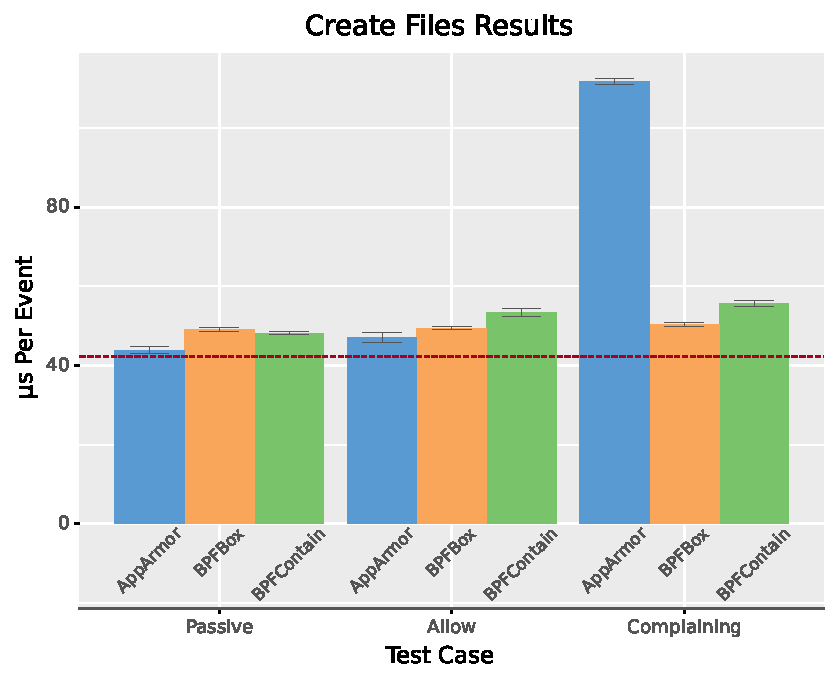
\includegraphics[width=0.45\linewidth]{results/graphs/Create-Files.pdf}%
  }\qquad
  \subfloat{
    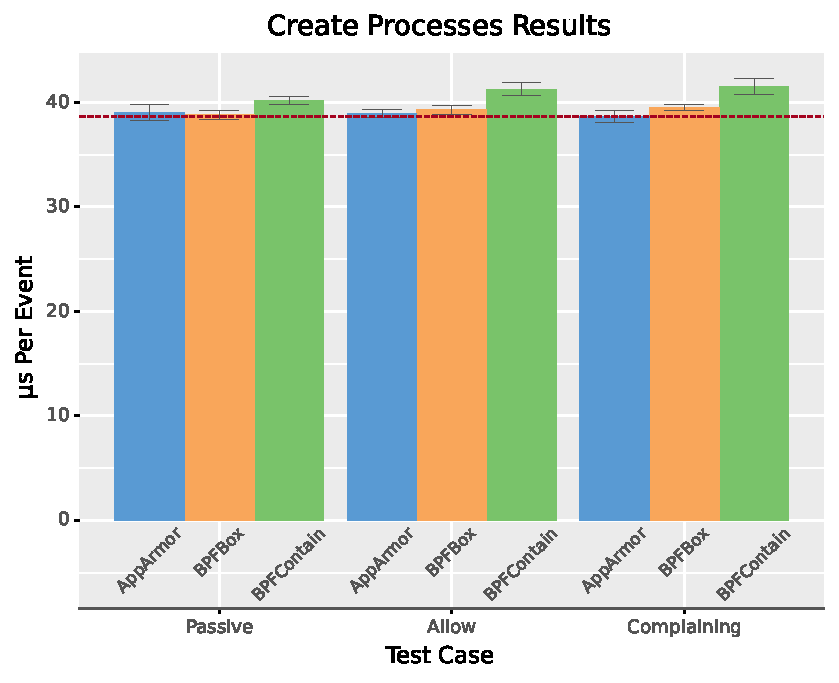
\includegraphics[width=0.45\linewidth]{results/graphs/Create-Processes.pdf}%
  }\\
  \subfloat{
    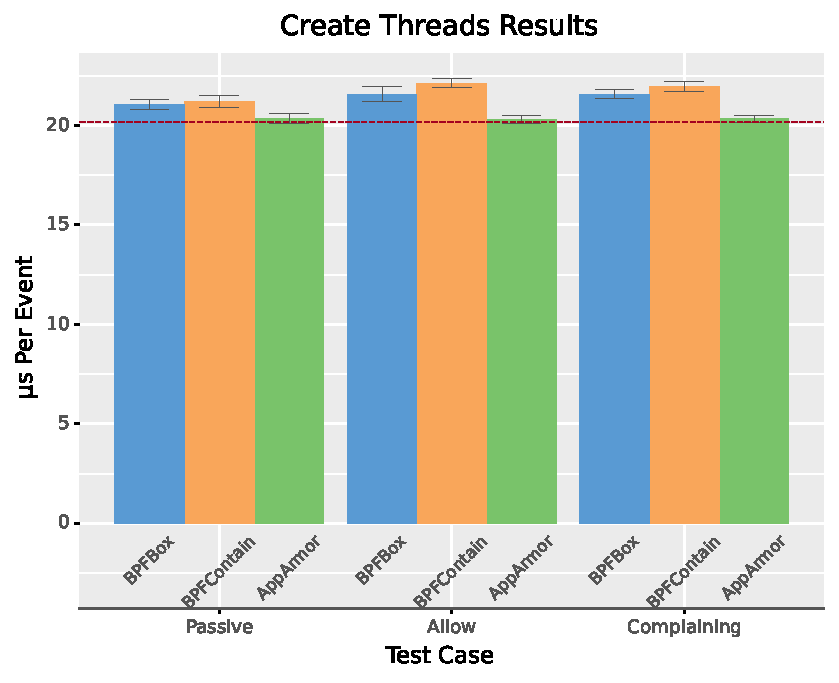
\includegraphics[width=0.45\linewidth]{results/graphs/Create-Threads.pdf}%
  }\qquad
  \subfloat{
    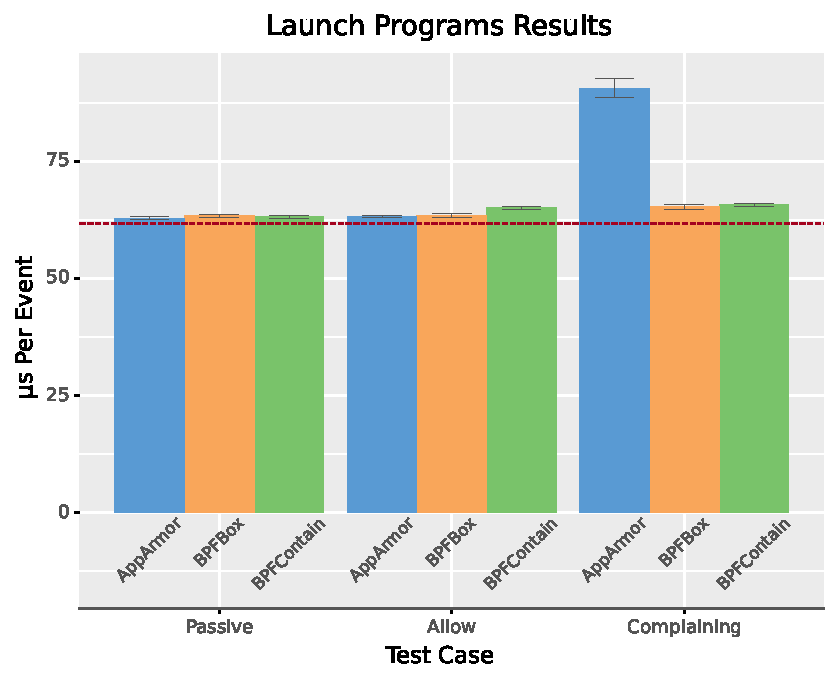
\includegraphics[width=0.45\linewidth]{results/graphs/Launch-Programs.pdf}%
  }\\
  \subfloat{
    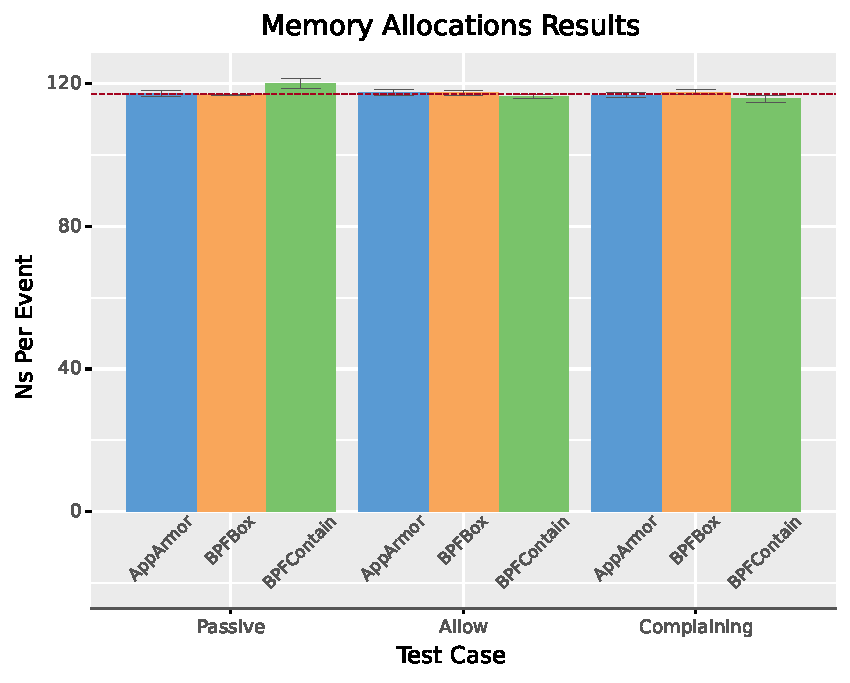
\includegraphics[width=0.45\linewidth]{results/graphs/Memory-Allocations.pdf}%
  }
  \caption[The results of the OSBench micro-benchmarks]{
    The results of the OSBench micro-benchmarks. The error bars show standard
    deviation and the red lines show base measurements for each test. Lower times are
    better.
  }%
  \label{fig:osbench}
\end{figure}

\subsubsection{OSBench File Creation}

The file creation benchmark (\Cref{tab:phoronix-create-files} and \Cref{fig:osbench}) indicates
that \bpfbox{} and \bpfcontain{} have significantly higher overhead than AppArmor in the
\textbf{Passive} and \textbf{Allow} cases. \bpfcontain{}, in particular, performs the worst
out of the three systems in these two cases. This poor performance can be
explained by the fact that it is an unoptimized research prototype, and that it performs
complex analysis on filesystem operations to come to a policy decision. Conversely,
AppArmor is a well-established security mechanism which has undergone significant
performance optimizations over time. Future optimizations on \bpfcontain{} can
significantly improve its performance overhead in practice. Despite a seemingly high
performance overhead in the \textbf{Passive} and \textbf{Allow} cases, \bpfbox{} and
\bpfcontain{} incur a performance penalty of under 12$\mu$s each, a slowdown which should
be acceptable in practice.  Moreover, in the \textbf{Complain} case, \bpfbox{} and
\bpfcontain{} significantly outperform AppArmor. This result can be attributed to
implementation differences in their event-logging mechanisms.

\begin{table}[htp!]
\centering
\footnotesize
\caption[Results of the create files benchmark]{Results of the create files benchmark. Units are $\mu$s Per Event. Lower is better. Percent overhead is compared to the baseline result.}
\label{tab:phoronix-create-files}
\begin{tabular}{llrrr}
\toprule
            &          &    Mean &   Std &  Overhead \\
Test Case & System &         &       &           \\
\midrule
Base & --- &   42.21 &  1.22 &       --- \\
\cline{1-5}
\multirow{3}{*}{Passive} & BPFBox &   49.09 &  0.40 &   16.31\% \\
            & BPFContain &   48.16 &  0.36 &   14.11\% \\
            & AppArmor &   43.87 &  0.95 &    3.93\% \\
\cline{1-5}
\multirow{3}{*}{Allow} & BPFBox &   49.41 &  0.39 &   17.08\% \\
            & BPFContain &   53.43 &  1.01 &   26.60\% \\
            & AppArmor &   47.07 &  1.15 &   11.52\% \\
\cline{1-5}
\multirow{3}{*}{Complaining} & BPFBox &   50.34 &  0.54 &   19.27\% \\
            & BPFContain &   55.67 &  0.75 &   31.89\% \\
            & AppArmor &  111.66 &  0.75 &  164.55\% \\
\bottomrule
\end{tabular}
\end{table}

% \begingroup\small
% \begin{longtable}[c]{llrrr}
%   \caption[Results of the file creation benchmark]{
%     Results of the file creation benchmark. Units are $\mu$s per event; lower is
%     better. Percent overhead is compared to the baseline result.
%   }%
%   \label{tab:phoronix-files}\\
%   \toprule
%    Test Case & System         &  Mean  & Std & Overhead (\%)\\
%    \midrule
%    Base      & ---            &  42.21 & 1.22 &  ---     \\
%    \midrule
%    Passive   & \bpfbox{}      &  49.09 & 0.40 &  16.31\% \\
%              & \bpfcontain{}  &  48.16 & 0.36 &  14.11\% \\
%              & AppArmor       &  43.87 & 0.95 &   3.93\% \\
%    \midrule
%    Allow     & \bpfbox{}      &  49.41 & 0.39 &  17.08\% \\
%              & \bpfcontain{}  &  53.43 & 1.01 &  26.60\% \\
%              & AppArmor       &  47.07 & 1.15 &  11.52\% \\
%    \midrule
%    Complain  & \bpfbox{}      &  50.34 & 0.54 &  19.27\% \\
%              & \bpfcontain{}  &  55.67 & 0.75 &  31.89\% \\
%              & AppArmor       & 111.66 & 0.75 & 164.55\% \\
%   \bottomrule
% \end{longtable}
% \endgroup

In the \textbf{Passive} case, \bpfbox{} and \bpfcontain{}'s high performance overhead can
be attributed to the fact that they each invoke multiple \gls{bpf} programs over multiple
\gls{lsm} hooks on the \texttt{open(2)}, \texttt{write(2)}, and \texttt{unlink(2)} code
paths. Unlike AppArmor, \bpfbox{} and \bpfcontain{} invoke a new \gls{ebpf} program on
every \gls{lsm} hook along this code path, then perform a map lookup to determine whether
the process is being actively traced. The overhead associated with this many \gls{bpf}
program invocations is non-trivial compared with the overhead of simply calling into an
\gls{lsm} hook. Future improvements to the \gls{krsi} framework may also be able to reduce
the performance overhead of \gls{bpf} \gls{lsm} programs.

In the \textbf{Allow} case, \bpfbox{} is more in line with AppArmor, while \bpfcontain{}
is shown to exhibit a slightly higher overhead. However, as with the \textbf{Passive}
case, this overhead should be acceptable in practice. We can attribute the additional
overhead shown by \bpfcontain{} to the nuances associated with its code path for file and
filesystem policies. For each file operation, \bpfcontain{} performs multiple map queries
and reads information from multiple kernel data structures to enforce its default policy.
Future iterations of \bpfcontain{} may improve this overhead by caching policy decisions
for filesystem objects and/or resolving inefficiencies in how \bpfcontain{} reads
information from kernel data structures.

In the \textbf{Complaining} case, \bpfbox{} and \bpfcontain{} significantly outperform
AppArmor, a fact which can be attributed to inefficiencies in AppArmor's logging
mechanism, which relies on the kernel's audit framework. The ring buffer maps used by
\bpfbox{} and \bpfcontain{} are known to exhibit comparatively less
overhead~\cite{zeng2015_auditing, zhang2021_lsm_file_overhead, nakryiko2020_ringbuf}.
Additional overhead may also arise due to differences in how AppArmor translates files and
access patterns to log messages.

\subsubsection{OSBench Process Creation}

The results of the process creation benchmark (\Cref{tab:phoronix-create-processes} and \Cref{fig:osbench}) indicate
that \bpfbox{} and \bpfcontain{} introduce modest overhead on top of the \texttt{fork(2)}
system call.  Comparatively, AppArmor introduces very little overhead, well within the
margin of error for measurements. The additional overhead introduced by \bpfbox{} and
\bpfcontain{} can be explained by the additional per-process and per-thread accounting
performed by each system. \bpfcontain{}, in particular, handles a significant amount of
per-process and per-thread metadata, which must be populated each time a \texttt{fork(2)}
or \texttt{clone(2)} occurs, and cleaned up each time a process exits. However, it should
be noted that both \bpfbox{} and \bpfcontain{} introduce less than $10\%$ overhead along
this code path (within 1--2$\mu$s), which should be imperceptible in practice.

% \begin{figure}[htp]
%   \centering
%   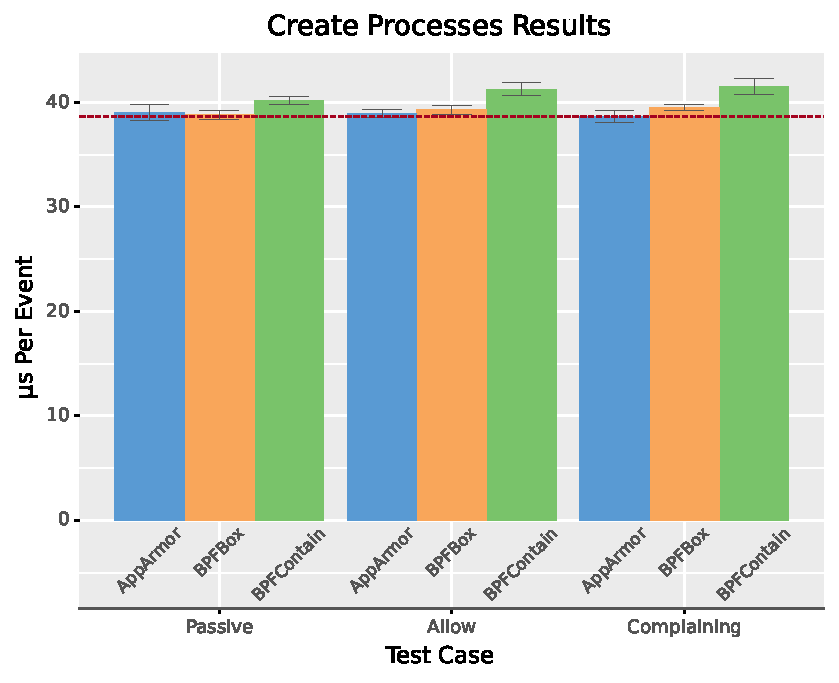
\includegraphics[width=0.8\linewidth]{results/graphs/Create-Processes.pdf}
%   \caption{
%     Results of the process creation benchmark.
%     The error bars show standard deviation and the red line shows the base measurement.
%     Lower times are better.
%   }%
%   \label{fig:phoronix-processes}
% \end{figure}

\begin{table}[htp!]
\centering
\footnotesize
\caption[Results of the create processes benchmark]{Results of the create processes benchmark. Units are $\mu$s Per Event. Lower is better. Percent overhead is compared to the baseline result.}
\label{tab:phoronix-create-processes}
\begin{tabular}{llrrr}
\toprule
            &          &   Mean &   Std & Overhead \\
Test Case & System &        &       &          \\
\midrule
Base & --- &  38.65 &  0.36 &      --- \\
\cline{1-5}
\multirow{3}{*}{Passive} & BPFBox &  38.81 &  0.44 &   0.40\% \\
            & BPFContain &  40.17 &  0.39 &   3.93\% \\
            & AppArmor &  39.04 &  0.74 &   1.01\% \\
\cline{1-5}
\multirow{3}{*}{Allow} & BPFBox &  39.28 &  0.41 &   1.63\% \\
            & BPFContain &  41.27 &  0.63 &   6.77\% \\
            & AppArmor &  38.94 &  0.34 &   0.74\% \\
\cline{1-5}
\multirow{3}{*}{Complaining} & BPFBox &  39.51 &  0.33 &   2.22\% \\
            & BPFContain &  41.49 &  0.76 &   7.33\% \\
            & AppArmor &  38.68 &  0.56 &   0.07\% \\
\bottomrule
\end{tabular}
\end{table}

% \begingroup\small
% \begin{longtable}[c]{llrrr}
%   \caption[Results of the process creation benchmark]{
%     Results of the process creation benchmark. Units are $\mu$s per event; lower is
%     better. Percent overhead is compared to the baseline result.
%   }%
%   \label{tab:phoronix-processes}\\
%   \toprule
%    Test Case & System         &  Mean & Std & Overhead (\%)\\
%    \midrule
%    Base      & ---            & 38.65 & 0.36 &  ---    \\
%    \midrule
%    Passive   & \bpfbox{}      & 38.81 & 0.44 &  0.40\% \\
%              & \bpfcontain{}  & 40.17 & 0.39 &  3.93\% \\
%              & AppArmor       & 39.04 & 0.74 &  1.01\% \\
%    \midrule
%    Allow     & \bpfbox{}      & 39.28 & 0.41 &  1.63\% \\
%              & \bpfcontain{}  & 41.27 & 0.63 &  6.77\% \\
%              & AppArmor       & 38.94 & 0.34 &  0.74\% \\
%    \midrule
%    Complain  & \bpfbox{}      & 39.51 & 0.33 &  2.22\% \\
%              & \bpfcontain{}  & 41.49 & 0.76 &  7.33\% \\
%              & AppArmor       & 38.68 & 0.56 &  0.07\% \\
%   \bottomrule
% \end{longtable}
% \endgroup

\subsubsection{OSBench Thread Creation}

The thread creation results (\Cref{tab:phoronix-create-threads} and \Cref{fig:osbench}) are directly related to the
process creation results discussed above, insofar as both operations exercise the same
\gls{bpf} programs in \bpfbox{} and \bpfcontain{}. Since thread creation is faster then
process creation, the percentage overhead of \bpfbox{} and \bpfcontain{} appear
comparatively higher, but the underlying delta is the same, at roughly 1--2$\mu$s per
event. Despite these differences in thread and process creation speeds, the resulting
percentage overhead of \bpfbox{} and \bpfcontain{} is still under 10\%.

% \begin{figure}[htp]
%   \centering
%   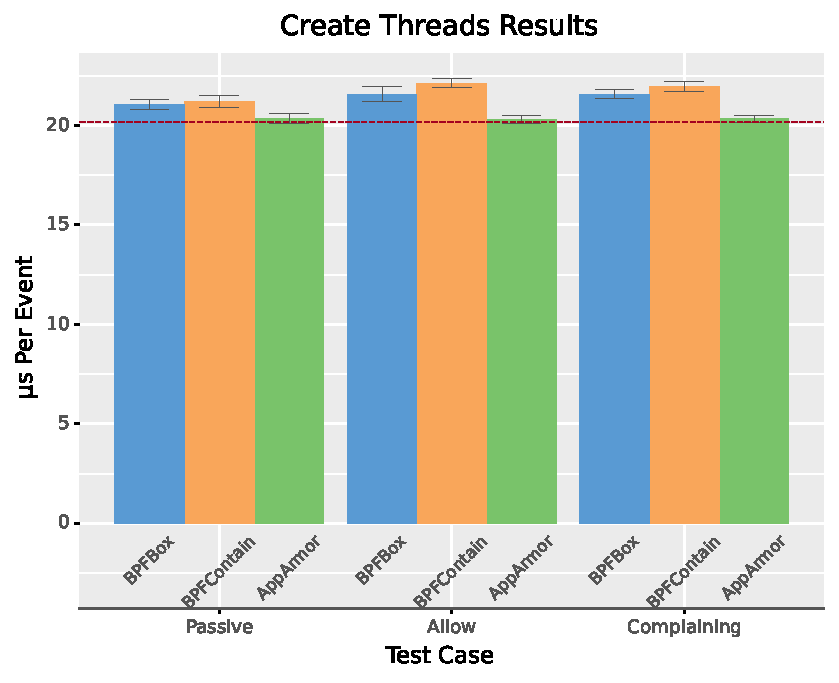
\includegraphics[width=0.8\linewidth]{results/graphs/Create-Threads.pdf}
%   \caption{
%     Results of the thread creation benchmark.
%     The error bars show standard deviation and the red line shows the base measurement.
%     Lower times are better.
%   }%
%   \label{fig:phoronix-threadsa}
% \end{figure}

\begin{table}[ht!]
\centering
\footnotesize
\caption[Results of the Create Threads benchmark]{Results of the Create Threads benchmark. Units are $\mu$s per event. Lower is better. Percent overhead is compared to the baseline result.}
\label{tab:phoronix-create-threads}
\begin{tabular}{llrrr}
\toprule
            &          &   Mean &   Std & Overhead \\
Test Case & System &        &       &          \\
\midrule
Base & --- &  20.18 &  0.19 &      --- \\
\cline{1-5}
\multirow{3}{*}{Passive} & BPFBox &  21.06 &  0.25 &   4.37\% \\
            & BPFContain &  21.21 &  0.30 &   5.08\% \\
            & AppArmor &  20.32 &  0.25 &   0.71\% \\
\cline{1-5}
\multirow{3}{*}{Allow} & BPFBox &  21.56 &  0.37 &   6.84\% \\
            & BPFContain &  22.11 &  0.22 &   9.53\% \\
            & AppArmor &  20.29 &  0.18 &   0.54\% \\
\cline{1-5}
\multirow{3}{*}{Complaining} & BPFBox &  21.57 &  0.25 &   6.90\% \\
            & BPFContain &  21.96 &  0.24 &   8.80\% \\
            & AppArmor &  20.32 &  0.16 &   0.70\% \\
\bottomrule
\end{tabular}
\end{table}

% \begingroup\small
% \begin{longtable}[c]{llrrr}
%   \caption[Results of the thread creation benchmark]{
%     Results of the thread creation benchmark. Units are $\mu$s per event; lower is
%     better. Percent overhead is compared to the baseline result.
%   }%
%   \label{tab:phoronix-threads}\\
%   \toprule
%    Test Case & System         &  Mean & Std  & Overhead (\%)\\
%    \midrule
%    Base      & ---            & 20.18 & 0.19 & ---     \\
%    \midrule
%    Passive   & \bpfbox{}      & 21.06 & 0.25 & 4.37\% \\
%              & \bpfcontain{}  & 21.21 & 0.30 & 5.08\% \\
%              & AppArmor       & 20.32 & 0.25 & 0.71\% \\
%    \midrule
%    Allow     & \bpfbox{}      & 21.56 & 0.37 & 6.84\% \\
%              & \bpfcontain{}  & 22.11 & 0.22 & 9.53\% \\
%              & AppArmor       & 20.29 & 0.18 & 0.54\% \\
%    \midrule
%    Complain  & \bpfbox{}      & 21.57 & 0.25 & 6.90\% \\
%              & \bpfcontain{}  & 21.96 & 0.24 & 8.80\% \\
%              & AppArmor       & 20.32 & 0.16 & 0.70\% \\
%   \bottomrule
% \end{longtable}
% \endgroup

\subsubsection{OSBench Program Launching}

The launch programs benchmark (\Cref{tab:phoronix-launch-programs} and \Cref{fig:osbench}) is essentially the
same as the process creation benchmark (c.f.~\Cref{tab:phoronix-create-processes}), with one
major difference: the addition of an \texttt{execve(2)} call after the \texttt{clone(2)}
system call. This \texttt{execve(2)} call adds a constant overhead of about 20$\mu$s on
top of the original process creation results, as well as additional \gls{lsm} hook
invocations along the \texttt{execve(2)} code path. These factors contribute to \bpfbox{}
and \bpfcontain{} performing slightly worse than AppArmor in the \textbf{Passive} and
\textbf{Allow} cases and significantly better than AppArmor in the \textbf{Complaining}
case.

The additional \gls{lsm} hook invocations caused by the \texttt{execve(2)} severely impact
AppArmor's performance in the \textbf{Complaining} case, for the same reasons as discussed
in the file creation results (c.f.~\Cref{tab:phoronix-create-files}). \bpfbox{} and \bpfcontain{}
exhibit comparatively little overhead, despite the \texttt{execve(2)} call. This result
can be explained by the fact that \texttt{execve(2)}'s code path invokes significantly
fewer \gls{lsm} hooks than the file creation and deletion code paths we examined earlier.
In all test cases, \bpfbox{} and \bpfcontain{} are able to achieve under $7\%$ overhead in
the worst case, and under $3\%$ in the majority of cases.

% \begin{figure}[htp]
%   \centering
%   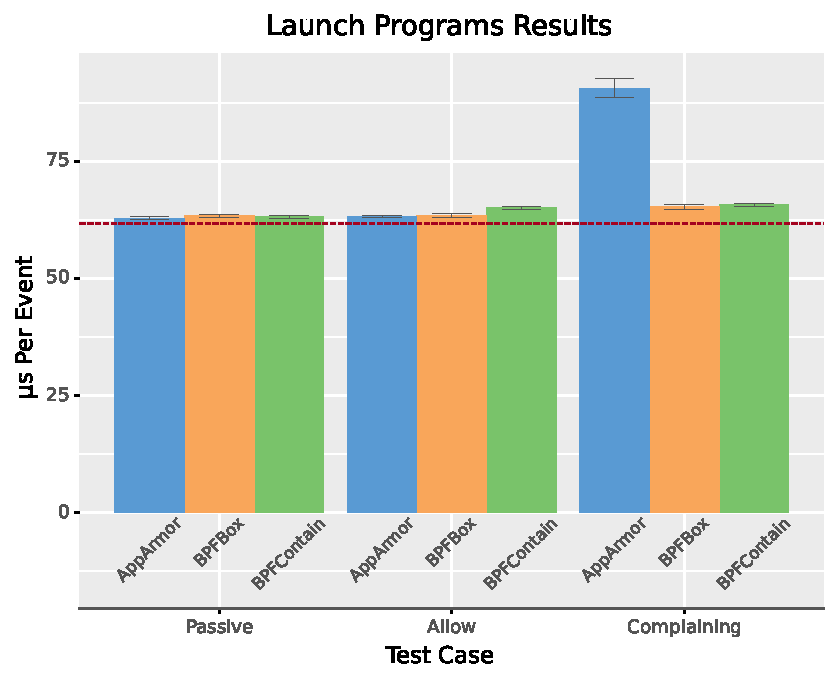
\includegraphics[width=0.8\linewidth]{results/graphs/Launch-Programs.pdf}
%   \caption{
%     Results of the program launching benchmark.
%     The error bars show standard deviation and the red line shows the base measurement.
%     Lower times are better.
%   }%
%   \label{fig:phoronix-launch-programs}
% \end{figure}

\begin{table}[htp!]
\centering
\footnotesize
\caption[Results of the launch programs benchmark]{Results of the launch programs benchmark. Units are $\mu$s Per Event. Lower is better. Percent overhead is compared to the baseline result.}
\label{tab:phoronix-launch-programs}
\begin{tabular}{llrrr}
\toprule
            &          &   Mean &   Std & Overhead \\
Test Case & System &        &       &          \\
\midrule
Base & --- &  61.67 &  0.20 &      --- \\
\cline{1-5}
\multirow{3}{*}{Passive} & BPFBox &  63.30 &  0.28 &   2.64\% \\
            & BPFContain &  63.12 &  0.28 &   2.34\% \\
            & AppArmor &  62.84 &  0.25 &   1.89\% \\
\cline{1-5}
\multirow{3}{*}{Allow} & BPFBox &  63.44 &  0.40 &   2.86\% \\
            & BPFContain &  65.05 &  0.38 &   5.47\% \\
            & AppArmor &  63.17 &  0.21 &   2.43\% \\
\cline{1-5}
\multirow{3}{*}{Complaining} & BPFBox &  65.22 &  0.48 &   5.75\% \\
            & BPFContain &  65.66 &  0.30 &   6.47\% \\
            & AppArmor &  90.56 &  1.97 &  46.83\% \\
\bottomrule
\end{tabular}
\end{table}

% \begingroup\small
% \begin{longtable}[c]{llrrr}
%   \caption[Results of the program launching benchmark]{
%     Results of the program launching benchmark. Units are $\mu$s per event; lower is
%     better. Percent overhead is compared to the baseline result.
%   }%
%   \label{tab:phoronix-launch-programs}\\
%   \toprule
%    Test Case & System         &  Mean & Std  & Overhead (\%)\\
%    \midrule
%    Base      & ---            & 61.67 & 0.20 & ---     \\
%    \midrule
%    Passive   & \bpfbox{}      & 63.30 & 0.28 & 2.64 \% \\
%              & \bpfcontain{}  & 63.12 & 0.28 & 2.34 \% \\
%              & AppArmor       & 62.84 & 0.25 & 1.89 \% \\
%    \midrule
%    Allow     & \bpfbox{}      & 63.44 & 0.40 & 2.86 \% \\
%              & \bpfcontain{}  & 65.05 & 0.38 & 5.47 \% \\
%              & AppArmor       & 63.17 & 0.21 & 2.43 \% \\
%    \midrule
%    Complain  & \bpfbox{}      & 65.22 & 0.48 & 5.75 \% \\
%              & \bpfcontain{}  & 65.66 & 0.30 & 6.47 \% \\
%              & AppArmor       & 90.56 & 1.97 & 46.83\% \\
%   \bottomrule
% \end{longtable}
% \endgroup

\subsubsection{OSBench Memory Allocations}

The memory allocation benchmark (\Cref{tab:phoronix-memory-allocations} and
\Cref{fig:osbench}) indicates that none of the systems had any significant affect on
memory allocation. In some cases, percent overhead falsely appears to indicate
a performance \textit{improvement}, which we attribute to measurement error rather than
any indication of increased performance. This result is consistent with expectations,
since memory allocation does not directly interact with any \gls{lsm} hooks in the kernel,
and neither \bpfbox{} nor \bpfcontain{} instruments any \gls{bpf} programs on the heap
allocation code path.

\begin{table}[ht!]
\centering
\footnotesize
\caption[Results of the Memory Allocations benchmark]{Results of the Memory Allocations benchmark. Units are ns per event. Lower is better. Percent overhead is compared to the baseline result.}
\label{tab:phoronix-memory-allocations}
\begin{tabular}{llrrr}
\toprule
            &          &    Mean &   Std & Overhead \\
Test Case & System &         &       &          \\
\midrule
Base & --- &  117.17 &  0.67 &      --- \\
\cline{1-5}
\multirow{3}{*}{Passive} & BPFBox &  116.87 &  0.18 &  -0.26\% \\
            & BPFContain &  120.05 &  1.27 &   2.46\% \\
            & AppArmor &  117.24 &  0.97 &   0.06\% \\
\cline{1-5}
\multirow{3}{*}{Allow} & BPFBox &  117.41 &  0.71 &   0.21\% \\
            & BPFContain &  116.42 &  0.62 &  -0.64\% \\
            & AppArmor &  117.49 &  0.81 &   0.28\% \\
\cline{1-5}
\multirow{3}{*}{Complaining} & BPFBox &  117.62 &  0.75 &   0.38\% \\
            & BPFContain &  115.73 &  1.04 &  -1.22\% \\
            & AppArmor &  116.81 &  0.80 &  -0.31\% \\
\bottomrule
\end{tabular}
\end{table}


% \begin{figure}[htp]
%   \centering
%   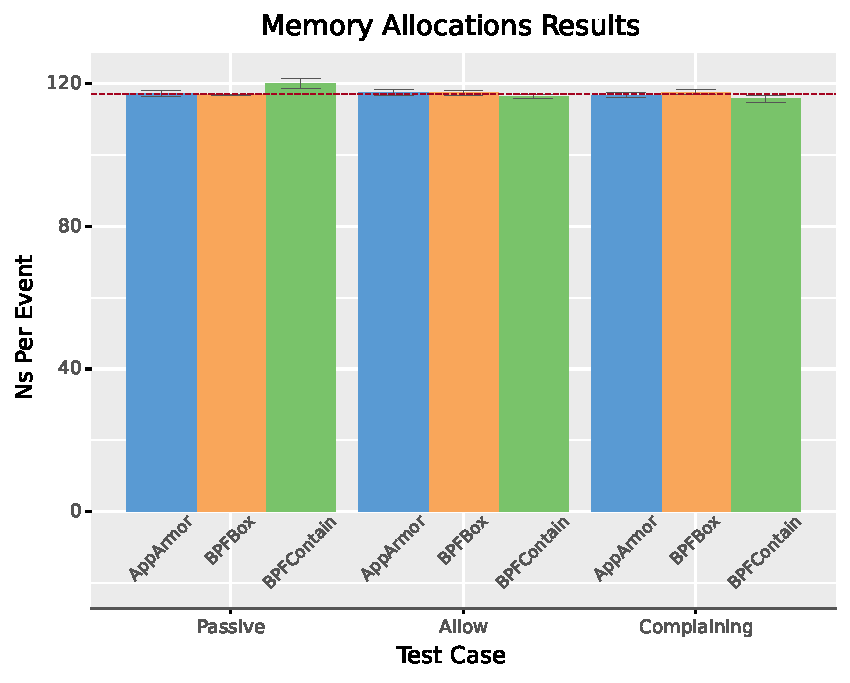
\includegraphics[width=0.8\linewidth]{results/graphs/Memory-Allocations.pdf}
%   \caption{
%     Results of the memory allocation benchmark.
%     The error bars show standard deviation and the red line shows the base measurement.
%     Lower times are better.
%   }%
%   \label{fig:phoronix-memory}
% \end{figure}
% \begingroup\small
% \begin{longtable}[c]{llrrr}
%   \caption[Results of the memory allocation benchmark]{
%     Results of the memory allocation benchmark. Units are Ns per event; lower is
%     better. Percent overhead is compared to the baseline result.
%   }%
%   \label{tab:phoronix-memory}\\
%   \toprule
%    Test Case & System         &  Mean  & Std  & Overhead (\%)\\
%    \midrule
%    Base      & ---            & 117.17 & 0.67 & ---     \\
%    \midrule
%    Passive   & \bpfbox{}      & 116.87 & 0.18 & -0.26\% \\
%              & \bpfcontain{}  & 120.05 & 1.27 &  2.46\% \\
%              & AppArmor       & 117.24 & 0.97 &  0.06\% \\
%    \midrule
%    Allow     & \bpfbox{}      & 117.41 & 0.71 &  0.21\% \\
%              & \bpfcontain{}  & 116.42 & 0.62 & -0.64\% \\
%              & AppArmor       & 117.49 & 0.81 &  0.28\% \\
%    \midrule
%    Complain  & \bpfbox{}      & 117.62 & 0.75 &  0.38\% \\
%              & \bpfcontain{}  & 115.73 & 1.04 & -1.22\% \\
%              & AppArmor       & 116.81 & 0.80 & -0.31\% \\
%   \bottomrule
% \end{longtable}
% \endgroup


\subsubsection{Kernel Compilation Results}

The kernel compilation benchmark (\Cref{tab:phoronix-kernel-compilation} and
\Cref{fig:phoronix-kernel}) provides a representative depiction of overhead for
a computationally-heavy task that involves multiple processes and significant amounts of
file I/O. The results of this benchmark indicate that \bpfbox{} and \bpfcontain{} exhibit
performance overhead that is roughly consistent with AppArmor in the average case. The
\textbf{Passive} and \textbf{Allow} results indicate that all three systems exhibit an
acceptable performance overhead of under about $3\%$. The \textbf{Complain} results
indicate that \bpfcontain{} performs significantly better than both \bpfbox{} and AppArmor
under a large event logging volume. This result can be attributed to minor implementation
details, including improvements in how \bpfcontain{} handles event logging from multiple
distinct sources.
%This result can likely be
%attributed to \bpfcontain{}'s more efficient userspace implementation in Rust, which
%significantly outperforms the \bpfbox{} Python implementation.

\begin{table}[htp!]
\centering
\footnotesize
\caption[Results of the kernel compilation benchmark]{Results of the kernel compilation benchmark. Units are Seconds. Lower is better. Percent overhead is compared to the baseline result.}
\label{tab:phoronix-kernel-compilation}
\begin{tabular}{llrrr}
\toprule
            &          &    Mean &   Std & Overhead \\
Test Case & System &         &       &          \\
\midrule
Base & --- &  235.32 &  1.96 &      --- \\
\cline{1-5}
\multirow{3}{*}{Passive} & BPFBox &  237.95 &  1.88 &   1.12\% \\
            & BPFContain &  237.63 &  2.08 &   0.98\% \\
            & AppArmor &  236.45 &  1.92 &   0.48\% \\
\cline{1-5}
\multirow{3}{*}{Allow} & BPFBox &  238.23 &  2.19 &   1.24\% \\
            & BPFContain &  243.09 &  2.19 &   3.30\% \\
            & AppArmor &  237.59 &  2.04 &   0.97\% \\
\cline{1-5}
\multirow{3}{*}{Complaining} & BPFBox &  269.64 &  1.98 &  14.59\% \\
            & BPFContain &  244.80 &  2.04 &   4.03\% \\
            & AppArmor &  288.54 &  2.11 &  22.62\% \\
\bottomrule
\end{tabular}
\end{table}


\begin{table}[ht!]
\centering
\footnotesize
\caption[Results of the Apache benchmark]{Results of the Apache benchmark. Units are requests per second. Higher is better. Percent overhead is compared to the baseline result.}
\label{tab:phoronix-apache}
\begin{tabular}{llrrr}
\toprule
            &          &      Mean &     Std & Overhead \\
Test Case & System &           &         &          \\
\midrule
Base & --- &  20576.49 &  281.94 &      --- \\
\cline{1-5}
\multirow{3}{*}{Passive} & BPFBox &  19946.04 &  233.62 &   3.06\% \\
            & BPFContain &  19530.92 &  317.95 &   5.08\% \\
            & AppArmor &  20363.42 &  331.64 &   1.04\% \\
\cline{1-5}
\multirow{3}{*}{Allow} & BPFBox &  19465.86 &  253.81 &   5.40\% \\
            & BPFContain &  18934.55 &  299.23 &   7.98\% \\
            & AppArmor &  20276.95 &   64.30 &   1.46\% \\
\cline{1-5}
\multirow{3}{*}{Complaining} & BPFBox &  20139.10 &  101.59 &   2.13\% \\
            & BPFContain &  18293.09 &  160.00 &  11.10\% \\
            & AppArmor &  19827.05 &  298.27 &   3.64\% \\
\bottomrule
\end{tabular}
\end{table}

% \begingroup\small
% \begin{longtable}[c]{llrrr}
%   \caption[Results of the kernel compilation benchmark]{
%     Results of the kernel compilation benchmark. Units are seconds to compile; lower is
%     better. Percent overhead is compared to the baseline result.
%   }%
%   \label{tab:phoronix-kernel}\\
%   \toprule
%    Test Case & System         &  Mean  & Std  & Overhead (\%)\\
%    \midrule
%    Base      & ---            & 235.32 & 1.96 & ---     \\
%    \midrule
%    Passive   & \bpfbox{}      & 237.95 & 1.88 &  1.12\% \\
%              & \bpfcontain{}  & 237.63 & 2.08 &  0.98\% \\
%              & AppArmor       & 236.45 & 1.92 &  0.48\% \\
%    \midrule
%    Allow     & \bpfbox{}      & 238.23 & 2.19 &  1.24\% \\
%              & \bpfcontain{}  & 243.09 & 2.19 &  3.30\% \\
%              & AppArmor       & 237.59 & 2.04 &  0.97\% \\
%    \midrule
%    Complain  & \bpfbox{}      & 269.64 & 1.98 & 14.59\% \\
%              & \bpfcontain{}  & 244.81 & 2.04 &  4.03\% \\
%              & AppArmor       & 288.54 & 2.11 & 22.62\% \\
%   \bottomrule
% \end{longtable}
% \endgroup

\begin{figure}[htp]
  \centering
  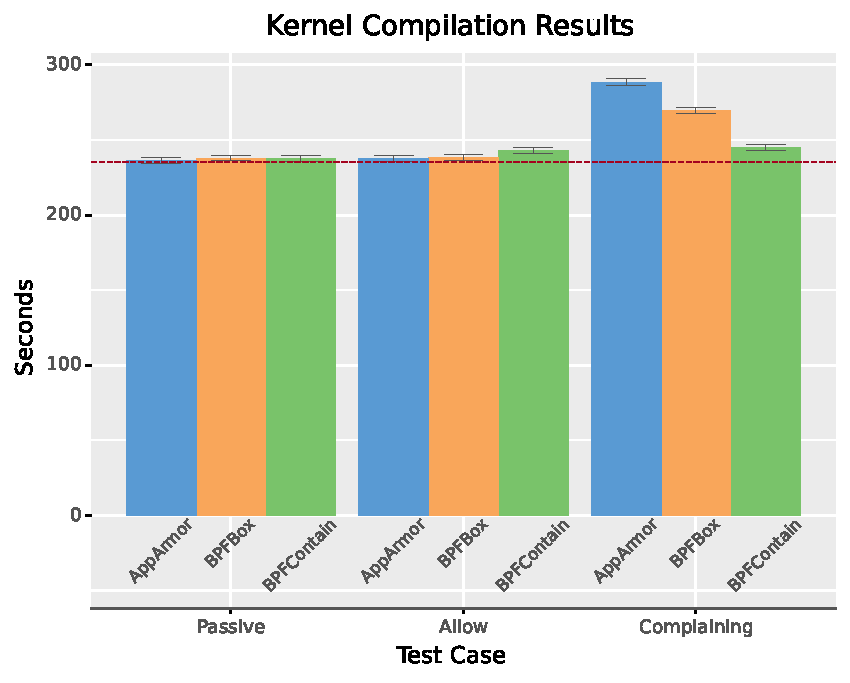
\includegraphics[width=0.6\linewidth]{results/graphs/Kernel-Compilation.pdf}
  \caption[Results of the kernel compilation benchmark]{
    Results of the kernel compilation benchmark.
    The error bars show standard deviation and the red line shows the base measurement.
    Lower times are better.
  }%
  \label{fig:phoronix-kernel}
\end{figure}

\begin{figure}[htp]
  \centering
  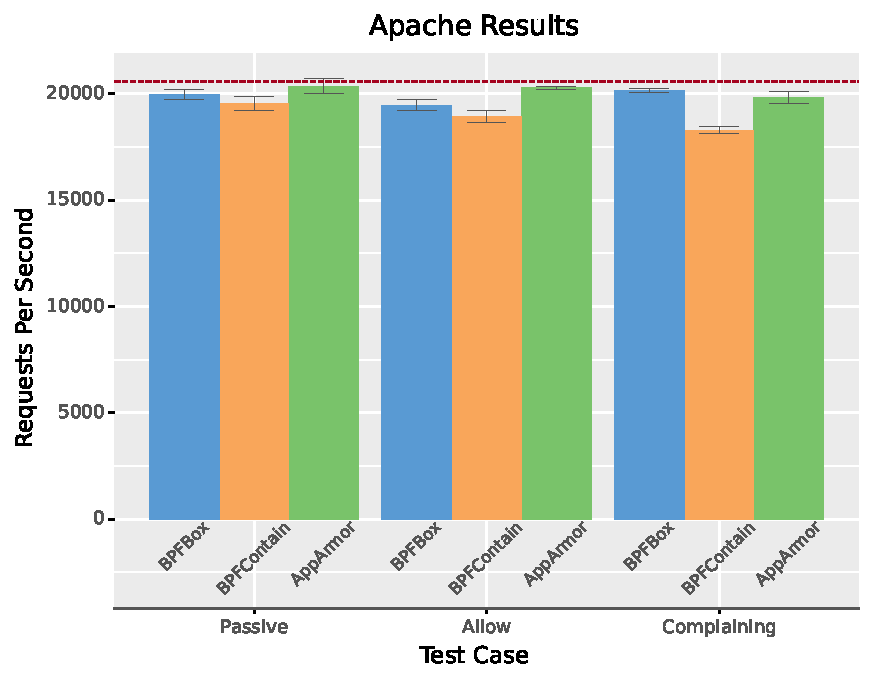
\includegraphics[width=0.6\linewidth]{results/graphs/Apache.pdf}
  \caption[Results of the Apache web server benchmark]{
    Results of the Apache web server benchmark.
    The error bars show standard deviation and the red line shows the base measurement.
    Higher requests per second are better.
  }%
  \label{fig:phoronix-apache}
\end{figure}


\subsubsection{Apache Web Server Results}

The Apache web server benchmark (\Cref{tab:phoronix-apache} and \Cref{fig:phoronix-apache}) indicates that, while
\bpfbox{} and \bpfcontain{} do exhibit a higher performance overhead than AppArmor, this
overhead is still within an acceptable range at around $11\%$ in the worst case for
\bpfcontain{}. This overhead should still be quite acceptable in practice, and can be
improved through further optimizations in \bpfcontain{}'s enforcement engine, which is
still in the prototype phase. The results from the \textbf{Complain} case appear to
indicate a slight performance improvement for \bpfbox{} over AppArmor; this is likely due
to variance in the measurements rather than a true performance improvement, as the
difference between the two systems falls within the margin of error.

% \begingroup\small
% \begin{longtable}[c]{llrrr}
%   \caption[Results of the Apache web server benchmark]{
%     Results of the Apache web server benchmark. Units are requests per second; higher is
%     better. Percent overhead is compared to the baseline result.
%   }%
%   \label{tab:phoronix-apache}\\
%   \toprule
%    Test Case & System         &  Mean   & Std   & Overhead (\%)\\
%    \midrule
%    Base      & ---            & 20576.49 & 281.94 & ---     \\
%    \midrule
%    Passive   & \bpfbox{}      & 19946.04 & 233.62 &  3.06\% \\
%              & \bpfcontain{}  & 19530.92 & 317.95 &  5.08\% \\
%              & AppArmor       & 20363.42 & 331.64 &  1.04\% \\
%    \midrule
%    Allow     & \bpfbox{}      & 19465.86 & 253.81 &  5.40\% \\
%              & \bpfcontain{}  & 18934.55 & 299.23 &  7.98\% \\
%              & AppArmor       & 20276.95 &  64.30 &  1.46\% \\
%    \midrule
%    Complain  & \bpfbox{}      & 20139.10 & 101.59 &  2.13\% \\
%              & \bpfcontain{}  & 18293.09 & 160.00 & 11.10\% \\
%              & AppArmor       & 19827.05 & 298.27 &  3.64\% \\
%   \bottomrule
% \end{longtable}
% \endgroup

% \subsubsection{\glsentryshort{ipc} Results}

\subsection{Discussion of Results}%
\label{ss:eval-performance-discussion}

The results of the benchmarking tests show that both \bpfbox{} and \bpfcontain{} incur
acceptable performance overhead in practice. In many cases, overhead is competitive with
AppArmor, a standard \gls{lsm} that ships with the stock Linux kernel. In other cases, the
performance overhead of \bpfbox{} and \bpfcontain{} is higher than that of AppArmor, but
still within an acceptable range, such that the slowdown should be either imperceptible or
acceptable in most practical use cases.  As \bpfbox{} and \bpfcontain{} are both research
prototypes, they have not yet been optimized to the extent that AppArmor has. This lack of
optimization is particularly evident in the results for \bpfcontain{}, and may account for
significant differences in performance in the file I/O and Apache web server tests.

\begin{table}[ht]
  \centering
  \footnotesize
  \caption[Geometric means of Phoronix benchmarking results]{
    Geometric means of Phoronix benchmarking results, as provided by the Phoronix Test
    Suite. These are indicative of overall performance across all tests. For test case,
    percent change from the base results are also given. Higher values are better.
  }%
  \label{tab:phoronix-geometric}
  \begin{tabular}{llrr}
  \toprule
             &               & Geom. Mean & Overhead (\%)\\
   Test Case & System        &            &              \\
   \midrule
   Base      &               & 6.238          & --- \\
   \cline{1-4}
   Passive   & \bpfbox{}     & 6.007          & 3.70\% \\
             & \bpfcontain{} & 5.951          & 4.60\% \\
             & AppArmor      & 6.158          & 1.28\% \\
   \cline{1-4}
   Allow     & \bpfbox{}     & 5.944          & 4.71\% \\
             & \bpfcontain{} & 5.763          & 7.61\% \\
             & AppArmor      & 6.086          & 2.35\% \\
   \cline{1-4}
   Complain  & \bpfbox{}     & 5.823          & 6.65\% \\
             & \bpfcontain{} & 5.693          & 8.74\% \\
             & AppArmor      & 4.962          & 20.46\% \\
  \bottomrule
  \end{tabular}
\end{table}

While \bpfbox{} and \bpfcontain{} are not as efficient as AppArmor in the \textbf{Passive}
and \textbf{Allow}  test cases, the additional performance overhead should be an
acceptable price to pay for the increase in flexibility and system observability afforded
by an \gls{ebpf} implementation as opposed to a traditional Linux Security Module.
Moreover, \bpfcontain{} extends \bpfbox{}'s original enforcement model, adding new rule categories
and enforcement defaults. While these enhancements may be the cause of some additional
performance overhead, we attribute the majority of \bpfcontain{}'s actual performance
overhead to sub-optimal memory allocations and data structure access patterns, which can
be optimized in the future.

Despite under-performing in the \textbf{Passive} and \textbf{Allow} cases, both \bpfbox{}
and \bpfcontain{} significantly outperform AppArmor in the \textbf{Complain} test case,
due to a more efficient event logging mechanism.  \Cref{tab:phoronix-geometric} shows the
geometric mean of all tests for each test case, indicating that \bpfbox{} and
\bpfcontain{} exhibit and average performance penalty of under $9\%$ in practice, while
AppArmor can exhibit overheads of up to $20\%$ in the worst case.

Although the results presented in this section indicate a comparative performance with
AppArmor, many other widely-adopted \glspl{lsm} can perform significantly worse than
AppArmor in some cases. For instance, Zhang \etal~\cite{zhang2021_lsm_file_overhead} found
that SELinux, perhaps the most widely-used Linux \gls{mac} implementation, exhibits
significant performance overhead, many times worse than AppArmor in some cases. These
results could indicate that \bpfbox{} and \bpfcontain{} might perform favourably compared
to alternative \glspl{lsm} like SELinux, although further investigation is needed in order
to establish a direct comparison.

\section{Security Analysis}%
\label{s:eval-security}

We now turn our attention to the security of \bpfbox{} and \bpfcontain. Specifically, we
conduct an informal security analysis on both systems, evaluating how well they are able
to confine an attacker under the threat model presented in \Cref{s:cp-threat-model} of
\Cref{c:confinement-problem}. In particular, we examine the various policy rule categories
provided by both \bpfbox{} and \bpfcontain{} as well as how their respective enforcement
engines enforce policy at runtime. We characterize an adversary's ability to escape
confinement based on whether the adversary is able to violate the security assumptions of
\bpfbox{} and \bpfcontain{} under a policy designed to prevent such violations.

% \todo{The plan for this section is to first revisit the threat model, then go through each
% policy \enquote{category} supported by \bpfbox{} and \bpfcontain{}. In a few categories
% (IPC, capabilities, kernel interfaces) \bpfcontain{} is just better... The \bpfbox{}
% prototype left some of this stuff out, and some of it is much weaker. In the networking
% category, both \bpfbox{} and \bpfcontain{} have room for improvement. We can do a forward
% ref to limitations / future work for this.}

\subsection{Threat Model Revisited}

Recall the threat model presented in \Cref{s:cp-threat-model} of
\Cref{c:confinement-problem}. We assume a remote adversary who is confined by some policy
$\mathcal{P}$. The adversary's goal is to escape confinement by circumventing
$\mathcal{P}$, enabling them to access sensitive resources, interfere or tamper with the
system, or perform other unauthorized actions. Our goal is to confine the adversary,
limiting the set of all actions they can perform to some subset of allowed actions. We
express such confinement using the policy $\mathcal{P}$ which defines rules governing the
set of operations some subject $\mathcal{S}_i$ may perform on system objects
$\mathcal{O}_1 \mathellipsis \mathcal{O}_n$. To enforce our confinement policy, we rely on
a \textit{confinement engine} which has been loaded into the kernel's reference monitor.

Under our threat model, we assign significant capabilities to the adversary. Aside from the
restrictions imposed by our confinement policy, we assume that they have root-level access
to the system, including the ability to load code into the kernel, bypass discretionary
access controls, read or modify any persistent resource, and establish persistent access
to the system. Thus, an attacker that is able to escape or bypass confinement has
effectively compromised the entire system. Further, our enforcement engine must take steps
protect itself, preventing the attacker from simply loading or modifying code in the
kernel, which would result in the ability to tamper with or bypass the enforcement engine.

In the subsections that follow, we consider four broad access categories and describe how
\bpfbox{} and \bpfcontain{}'s confinement policy and enforcement engine prevent attacks
related to these access categories. In some cases, the original \bpfbox{} policy
specification (as presented in this thesis) provided insufficient protection against
specific access patterns. In these instances, we describe how \bpfcontain{} improves upon
the original \bpfbox{} design.

\subsection{Files, Filesystems, and Kernel Interfaces}

Correct mediation of file and filesystem accesses is critical to ensure that an adversary
is confined. Files define the canonical persistent data store in modern \gls{cots}
operating systems, including Linux. Depending on the nature of the file, the information
stored within may be confidential, security-sensitive, or otherwise critical to normal
system operation. Attacker modification of persistent files is often the first step in
mounting a Confused Deputy attack~\cite{hardy1988_confused_deputy}, along with other
classes of attack such as data corruption, information disclosure, and memory safety
attacks.

Under the Unix model, special files and filesystems define an entrypoint into kernel
interfaces, many of which are security-sensitive. For example, character devices expose an
interface into device drivers, while special filesystems like \texttt{sysfs} and
\texttt{securityfs} expose behavioural parameters and export sensitive information such as
the system memory map. Limiting access to these files is of paramount importance, since
unrestricted access could enable an attacker to change the behaviour of the kernel, read
sensitive information, or modify global system parameters.

\subsubsection{\bpfbox{}}

To confine a process' access to the filesystem, \bpfbox{} supports \enquote{file} rules,
which take a pathname and corresponding access vector. This access vector encodes the
specific file operations that a process can perform on the file. Since \bpfbox{} policies
are default-deny, an adversary running under a \bpfbox{} confinement policy should be
unable to perform an operation $Op_i$ on any file $F_j$ unless this operation is
explicitly covered under a file rule. For the purposes of confinement, \bpfbox{} treats
all files equally, regardless of whether the file is a special file or belongs to
a special filesystem. Thus, any access to any file on the system is governed by the same
set of file rules. The only exception to this is a special \enquote{proc} rule which
enables a policy to define access to per-pid \texttt{procfs} entries belonging to another
process.

To enforce its file policy, the \bpfbox{} enforcement engine instruments \gls{ebpf}
programs on several \gls{lsm} hooks, including inode-based, file-based, and path-based
hooks. Taken together, these hooks provide complete mediation over the set of all file
operations, by instrumenting access at the \gls{vfs} layer. \bpfbox{} encodes its file
policy using an \gls{ebpf} map, taking the inode and device numbers associated with a file
and its filesystem as a key. When a process requests access to a file, \bpfbox{} computes
a key for that file and makes a query against its policy map. This technique has a natural
side effect of eliminating \gls{toctou} race conditions on a file's pathname, since inodes
are resolved at policy load time.

Despite being effective, \bpfbox{}'s inode resolution strategy is subject to a few
fundamental limitations. Since inode's are resolved at policy load time, \bpfbox{} traces
the confined process, granting implicit access to any files that the process creates
during its lifecycle.  An attack against this model would consist of unlinking and
re-creating a file after a policy has been loaded, causing \bpfbox{} to see it as
a different file when enforcing access control. In the worst case, this is effectively
a denial of service against the confined process, since \bpfbox{} enforces a default-deny
policy on unrecognized files.  This attack would also require the adversary to be
unconfined, such that they would be able to perform the necessary operations on the file.

\subsubsection{\bpfcontain{}}

Like \bpfbox{}, \bpfcontain{} supports file rules that specify a target pathname and
corresponding access vector. In addition to file rules, \bpfcontain{} also supports
filesystem rules for defining per-filesystem policy. A filesystem rule can be thought of
as a coarser-grained version of a file rule, specifying access at the per-filesystem
rather than the per-file level. In order to ensure mediation over explicit denials,
\bpfcontain{} always prioritizes fine-grained file rules over coarse-grained filesystem
rules. This prevents a policy from inadvertently obviating its own file rules with
a careless filesystem rule.

Due to current limitations of \gls{ebpf}, \bpfcontain{} currently uses the same inode
resolution strategy as \bpfbox{}. The strengths and weaknesses of this technique are the
same as in \bpfbox{}, with no major differences. However, future versions of \bpfcontain{}
may move to runtime path-based resolution, once the kernel offers better support for
string helpers and unbounded loops.

Unlike \bpfbox{}, \bpfcontain{} treats regular files differently from special files and
special filesystems. This improves security, as not only do special files and filesystems
have different semantics from regular files, but they also directly expose interfaces into
(potentially untrusted) kernel code. Rather than resolving special files by inode and
filesystem number, \bpfcontain{} looks at their major and minor number pair. Taken
together, these two numbers always uniquely identify a special file, regardless of when it
was created or whether it exists in multiple places at once. This resolution strategy is
not vulnerable to the same attack as the inode resolution strategy, since the adversary
cannot control a device's major and minor number.

Rather than being outright default-deny, \bpfcontain{} uses heuristics to determine the
appropriate default policy action on system objects. In the case of regular files,
\bpfcontain{} checks to see whether the filesystem superblock is a part of the container's
user namespace (provided that namespace is not the global namespace). If it is, the
filesystem was mounted within the context of the container, and so it is safe to allow
access. Otherwise, access is denied. Since special files and filesystems can be
significantly more dangerous, \bpfcontain{} assumes a default-deny policy instead. This
strategy allows \bpfcontain{} to (under certain conditions) relax requirements on policy
authors, without sacrificing security.

\subsection{POSIX Capabilities and Privileged System Calls}

Under Linux, POSIX capabilities~\cite{posix_capabilities} define a process' ability to
override discretionary access controls and access certain privileged kernel interfaces.
Although these cannot be used to override mandatory access controls (such as those
enforced by \bpfbox{} and \bpfcontain{}), they still provide a means of limiting the power
of the root user. This becomes particularly evident in the case of privileged kernel
interfaces, which can affect global system state or enable an attacker to load untrusted
code into the kernel.

\subsubsection{\bpfbox{}}

The \bpfbox{} prototype presented in this thesis does not directly interact with POSIX
capabilities in any way. Instead, \bpfbox{} denies access to system resources using its
\gls{lsm} hooks directly. To prevent the adversary from interfering with \bpfbox{}'s
\gls{ebpf} programs or maps, \bpfbox{} always denies the \texttt{bpf(2)} system call from
a confined process, as well as any system calls that could load code into the kernel
(e.g.~load a kernel module).

The current version of \bpfbox{} does not perform any access validation on mounting
filesystems, which could potentially allow an attacker to modify the global filesystem
hierarchy or interfere with the operation of other processes. This weakness was fixed in
\bpfcontain{}, with the additional instrumentation of the \texttt{sb\_mount} \gls{lsm}
hook.

\subsubsection{\bpfcontain{}}

Unlike \bpfbox{}, \bpfcontain{} provisions policy authors with a way to limit the POSIX
capabilities that a container can access. This is done using a \enquote{capability} rule,
which takes a list of capabilities. When a containerized process wishes to use
a capability, it must already possess the capability, pass existing checks in the kernel,
and pass \bpfcontain{}'s capability rule checks. This improves security by introducing an
additional layer of control over a process' bounding capability set.

Like \bpfbox{}, \bpfcontain{} places restrictions on the \texttt{bpf(2)} system call,
ensuring that a confined process can never interfere with its \gls{ebpf} programs or maps.
This ensures that an adversary cannot trivially escape confinement by passing the
enforcement engine. Further, \bpfcontain{} instruments the \texttt{locked\_down} \gls{lsm}
hook which mediates kernel features that could potentially enable arbitrary code execution
in kernelspace.  We explicitly deny any such action, ensuring that a confined process
cannot directly interfere with \bpfcontain{} or other aspects of the kernel.

In addition to limiting \texttt{bpf(2)} and kernel modules, \bpfcontain{} places similar
restrictions on the perf events subsystem (a debugging feature supported by the kernel
that enables tracing the \gls{cpu} and system calls). \bpfcontain{} also blocks operations
that could impact the global system state, such as accessing the kernel keyring, rebooting
the system, modifying system network policy, or changing the system time.

To prevent a confined process from manipulating the layout of the filesystem or subverting
\bpfcontain{}'s default policy at runtime, \bpfcontain{} prohibits a confined process from
mounting or unmounting any filesystems using the \texttt{sb\_mount} \gls{lsm} hook.
\bpfcontain{} also prevents a confined process from changing its namespace by
instrumenting an fentry program on the \texttt{site\_task\_namespaces} kernel function.
This provides improved security over traditional \gls{lsm}-based approaches, as no
\gls{lsm} hook currently guards changing namespaces.

\subsection{Networking}

Access to the kernel's networking stack enables an adversary to connect to remote hosts,
potentially enabling the exfiltration of sensitive data or providing an entrypoint for
additional attacks. A network socket could also be used by an attacker to bypass
inter-process communication checks (i.e.~two processes could communicate over the network
instead of using canonical \gls{ipc} mechanisms provided by the kernel). Access to the
network also leaves a confined process vulnerable to outside attacks by a remote adversary
(e.g.~memory corruption attacks using input from the network). Thus, securing the kernel's
networking stack is critically important for ensuring confinement.

\subsubsection{\bpfbox{}}

\bpfbox{} secures the network stack at the socket layer, defining \enquote{network} rules
that map address families to a set of allowed socket operations. Since \bpfbox{} is
default-deny, a policy without any network rules will implicitly cause any socket
operations to be denied by default, thus preventing the process from accessing the network
stack. Using a network operation as a taint rule enables \bpfbox{} to start enforcing
a stricter policy once a process has started communicating with the outside world,
improving security in the case where a remote adversary wants to interact with a process
or exfiltrate sensitive information.

The \bpfbox{} prototype presented in this thesis does not support defining more advanced
network policy at the protocol-level (e.g.~filtering network traffic by \gls{ip} addresses
and port numbers). This means that \bpfbox{} cannot discriminate between network traffic
according to its source and destination, potentially enabling network-based attacks for
software that requires a network connection to function.  Adding support for more advanced
network policy is currently a topic for future work in \bpfcontain{}, and should greatly
improve the granularity of network policy.

\subsubsection{\bpfcontain{}}

Like \bpfbox{}, \bpfcontain{} defines network policy at the socket layer, through its own
\enquote{network} rules. However, \bpfcontain{} greatly simplifies the \bpfbox{} model by
restricting network rules to the IPv4 and IPv6 address families. Other families are either
covered under \gls{ipc} rules (c.f.~the next subsection) or are outright denied by
default. Future versions of \bpfcontain{} may define additional rules for interacting with
other address families like netlink.

As with \bpfbox{}, \bpfcontain{} does not currently support defining network policy at the
protocol-level. This opens a \bpfcontain{} container up to the same class of network-based
attacks as \bpfbox{}, so long as the container already has access to the networking stack
through its \bpfcontain{} policy. Network firewalls like \texttt{iptables} can be used to
provide additional network security, but future versions of \bpfcontain{} will support
such policy natively, obviating the need to use \texttt{iptables}.

\subsection{\glsentryshort{ipc}}

Inter-process communication mechanisms enable processes to communicate with each other,
sending data back and forth, sending signals to each other, or sharing resources such as
open file descriptors. Without a secure \gls{ipc} policy, an adversary may be able to
trivially escape confinement by establishing a communication channel with an unconfined
process, or sharing information or resources between two processes running under
a different confinement policy. Thus, securing \gls{ipc} communication is essential to
ensuring that confinement guarantees hold.

\subsubsection{\bpfbox{}}

\bpfbox{} provisions three rules for \gls{ipc} access: \enquote{ptrace} rules,
\enquote{signal} rules, and \enquote{network} rules using the \texttt{AF\_UNIX} address
family. These rules cover ptrace, signal, and Unix socket access respectively. Ptrace
rules can be used to control whether a confined process can ptrace other processes and
whether another process can ptrace a confined process, providing two-way protection.
Signal rules control the ability for a confined process to send specific categories of
signals to another process. Signals are categorized based on their implications, with
fatal and uncatchable signals belonging to their own category due to their increased
severity. A network rule with the address family of Unix controls a process' ability to interact
with Unix domain sockets. Named pipes are covered under \bpfbox{}'s file policy.

The \bpfbox{} prototype presented in this thesis does not provide a way to control which
process is at the other end of a Unix socket, resulting in potential security
vulnerabilities when a confined process is able to establish a socket connection with an
unconfined process. \bpfcontain{} later rectified this shortcoming.  Another weakness in
\bpfbox{}'s current \gls{ipc} policy is that it does not provision rules for restricting
access to System V \gls{ipc} objects. \bpfcontain{} fixed this hole in confinement by
introducing additional \gls{lsm} programs to enforce System V \gls{ipc} access.

\subsubsection{\bpfcontain{}}

Rather than defining multiple rule categories for \gls{ipc}, \bpfcontain{} defines
a single \enquote{\gls{ipc}} rule, which takes as an argument the name of another
\bpfcontain{} policy. This rule can be used to grant mutual \gls{ipc} access between two
containers running under a different policy. If either policy does not include an
\gls{ipc} rule granting access to the other, access is denied. This ensures that both
policies mutually agree that they should be able to communicate, eliminating the problem
of an adversary stealthily infiltrating or exfiltrating data into or out of a confined
container.

\gls{ipc} rules under \bpfcontain{} cover all categories of \gls{ipc} under Linux,
including Unix sockets, System V \gls{ipc}, pipes, and signals. The justification for this
is that one \gls{ipc} technique is more or less equivalent to another, and thus allowing
one category of \gls{ipc} but not another does not provide any additional security. Due to
\bpfcontain{}'s container-specific default policy, processes within the same container are
allowed to communicate with each other, without defining any \gls{ipc} rules. This is
acceptable since we treat the container as a unit of security.

Ptrace access is also covered under \bpfcontain{}'s default policy. A process may ptrace
another if and only if the two processes exist in the same container. Otherwise, access is
denied. Since ptrace is an extremely powerful interface (effectively giving the tracer
total control over the tracee), \bpfcontain{} defines no policy rules to make exceptions
to its default ptrace enforcement.


\section{Summary}%
\label{s:eval-summary}

In this chapter, we have evaluated the performance and security of the \bpfbox{} and
\bpfcontain{} research prototypes. We conduct a series of benchmarking tests to evaluate
performance in comparison to the base system and AppArmor, a widely-used \gls{lsm} that
has been upstreamed in the Linux kernel. We find that \bpfbox{} and \bpfcontain{} are able
to perform as well as or worse than AppArmor in the majority of tests, and that they can
outperform AppArmor under specific circumstances. While \bpfcontain{} introduces
additional performance overhead on top of the original \bpfbox{} design, this comes with
additional flexibility, improved security, and a more nuanced default policy. Further, we
argue that \bpfcontain{} can be significantly optimized in the future, enabling future
iterations on the design to perform more competitively with existing \glspl{lsm}.

An informal security analysis reveals that \bpfbox{} and \bpfcontain{} provide adequate and
strong protection guarantees respectively. \bpfcontain{} resolves many of the issues that
existed in the original \bpfbox{} design, while simultaneously simplifying the resulting
policy language. Further iterations on the \bpfcontain{} design will continue to improve
its enforcement model and solve additional weaknesses, such as its coarse-grained network
policy and reliance on inode translation at policy load time.


\chapter{Case Studies}%
\label{c:case-studies}
In this chapter, we examine specific case studies, applying \bpfbox{} and \bpfcontain{}
policies to solve realistic problems. In particular, we examine the default Docker policy
and a more complex example confining a web server and database. We also provide an example
of how \bpfcontain{} can be used to apply basic confinement to an untrusted container. To
offer a basis for comparison, we contrast presented policies with some available
equivalents and discuss how the semantics of the policy language and enforcement engine
can impact the resulting policy file.

% \section{Methodology}

% \todo{This section will present the methodology used to select existing policies and
% compare them with \bpfbox{} and \bpfcontain{} policies}


\section{The Default Docker Policy}

Docker~\cite{docker_security} applies a coarse-grained default confinement policy to all
containers using a combination of Linux confinement primitives. On supported
systems\footnote{Recall that not all Linux distributions support AppArmor or Seccomp-bpf
to begin with. In such cases, Docker simply discards its default confinement policy
altogether.}, this includes a default AppArmor policy template~\cite{docker_apparmor,
docker_default_apparmor}, a default Seccomp-bpf profile, and a set of POSIX capabilities
which are dropped at runtime~\cite{docker_security}.

Docker's policy defaults are highly coarse-grained, with an emphasis on practical security
while ensuring that the vast majority of container configurations will \enquote{just
work,} out of the box. This affords a practical opportunity to examine how \bpfbox{} and
\bpfcontain{} policies compare with the default Docker policy. \Cref{tab:docker-default}
summarizes the key aspects of Docker's confinement policy, highlighting default access
levels enforced by various Linux confinement primitives. \Cref{lst:docker-default} depicts
Docker's default AppArmor template, taken directly from the Docker sources on
GitHub~\cite{docker_default_apparmor}.

\begin{table}[htpb]
  \centering
  \caption[The default Docker confinement policy]{
    A summary of Docker's default confinement policy~\cite{docker_security,
    docker_apparmor, docker_default_apparmor}. Policy is enforced using a number of Linux
    confinement primitives, including AppArmor, Seccomp-bpf, and dropped POSIX
    capabilities at runtime. Docker generates and loads AppArmor policy at container
    runtime using a pre-determined, coarse-grained AppArmor template file
    (c.f.~\Cref{lst:docker-default}).
  }%
  \label{tab:docker-default}
  \footnotesize
  \begin{tabular}{lp{2in}p{1.6in}}
  \toprule
  Access Category & Default & Docker Implementation \\
  \midrule
  Files & Allow access to all files except specific procfs and sysfs entries. & AppArmor Template \\
  Filesystem Mounts & Deny all filesystem mounts. & AppArmor Template \\
  POSIX Capabilities & All capabilities enabled in AppArmor.  Drop specific capabilities at runtime. & AppArmor Template and Dropped Capabilities \\
  Ptrace & Allowed within container. & AppArmor Template \\
  Signals & Allowed within container. & AppArmor Template \\
  Network & Allow all network access. & AppArmor Template \\
  \gls{ipc} & Allow all \gls{ipc} access. & AppArmor Template \\
  System Calls & Deny about 60 obsolete/dangerous system calls. & Seccomp-bpf \\
  \bottomrule
  \end{tabular}
\end{table}

\begin{lstlisting}[language=none, gobble=4,
  caption={[Docker's default AppArmor template]
    Docker's default AppArmor template~\cite{docker_default_apparmor}, at the time of
    writing this thesis. Docker uses Go's string templating syntax to modify the AppArmor
    profile according to the current Docker version and container metadata.
  },
  label={lst:docker-default}, float]
    {{range $value := .Imports}}
      {{$value}}
    {{end}}
    profile {{.Name}} flags=(attach_disconnected,mediate_deleted) {
    {{range $value := .InnerImports}}
      {{$value}}
    {{end}}
      network,
      capability,
      file,
      umount,
    {{if ge .Version 208096}}
      # Host (privileged) processes may send signals to container processes.
      signal (receive) peer=unconfined,
      # dockerd may send signals to container processes (for "docker kill").
      signal (receive) peer={{.DaemonProfile}},
      # Container processes may send signals amongst themselves.
      signal (send,receive) peer={{.Name}},
    {{end}}
     # deny write for all files directly in /proc (not in a subdir)
      deny @{PROC}/* w,
      # deny write to files not in /proc/<number>/** or /proc/sys/**
      deny @{PROC}/{[^1-9],[^1-9][^0-9],
        [^1-9s][^0-9y][^0-9s],[^1-9][^0-9][^0-9][^0-9]*}/** w,
      # deny /proc/sys except /proc/sys/k* (effectively /proc/sys/kernel)
      deny @{PROC}/sys/[^k]** w,
      # deny everything except shm* in /proc/sys/kernel/
      deny @{PROC}/sys/kernel/{?,??,[^s][^h][^m]**} w,
      deny @{PROC}/sysrq-trigger rwklx,
      deny @{PROC}/kcore rwklx,
      deny mount,
      deny /sys/[^f]*/** wklx,
      deny /sys/f[^s]*/** wklx,
      deny /sys/fs/[^c]*/** wklx,
      deny /sys/fs/c[^g]*/** wklx,
      deny /sys/fs/cg[^r]*/** wklx,
      deny /sys/firmware/** rwklx,
      deny /sys/kernel/security/** rwklx,
    {{if ge .Version 208095}}
      # suppress ptrace denials when using 'docker ps' or using 'ps' inside a container
      ptrace (trace,read,tracedby,readby) peer={{.Name}},
    {{end}}
    }
\end{lstlisting}

\subsubsection{\bpfbox{}}

We begin by examining a mostly equivalent policy in \bpfbox{}, given in
\Cref{lst:bpfbox-docker-default}.  Re-implementing Docker's default confinement policy in
\bpfbox{} is surprisingly challenging. \bpfbox{} is not designed to implement
coarse-grained confinement policy, and so specifying things like global access to all
files is impossible. We compromise by granting recursive access to all files within
a given filesystem, repeating the process for each filesystem as required. This is
\textit{not} the intended use case for \bpfbox{} file rules, but it is required to match
the over-permissive filesystem access provisioned by Docker. Aside from
filesystem-specific policy, most of Docker's default policy can be implemented relatively
easily and cleanly in \bpfbox{}'s policy language.

\begin{lstlisting}[language=bpfbox, gobble=4,
  caption={[Implementing the default Docker policy in \bpfbox{}]
    Implementing the default Docker policy in \bpfbox{}.
    %\todo{High-level overview of the policy}
  },
  label={lst:bpfbox-docker-default}]
    #![profile "/path/to/init/program"]

    #[allow] {
      /* Allow essentially global access to a filesystem */
      fs("/path/to/filesystem/**", read|write|setattr|getattr|rm|link|ioctl)
      /* Repeat for others... */

      /* Allow access to /proc/sys/kernel/shm* */
      fs("/proc/sys/kernel/shm*", read|write|setattr|getattr)

      /* Sensible default access for procfs per-pid entries */
      proc(self, read|write)
      proc(child, read|write)
    }

    #[allow]
    #[taint]
    {
      /* Access to network families */
      net(inet, any)
      net(inet6, any)
      net(unix, any)

      /* Ptrace child processes */
      ptrace(child, read|write|attach)

      /* Send sigchld up to parent processes, any signal to children */
      signal(parent, sigchld)
      signal(child, any)
    }

    #[transition]
    #[untaint]
    {
      /* Allow execve calls to allowed executables,
       * tainting and transitioning profiles when doing so */
      fs("/path/to/allowed/executable", read|exec)
      /* Repeat for others... */
    }
\end{lstlisting}

Like Docker's AppArmor policy, our \bpfbox{} policy enables access to per-pid entries in
procfs and uses \bpfbox{}'s default-deny enforcement to restrict all others. Similar logic
applies to the \texttt{/proc/sys/kernel/shm*} entries under procfs. We also grant full
networking stack access, ptrace access for child processes, and full signal access for
child processes running under the container. Since these operations have the potential to
introduce vulnerabilities from outside sources, we mark them as tainting the corresponding
process. Leveraging taintedness, the \bpfbox{} policy eliminates the need to specify
access to shared library dependencies and other artifacts of the C runtime.

For more complex container deployments that include more than a single binary, the
\bpfbox{} policy may need to specify access to alternative executables under the
container.  We do so using an individual file rule for each executable, optionally
specifying that the process should untaint itself and/or transition to a new profile.
Notably, the version of \bpfbox{} presented in this thesis does \textit{not} include
capability-level policy, and so it is not included here\footnote{\bpfcontain{} later
rectified this gap in \bpfbox{}'s policy language.}. However, the default Docker
confinement policy does not implement capability-level filtering anyway, instead relying
on dropped capabilities at runtime.

Although the \bpfbox{} policy depicted in \Cref{lst:bpfbox-docker-default} does not fully
map to the precise Docker default policy, it gets very close in most respects, aside from
filesystem policy. Under \bpfbox{}, filesystem policy is necessarily finer-grained, as it
does not support the ability to specify coarse-grained access to all files on the system.
Despite these challenges, the end-result is a functional (and, in some aspects, more
secure) alternative to the default Docker policy.

\subsubsection{\bpfcontain{}}

Having examined how \bpfbox{} can be used to implement an approximate version of Docker's
default confinement policy, we now turn our attention to \bpfcontain{}.
\Cref{lst:bpfcontain-docker-default} shows the full \bpfcontain{} policy. Note that many
aspects of Docker's default policy are covered by \bpfcontain{}'s default
container-boundary enforcement. Using this to its advantage, the \bpfcontain{} policy is
significantly simpler than both the AppArmor and \bpfbox{} versions while maintaining the
same level of expressiveness.

\begin{lstlisting}[language=yaml, gobble=4,
  caption={[Implementing the default Docker policy in \bpfcontain{}]
    Implementing the default Docker policy in \bpfcontain{}.
    %A few coarse-grained
    %allow-rules can be used to capture permissive Docker defaults that are not covered
    %under \bpfcontain{}'s default policy. Other aspects of the Docker defaults are already
    %covered under \bpfcontain{} defaults, such as the inability to mount filesystems,
    %perform a number of privileged system calls, and interact with non-pid entries in
    %procfs and sysfs. Due to \bpfcontain{}'s default policy for file access and \gls{ipc},
    %it is neither necessary to specify file access rules for files within the container's
    %overlay filesystem nor \gls{ipc} rules for processes within the container.
  },
  label={lst:bpfcontain-docker-default}]
    name: default-docker
    defaultTaint: true

    allow:
      # Grant access to the entire root filesystem
      fs: {pathname: /, access: any}
      # Grant access to tempfs
      fs: {pathname: /tmp, access: any}
      # Grant read/write access to /proc/sys/kernel/shm*
      file: {pathname: /proc/sys/kernel/shm*, access: rw}

      # Grant access to the terminal, /dev/null, /dev/random, and /dev/urandom
      device: terminal
      device: null
      device: random

      # Grant access to the entire networking stack
      net: any

      # Enable Docker default capabilities
      # All other capabilities are denied
      capability:
        - chown
        - dacoverride
        - fsetid
        - fowner
        - mknod
        - netraw
        - setgid
        - setuid
        - setfcap
        - setpcap
        - netbindservice
        - syschroot
        - kill
        - auditwrite
\end{lstlisting}

Compared with \bpfbox{}, the \bpfcontain{} version of Docker's default policy is
significantly simpler and fits more cleanly with Docker's AppArmor policy. This
improvement is a direct result of a number of critical differences between \bpfbox{} and
\bpfcontain{}. Whereas \bpfbox{} was designed for fine-grained, process-level confinement,
\bpfcontain{} was directly designed with containers in mind. Since \bpfcontain{} policies
are designed to be container-specific, they are far more appropriate for a use case
centered around the confinement of containers. In particular, \bpfcontain{} incorporates
container semantics into its default policy enforcement, greatly simplifying the resulting
policy.  Further, changes to \bpfcontain{}'s policy language, including the introduction
of a coarser-grained filesystem rule and capability rules enables the resulting policy to
more closely match the original Docker AppArmor policy.

To match Docker's default allow policy on filesystem access, the \bpfcontain{} policy
includes a rule to enable any file operation on files within the root filesystem and
tempfs.  As with \bpfbox{}, the point here is to match Docker's default policy, without
considering the security implications of granting full access to the entire root
filesystem. We include another rule to enable similar access on the temporary filesystem.
Despite the coarse granularity of these filesystem rules, \bpfcontain{} maintains
a critical advantage over \bpfbox{} and the original Docker policy. Due to its
container-specific policy defaults, we can achieve Docker's fine-grained protection over
procfs and sysfs for free. Thus, \bpfcontain{} entirely obviates the need to specify such
rules in the policy.

As with the procfs and sysfs policy, \bpfcontain{} also includes sensible defaults for
\gls{ipc} and ptrace access. In particular, processes running within the same container
are free to perform \gls{ipc} with one another and ptrace one another, so long as the
basic Unix access rights are satisfied (e.g.~the process possesses CAP\_PTRACE or is the
direct ancestor of the tracee). In the case of signals and ptrace, these defaults directly
match the Docker policy (c.f.~\Cref{tab:docker-default}).  In other cases, these defaults
are more secure than the Docker policy, while permits all other forms of \gls{ipc}
regardless of container membership.

To prevent a container from escaping confinement or interfering with the host,
\bpfcontain{} prohibits the container from mounting filesystems, loading kernel modules,
using \gls{ebpf}, changing the system time, rebooting the system, or performing a number
of other privileged operations. These defaults also match or exceed Docker's default
policy, and thus may also be omitted from the \bpfcontain{} policy.

While many aspects of \bpfcontain{}'s default enforcement closely match the default Docker
policy, \bpfcontain{}'s defaults remain strictly less permissive. For instance, the
default Docker policy mandates that \texttt{/proc/sys/kernel/shm*} be accessible to
containers, but \bpfcontain{} denies access to all procfs entries that do not belong to
a container process. We define an exception to \bpfcontain{}'s default procfs policy by
adding an explicit allow rule on this pathname. Similarly, \bpfcontain{}'s default policy
forbids network access by default, and so we must explicitly grant the container
permission to use the networking stack. Unlike Docker, \bpfcontain{} prohibits the use of
any POSIX capability that is not directly specified in the policy file. Thus, we include
an additional allow rule that mirrors the set of capabilities dropped by Docker at
runtime.

The resulting \bpfcontain{} policy implements a strict superset of Docker's default
confinement policy, despite being significantly simpler, and more centralized.  Since
\bpfcontain{} directly models the relationship between containerized processes and their
resources, we can achieve significant portions of Docker's default policy for free. In
many cases, this default enforcement is actually finer-grained than the Docker defaults.
In order to achieve the same coarse granularity as the Docker policy, we adjust the
\bpfcontain{} policy by incorporating a few additional allow rules, granting access to
specific filesystems, the networking stack, and POSIX capabilities.

\section{Confining an Untrusted Container}

We now examine perhaps the most obvious and practical use case for \bpfcontain{}:
confining and untrusted container. For instance, consider a new container image, freshly
downloaded from Docker Hub, to be used during application development or testing.  We
assume that the system administrator does not trust this container image, and wishes to
confine the resulting container, preventing it from damaging the rest of the system,
leaking information, or performing other potentially unwanted actions. For this purpose,
we leverage an extremely simple \bpfcontain{} policy (essentially the canonical
\enquote{Hello World} example) and demonstrate how it can be customized to match the
container's specific needs. \Cref{lst:bpfcontain-untrusted} depicts the \bpfcontain{} policy.

Here, we assume that this policy is applied to a future version of \bpfcontain{}
\textit{with} full Docker integration and automatic filesystem policy.
(\Cref{sss:bpfcontain-improving-default} of \Cref{c:bpfcontain} explains how this will be
done.) Without these extensions, the policy author would need to manually grant access to
files underlying the container's overlay filesystem, either using a filesystem allow rule
or per-file allow rules. While this shouldn't add much additional complexity to the
policy, the specific file rules would largely depend on the container's configuration, and
so we omit the details of such a policy here. For a similar reason, we omit the
corresponding \bpfbox{} policy as well, since \bpfbox{} does not deal in container-level
semantics as \bpfcontain{} does.

\begin{lstlisting}[language=yaml, gobble=4,
  caption={[Confining an untrusted container with \bpfcontain{}]
    Confining an untrusted container with \bpfcontain{}.
    Note that this policy requires some extensions on top of the existing \bpfcontain{}
    model, such as instrumenting the Docker container runtime.
    %\bpfcontain{}'s default
    %enforcement policy of defining a boundary around the container enables this policy to
    %be quite simple. A default-tainted policy enables container-level confinement without
    %specifying \textit{any} rules whatsoever. This policy can then be adjusted as
    %required, specifying file rules to provision access to volume mounts, network rules to
    %enable networking, and capability rules to enable access to specific POSIX
    %capabilities.
  },
  label={lst:bpfcontain-untrusted}, float=true]
    name: untrusted-container
    defaultTaint: true

    allow:
      # Specify full path and access for volume mounts from the host
      file: {pathname: /path/to/volume/mount, access: rw}
      # Repeat for other volume mounts as required...

      # If the container requires networking
      # We could also define finer-grained access by replacing the "any"
      # keyword with specific socket operations
      net: any

      # If the container requires any capabilities
      capability: [dacoverride, dacreadsearch, netbindservice] # etc.

      # Further extensions to the policy as required...
\end{lstlisting}

We define a default-tainted \bpfcontain{} policy called \enquote{untrusted-container}.
Just this policy alone should be enough to confine a simple container. \bpfcontain{}'s
default policy would prohibit network access, the use of any POSIX capabilities, access to
any files outside of the container's overlay filesystem, and any operations that can
impact the system as a whole. This default policy prevents entire classes of attacks,
prohibiting the container from leaking outside information, changing global system
parameters, loading code into the kernel, or forming unauthorized network connections. The
reader is encouraged to revisit \Cref{fig:bpfcontain-enforcement} on page
\pageref{fig:bpfcontain-enforcement} of \Cref{c:bpfcontain} for a depiction of how
\bpfcontain{}'s default enforcement works.

While the \bpfcontain{} default policy should be sufficient for simple use cases, more
advanced container images may require some slight modification, introducing a few allow
rules to define exceptions in \bpfcontain{}'s protection boundary. For instance, suppose
the container image requires a docker volume to be mounted at runtime. To support this use
case, we define a file rule, specifying the system path to the volume mount and the
corresponding access pattern, such as \texttt{rw} for read and write access. All other
accesses to the host filesystem remain denied. If the container requires access to the
networking stack, we similarly define a net rule.  Capability rules can be used to allow
the container to use a selected subset of POSIX capabilities, assuming it already
possesses these capabilities at runtime. For example, we may wish to grant the container
the \texttt{DAC\_OVERRIDE} and \texttt{DAC\_READ\_SEARCH} capabilities to allow it to
interact with the Docker volume we specified earlier, or the \texttt{NET\_BIND\_SERVICE}
capability to allow it to bind to privileged ports.

% \todo{\bpfbox{} is not the right tool for this job, so we won't offer a comparable \bpfbox{} policy here}
% Note that \bpfbox{} is not the correct tool for this job. Without \bpfcontain{}'s semantic
% defaults, a \bpfbox{} policy would need to manually specify every single access required
% for the container to function. Thus, it is impossible to design a generically-applicable
% solution using \bpfbox{}. The key advantage of \bpfcontain{} here is that it can use
% container semantics to infer a default protection boundary for the container. This greatly
% simplifies the resulting policy while ensuring that the container is unable to access
% resources outside of its protection boundary, unless otherwise specified. The resulting
% \bpfcontain{} policy is just a few lines long.

\section{Confining a Web Server and Database}

We now turn our attentions to a more nuanced use case: confining a simple web server and
database deployment. In particular, we focus on the Apache httpd web server and the MySQL
data base management system. These two pieces of software are often used together (e.g.~as
part of the LAMP stack~\todo{CITE}) and provide a good example of how we can define
specific policy exceptions to allow two processes or containers to communicate with each
other, and with the outside world. In this example, we assume that httpd and mysqld
communicate with each other using a shared Unix domain socket, created by mysqld.

\subsubsection{\bpfbox{}}

In \bpfbox{}, we define two profiles: one for httpd, and one for mysqld.
\Cref{lst:bpfbox-apache} depicts the httpd policy, while \Cref{lst:bpfbox-mysql} depicts
the mysqld policy. These policies are simplified examples, but provide a representative
idea of what it's like to confine a complex application down to its basest functionality.

The httpd policy (\Cref{lst:bpfbox-apache}) defines allow and taint rules for three
categories of socket access: \texttt{inet}, \texttt{inet6}, and \texttt{unix}. These
categories cover IPv4 and IPv6 network access, as well as \gls{ipc} over a Unix domain
socket. This Unix domain socket is what httpd will use to communicate with the database.
By defining these network rules as both allow and taint, we indicate that default-deny
enforcement should begin only \textit{after} the Apache daemon has begun interacting with
the outside world. Using this technique, the \bpfbox{} policy may be greatly simplified by
eliminating the need to define any policy corresponding to the setup phase of httpd.

The bulk of the \bpfbox{} policy is made up of filesystem rules, enabling access to
a variety of configuration files that httpd needs to read at runtime, a few informational
files exposed by the kernel under procfs, shared libraries that may be loaded at runtime,
the mysqld Unix socket, and the directory that httpd will use to serve web content. We
also define a rule allowing httpd to run suexec, a helper application used to launch
\gls{cgi} scripts.  We indicate that launching suexec should untaint the process and
transition to a suexec profile.  This profile would then define the access control policy
for suexec (e.g.~which scripts it is allowed to run).

\clearpage

\begin{lstlisting}[language=bpfbox, gobble=4, float=false, caption={[A \bpfbox{} policy for Apache httpd]
  A \bpfbox{} policy for Apache httpd.
  %\todo{Describe this}
}, label={lst:bpfbox-apache}]
    #![profile "/bin/httpd"]

    /* Allow IP and Unix socket operations, and taint when they occur */
    #[allow]
    #[taint] {
      net(inet, any)
      net(inet6, any)
      net(unix, any)
    }

    #[allow] {
      /* Allows kill(2) to check for process existence
       * and to send fatal signals */
      signal("/bin/httpd", check|fatal)

      /* Write to logs */
      fs("/var/log/httpd/*log", getattr|read|append)
      fs("/var/log/httpd", getattr|read|write)

      /* Create PID file */
      fs("/run/httpd/", write)
      /* Delete or modify an existing PID file if necessary */
      fs("/run/httpd/httpd.pid", getattr|rm|write)

      /* Serve files from /srv/html/ and all subdirectories */
      fs("/srv/html/**", read|getattr)

      /* Access to mysqld socket */
      fs("/run/mysqld", getattr|read)
      fs("/run/mysqld/mysqld.sock", getattr|read|write)

      /* Read configuration */
      fs("/usr/share/httpd/**", read|getattr)
      fs("/etc/httpd/", getattr)
      fs("/etc/httpd/conf/**", read|getattr)
      fs("/usr/share/zoneinfo/**", read|getattr)

      /* Read hostname information */
      fs("/etc/resolv.conf", read|getattr)
      fs("/etc/host*", read|getattr)

      /* Read-only access to required kernel info */
      fs("/proc/sys/kernel/random/boot_id", read)
      fs("/proc/sys/kernel/ngroups_max", read)

      /* Shared libraries loaded at runtime */
      fs("/usr/lib/httpd/modules/*.so", getattr|read|exec)
      fs("/usr/lib/libnss*.so.*", getattr|read|exec)
      fs("/usr/lib/libgcc_s.so.*", getattr|read|exec)
    }

    /* Transition to a separate suexec policy */
    #[transition] {
      fs("/usr/bin/suexec", getattr|read|exec)
    }
\end{lstlisting}

The \bpfbox{} policy for mysqld works in much the same way as the policy for httpd. Major
differences include disabling all socket access except to Unix domain sockets. This
ensures that the database is not exposed to the outside world, but still enables is to
communicate with httpd over its Unix socket. Like with httpd, we define specific rules
enabling mysqld to read important configuration files, log events, create and modify its
\gls{pid} file and Unix socket, and load some shared libraries at runtime. The entire
setup phase for mysqld occurs while the process is untainted, thus allowing us to
eliminate rules for any shared libraries loaded before the process becomes tainted.

\begin{lstlisting}[language=bpfbox, gobble=4, float=false, caption={[A \bpfbox{} policy for MySQL]
  A \bpfbox{} policy for MySQL.
  %\todo{Describe this}
}, label={lst:bpfbox-mysql}]
    #![profile "/bin/mysqld"]

    /* Allow Unix socket operations, and taint when they occur */
    #[allow]
    #[taint] {
      net(unix, any)
    }

    #[allow] {
      /* Allows kill(2) to check for process existence
       * and to send fatal signals */
      signal("/bin/mysqld", check|fatal)

      /* Write to logs */
      fs("/var/log/mysqld/*log", getattr|read|append)
      fs("/var/log/mysqld", getattr|read|write)

      /* Access to /var/lib/mysqld */
      fs("/var/lib/mysqld", read|write|getattr)
      fs("/var/lib/mysqld/**", read|write|getattr|rm)

      /* Create PID file and socket */
      fs("/run/mysqld", getattr|read|write)
      fs("/run/mysqld/**", getattr|read|write|rm)

      /* Read configuration */
      fs("/etc/mysqld", read|getattr)
      fs("/etc/mysqld/**", read|getattr)
      fs("/usr/share/zoneinfo", read|getattr)
      fs("/usr/share/zoneinfo/**", read|getattr)

      /* Read hostname information */
      fs("/etc/resolv.conf", read|getattr)
      fs("/etc/host*", read|getattr)

      /* Shared libraries loaded at runtime */
      fs("/var/lib/mysql/plugin/*.so", getattr|read|exec)
    }
\end{lstlisting}

\subsubsection{\bpfcontain{}}

In \bpfcontain{}, we once again define a policy for httpd and a policy for mysqld.  These
policies are depicted in \Cref{lst:bpfcontain-apache} and \Cref{lst:bpfcontain-mysql}
respectively. These policies are largely similar to the \bpfbox{} policies, with a few
minor differences that can be attributed to \bpfcontain{}'s nuanced policy defaults and
its updated policy language.

Like \bpfbox{}, the majority of the \bpfcontain{} httpd policy
(\Cref{lst:bpfcontain-apache}) focuses on specifying filesystem access for httpd. Since
\bpfcontain{} also supports tainting semantics, we leverage these to eliminate the need to
define rules for operations preceding the taint. Specifically, we taint container once it
has performed any networking operations or any \gls{ipc} with mysqld. Unlike \bpfbox{},
however, \bpfcontain{} does not currently support untainting a process\footnote{This is
because \bpfcontain{} taints at the container-level rather than the process-level. Future
iterations of \bpfcontain{} may change this behaviour, for example by tainting at the
container-level and untainting at the process-level.}. This means that we must still
specify access to shared libraries that will be loaded by suexec (along with whatever
applications suexec will run, such as Python).

Aside from the aforementioned differences, the per-file policy is more or less the same as
\bpfbox{}.  To enable \gls{ipc} between the httpd and mysql, we define an \gls{ipc} allow
rule that lists the mysqld policy. We also enable socket networking using a network allow
rule and enable signalling of existing instances of httpd with a signal rule. Finally,
we use a capability rule to grant access to the \texttt{CAP\_NET\_BIND\_SERVICE} capability,
allowing httpd to bind to privileged ports. Since \bpfbox{} does not support capability rules,
there is no equivalent to this rule in the \bpfbox{} policy.

\begin{lstlisting}[language=yaml, gobble=4, float=false, caption={[A \bpfcontain{} policy for Apache httpd]
  A \bpfcontain{} policy for Apache httpd.
  %\todo{Describe this}
}, label={lst:bpfcontain-apache}]
    name: httpd
    defaultTaint: false

    allow:
      # Access to log files
      file: {pathname: /var/log/httpd, access: rw}
      file: {pathname: /var/log/httpd/*log, access: ra}

      # Create pidfile, delete or modify an existing pid file if necessary
      file: {pathname: /run/httpd, access: rw}
      file: {pathname: /run/httpd/**, access: rwd}

      # Read configuration
      file: {pathname: /usr/share/httpd/**, access: r}
      file: {pathname: /etc/httpd, access: r}
      file: {pathname: /etc/httpd/conf/**, access: r}
      file: {pathname: /usr/share/zoneinfo/**, access: r}

      # Read hostname information
      file: {pathname: /etc/resolv.conf, access: r}
      file: {pathname: /etc/host*, access: r}

      # Shared libraries loaded at runtime
      file: {pathname: /usr/lib/httpd/modules/*.so, access: mr}
      file: {pathname: /usr/lib/libnss*.so.*, access: mr}
      file: {pathname: /usr/lib/libgcc_s.so.*, access: mr}

      # Execute suexec and python
      file: {pathname: /usr/bin/suexec, access: rx}
      file: {pathname: /usr/bin/python, access: rx}

      # Shared libraries required for suexec and python
      # This is unfortunately required since BPFContain currently
      # has no notion of untainting like BPFBox
      file: {pathname: /usr/lib/libpython*.so.*, access: mr}
      file: {pathname: /usr/lib/libc.so.*, access: mr}
      file: {pathname: /usr/lib/libpthread.so.*, access: mr}
      file: {pathname: /usr/lib/libdl.so.*, access: mr}
      file: {pathname: /usr/lib/libutil.so.*, access: mr}
      file: {pathname: /usr/lib/libm.so.*, access: mr}
      file: {pathname: /usr/lib64/ld-linux-x86-64.so.*, access: mr}

      # Allow ipc with mysql
      ipc: mysqld

      # Allow sending signals to existing httpd instances
      ipc: httpd

      # Bind to privileged ports
      capability: [netbindservice]

      # Use networking
      net: [server, send, recv]

    taint:
      # Taint when performing any ipc or networking
      net: any
      ipc: mysqld
\end{lstlisting}

The mysqld policy for \bpfcontain{} (\Cref{lst:bpfcontain-mysql}) also shares many
similarities with the \bpfbox{} version.  In particular, we define equivalent file access
rules to enable the mysqld to access all of the files it requires for normal operation. We
define an \gls{ipc} rule, granting mutual \gls{ipc} access to the httpd policy, and
enabling the two to communicate with each other. We taint the container once it has
performed any \gls{ipc} with httpd.

\begin{lstlisting}[language=yaml, gobble=4, float=false, caption={[A \bpfcontain{} policy for MySQL]
  A \bpfcontain{} policy for MySQL.
  %\todo{Describe this}
}, label={lst:bpfcontain-mysql}]
    name: mysqld
    defaultTaint: false

    allow:
      # Access to log files
      file: {pathname: /var/log/mysqld, access: rw}
      file: {pathname: /var/log/mysqld/*log, access: ra}

      # Access to /var/lib/mysql
      file: {pathname: /var/lib/mysqld, access: rw}
      file: {pathname: /var/lib/mysqld/**, access: rwd}

      # Create pidfile and socket
      file: {pathname: /run/mysqld, access: rw}
      file: {pathname: /run/mysqld/**, access: rwd}

      # Read configuration
      file: {pathname: /etc/mysqld, access: r}
      file: {pathname: /etc/mysqld/**, access: r}
      file: {pathname: /usr/share/zoneinfo, access: r}
      file: {pathname: /usr/share/zoneinfo/**, access: r}

      # Read hostname information
      file: {pathname: /etc/resolv.conf, access: r}
      file: {pathname: /etc/host*, access: r}

      # Shared libraries loaded at runtime
      file: {pathname: /var/lib/mysql/plugin/*.so, access: mr}

      # Allow ipc with httpd
      ipc: httpd

      # Allow sending signals to existing mysqld instances
      ipc: mysqld

    taint:
      # Taint when performing any ipc
      ipc: httpd
\end{lstlisting}

\subsubsection{Simplifying the \bpfcontain{} Example}

Once \bpfcontain{} has been fully integrated with Docker support, we can greatly simplify
the above policy examples, leveraging default filesystem policy to grant access to all of
the required files, without the need to explicitly specify rules for each file. We
leverage a shared \texttt{/tmp} filesystem, mounted on the host, to allow both mysqld and
httpd to access the same Unix socket. The result is an extremely simple policy that can
express all the required interfaces in just a few lines. \Cref{lst:bpfcontain-httpd-next}
and \Cref{lst:bpfcontain-mysqld-next} give example policies for httpd and mysqld
respectively.

\begin{lstlisting}[language=yaml, gobble=4, float=false, caption={[A simplified \bpfcontain{} policy for Apache httpd]
  A simplified \bpfcontain{} policy for Apache httpd running in a Docker container,
  leveraging future support for automatic filesystem policy.
  %\todo{Describe this}
}, label={lst:bpfcontain-httpd-next}]
    name: httpd-container
    defaultTaint: true

    allow:
      # Grant access to global /tmp filesystem, mounted as a Docker volume
      # This is where the mysqld Unix socket will go
      fs: {pathname: /tmp, access: rw}
      # Allow network access
      net: [server, send, recv]
      # Allow ipc access with mysqld
      ipc: mysqld-container
      # Bind to privileged ports
      capability: [netbindservice]
\end{lstlisting}

\begin{lstlisting}[language=yaml, gobble=4, float=false, caption={[A simplified \bpfcontain{} policy for MySQL]
  A simplified \bpfcontain{} policy for MySQL running in a Docker container, leveraging
  future support for automatic filesystem policy.
  %\todo{Describe this}
}, label={lst:bpfcontain-mysqld-next}]
    name: mysqld-container
    defaultTaint: true

    allow:
      # Grant access to global /tmp filesystem, mounted as a Docker volume
      # This is where the mysqld Unix socket will go
      fs: {pathname: /tmp, access: rw}
      # Allow ipc access with httpd
      ipc: httpd-container
\end{lstlisting}

\section{Summary}

This chapter has presented and compared \bpfbox{} and \bpfcontain{} policies for various
use cases. In particular, we examine how each system can be used to implement a policy
resembling the Docker default policy, how \bpfcontain{} can be used to confine an
untrusted container, and how \bpfbox{} and \bpfcontain{} can confine a simple web server
and database deployment. We find that each confinement mechanism has its respective
strengths and weaknesses.  \bpfcontain{} supports more access categories and combines
semantically related accesses into the same rule types, simplifying policies and providing
increased expressiveness. However, \bpfbox{}'s tainting and untainting semantics prove
advantageous for complex deployments on the host system. Future iterations on
\bpfcontain{}'s default policy can greatly simplify existing container-specific policy
semantics, shortening long and complex policies down to just a few lines.


\chapter{Discussion and Concluding Remarks}%
\label{c:discussion}
\section{Improving the Status Quo}%
\label{s:disc-improving}

\todo{This section will discuss how \bpfbox{} and \bpfcontain{} improve upon the status
quo in confinement. Specifically, it will compare both systems with related work.}

\todo{Simple policies encourages local policy variations, which makes life harder for the
bad guys on a big scale. Thinking about diversity at the code level can be a problem
because it goes against so much of what we do. But the policy layer makes sense as a good
place to put diversity in.}

\begin{inprogress}
  \begin{itemize}
    \item
  \end{itemize}
\end{inprogress}


\section{Limitations}%
\label{s:disc-limitations}

\todo{This section will discuss the limitations of \bpfbox{} and \bpfcontain{}}

\begin{inprogress}
  \begin{itemize}
    \item
  \end{itemize}
\end{inprogress}


\section{Future Work and Research Directions}%
\label{s:disc-future-work}

\todo{This section will discuss opportunities for future work.}

\subsection{Policy Language Experimentation and Usability Study}

\begin{inprogress}
  \begin{itemize}
    \item
  \end{itemize}
\end{inprogress}

\subsection{The BPF Namespace and Unprivileged BPF}

\begin{inprogress}
  \begin{itemize}
    \item
  \end{itemize}
\end{inprogress}

\subsection{OCI Compliance and Docker Integration}

\begin{inprogress}
  \begin{itemize}
    \item
  \end{itemize}
\end{inprogress}

\subsection{Protocol-Level Network Policy}

\begin{inprogress}
  \begin{itemize}
    \item
  \end{itemize}
\end{inprogress}



\section{Conclusion}
\label{s:disc-conclusion}

\todo{This section will conclude the thesis, highlighting the important aspects of
\bpfbox{} and \bpfcontain{} and contributions}


% \chapter{Conclusion}%
% \label{c:conclusion}
% \input{chapters/conclusion}

\cleardoublepage%
\printbibliography[heading=bibintoc]%
\nocite{*} % TODO: Remove this when finished

\appendix%
\printglossary[type=\acronymtype, title=List of Acronyms, toctitle=List of Acronyms]

\end{document}
